 %% ============================================================================
  % !Mode:: "TeX:UK:UTF-8"
  % !TEX program = XeLaTeX
  % !BIB program = biblatex
  % -----------------------------------------------------------------------------
\NeedsTeXFormat{LaTeX2e}
\documentclass[british,final,landscape]{scrartcl}

\usepackage[landscape]{geometry}
\usepackage{Eigene}
\usepackage[contents=Draft,color=MonitorAmber,angle=45,transparency=0.5]{background}

\hypersetup{pdftitle={Alchemist symbols}}

\title{Alchemist symbols}
\author{Engelbert Buxbaum {\small Dr. rer. nat., Dipl. Biol.}}
\date{\today}

\addbibresource{alchemist-ref.bib}

\begin{document}
\let\male\wasymale % finish undo overwriting of wasy by kpfonts_otf
\let\female\wasyfemale

\begin{refsection}
\maketitle

The symbols used by alchemists served as \Foreign{aide memoir} for the researchers themself and for communication, even across language barriers. At the same time, however, their meaning was hidden except to a small group of specially trained practitioners. A list of alchemist symbols can be found on \parencite{Sym-23} and even more extensive ones in \parencite{Ano-72, Get-81, Mar-20}. A few are standardised in unicode as miscellaneous symbols (''2600 -- ''26FF (astrology) and ''1F700 -- ''1F77F (alchemy)) \parencite{Uni-22}.  A list of synonyms for old chemical names in several languages can be found  in \parencite{Ant-62}, a dictionary of alchemical terms in \parencite{Rul-12}.

The biggest difficulty understanding alchemist manuscripts is the inconsistent chemical nomenclature: the same name and symbol was used for different things (homonyms, for example, magnesia usually means \chemical{MgO}, but could also mean metallic bismuth), and many different trivial names and symbols existed for the same chemical (synonyms). I am sure, this resulted in the occasional lab explosion... In addition, orthography was, uhm, creative before it became standardised in the 19th century (in Germany with \parencite{Dud-80}).

Hermetic symbols are often derived from a few basic archetypes that were combined (see fig. \ref{fig:arche}). \Name{Gettings} \parencite[324--410]{Get-81} tries to systematise the symbols by first counting the number of strokes (1--5) and then subdivide each of these groups on geometric grounds. However, what constitutes one or several strokes seems somewhat arbitrary. Also, for more than 3 strokes, the number of possible subdivisions explodes.

For this collection, I have left out symbols closely related to those included, for example, by addition or removal of serifs or by rotation. Of course, this choice is somewhat arbitrary.

\begin{figure}
 \caption{\capstart Archetypes for hermetic symbols. }
 \label{fig:arche}
 \centering
 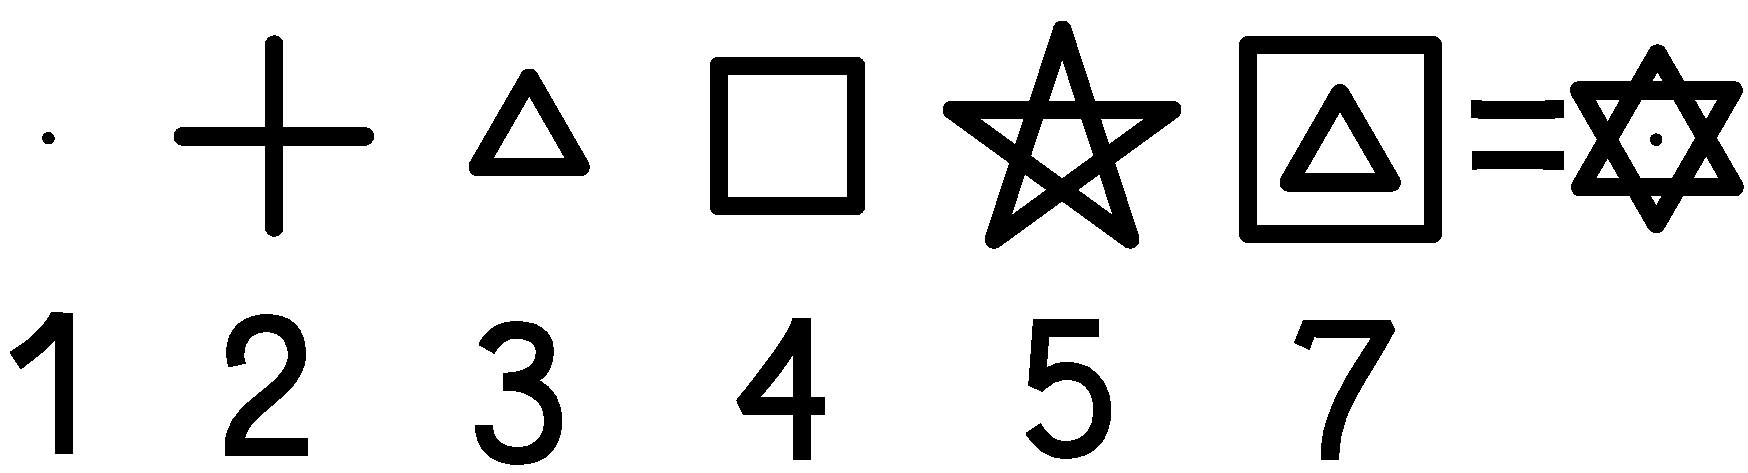
\includegraphics[width=0.3\columnwidth]{Concepts/Archetypes}
\end{figure}

\section{Astrology and astronomy}

\subsection{Zodiac signs}

Western zodiac signs originate from the Babylonians (``Chaldea'' in Greek terms, in today's form \(\approx\) \num{400} BC) and also have hellenistic influences. The constellations are located near the solar ekliptic (from Gr. \foreignlanguage{greek}{ἐκλειπτική τροχιά} ekleiptikē trochiá), the path that the sun apparently moves on during the year. Each of the signs occupies \ang{30} of celestial longitude, due to the earth's orbital eccentricity corresponding to \SI{20.4}{d} for Capricorn to \SI{31.4}{d} for cancer.

 \tablehead{
       \toprule
       Character    & Name       &   Description \\
       \midrule }
 \tabletail{\midrule \multicolumn{3}{r}{continued on next page} \\}
 \tablelasttail{\bottomrule}
 \begin{supertabular}{p{0.3\textwidth}p{0.34\textwidth}p{0.34\textwidth}}
  
\includegraphics[width=5mm]{Astrology/Aries}  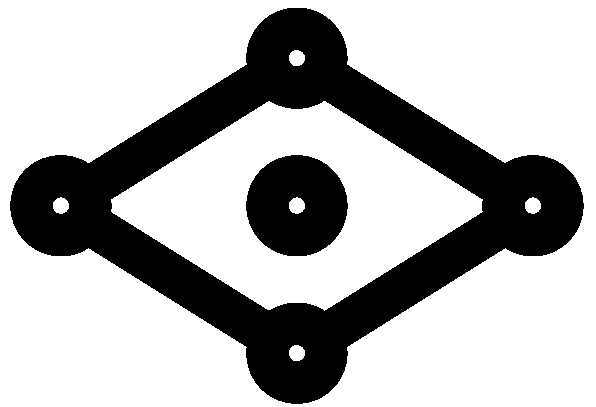
\includegraphics[width=5mm]{Astrology/Aries2} 
\includegraphics[width=5mm]{Astrology/Aries3} 
\includegraphics[width=5mm]{Astrology/Aries4} 
\includegraphics[width=5mm]{Astrology/Aries5} 
\includegraphics[width=5mm]{Astrology/Aries6} 
\includegraphics[width=5mm]{Astrology/Aries7} 
\includegraphics[width=5mm]{Astrology/Aries8} & Aries (Ram) & from the first day of spring (vernal equinox) 21.03. to 20.04. \\
  
\includegraphics[width=5mm]{Astrology/Taurus}   
\includegraphics[width=5mm]{Astrology/Taurus2}  
\includegraphics[width=5mm]{Astrology/Taurus3} 
\includegraphics[width=5mm]{Astrology/Taurus4}  
\includegraphics[width=5mm]{Astrology/Taurus5}  
\includegraphics[width=5mm]{Astrology/Taurus6} 
\includegraphics[width=5mm]{Astrology/Taurus7}  
\includegraphics[width=5mm]{Astrology/Taurus8}  
\includegraphics[width=5mm]{Astrology/Taurus9} 
\includegraphics[width=5mm]{Astrology/Taurus10} 
\includegraphics[width=5mm]{Astrology/Taurus11} 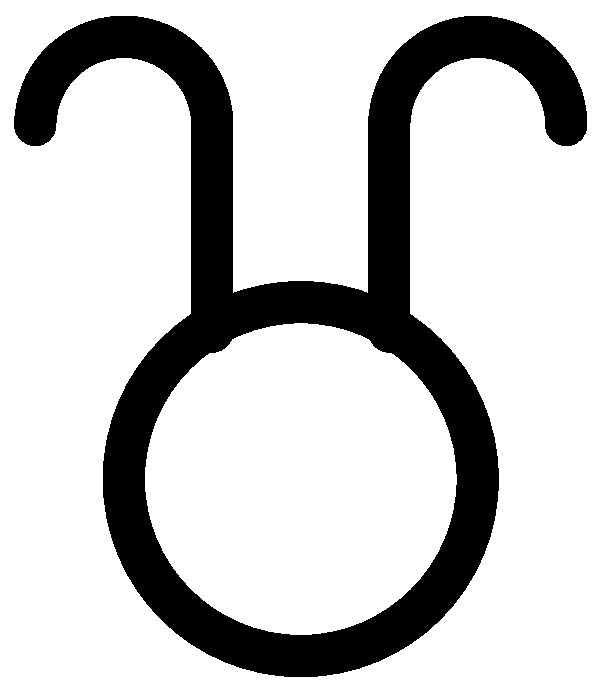
\includegraphics[width=5mm]{Astrology/Taurus12} 
\includegraphics[width=5mm]{Astrology/Taurus13} 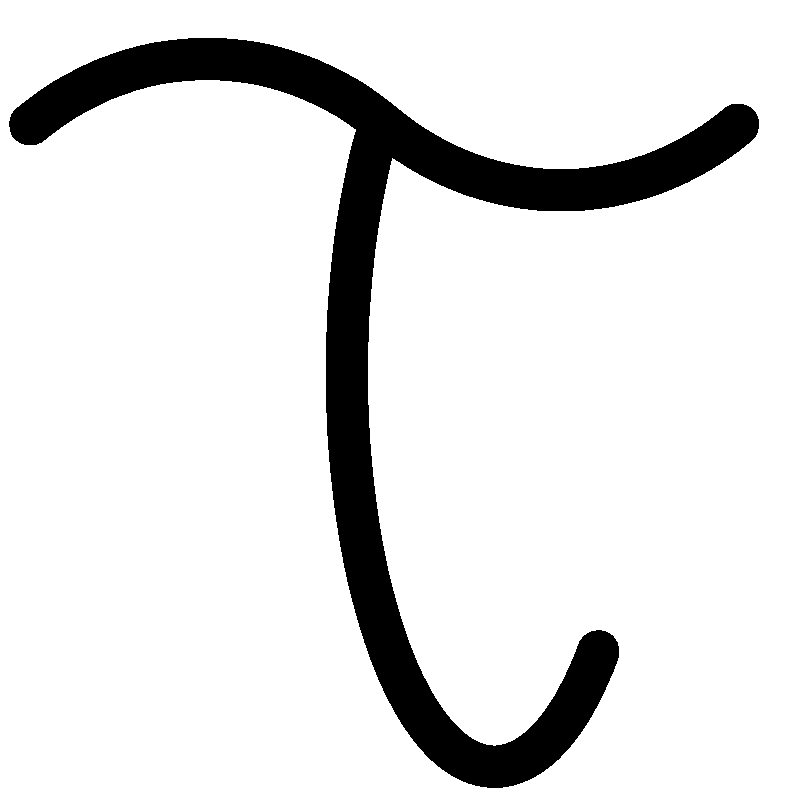
\includegraphics[width=5mm]{Astrology/Taurus14} 
\includegraphics[width=5mm]{Astrology/Taurus15} 
\includegraphics[width=5mm]{Astrology/Taurus16} 
\includegraphics[width=5mm]{Astrology/Taurus17} & Taurus      & 20.04. -- 21.05. \\
  
\includegraphics[width=5mm]{Astrology/Gemini}   
\includegraphics[width=5mm]{Astrology/Gemini2}  
\includegraphics[width=5mm]{Astrology/Gemini3} 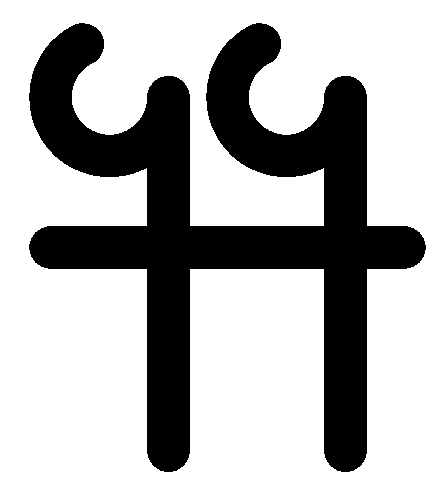
\includegraphics[width=5mm]{Astrology/Gemini4}  
\includegraphics[width=5mm]{Astrology/Gemini5}  
\includegraphics[width=5mm]{Astrology/Gemini6} 
\includegraphics[width=5mm]{Astrology/Gemini7}  
\includegraphics[width=5mm]{Astrology/Gemini8}  
\includegraphics[width=5mm]{Astrology/Gemini9} 
\includegraphics[width=5mm]{Astrology/Gemini10} 
\includegraphics[width=5mm]{Astrology/Gemini11} 
\includegraphics[width=5mm]{Astrology/Gemini12} 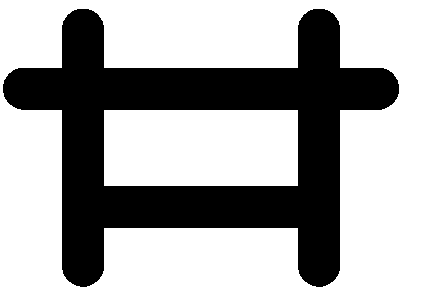
\includegraphics[width=5mm]{Astrology/Gemini13} 
\includegraphics[width=5mm]{Astrology/Gemini14} 
\includegraphics[width=5mm]{Astrology/Gemini15} 
\includegraphics[width=5mm]{Astrology/Gemini16} 
\includegraphics[width=5mm]{Astrology/Gemini17} 
\includegraphics[width=5mm]{Astrology/Gemini19} 
\includegraphics[width=5mm]{Astrology/Gemini20} 
\includegraphics[width=5mm]{Astrology/Gemini21} 
\includegraphics[width=5mm]{Astrology/Gemini22} 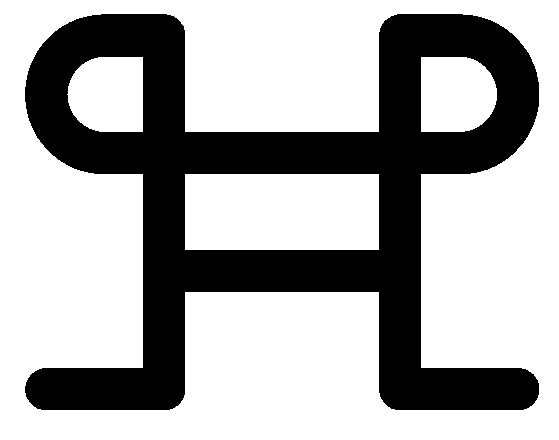
\includegraphics[width=5mm]{Astrology/Gemini23} 
\includegraphics[width=5mm]{Astrology/Gemini24} 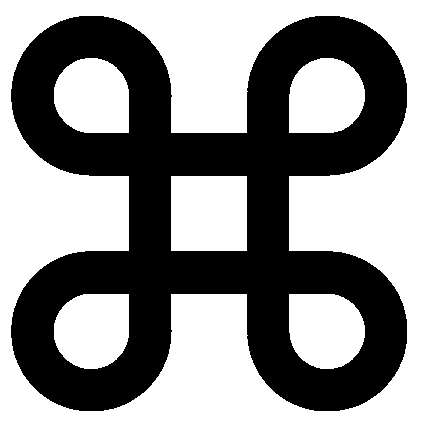
\includegraphics[width=5mm]{Astrology/Gemini25} \includegraphics[width=5mm]{Astrology/Gemini26} \includegraphics[width=5mm]{Astrology/Gemini27}      & Gemini      & 21.05. -- 21.06. \\
  \includegraphics[width=5mm]{Astrology/Cancer}   \includegraphics[width=5mm]{Astrology/Cancer2}  \includegraphics[width=5mm]{Astrology/Cancer3} \includegraphics[width=5mm]{Astrology/Cancer4}  \includegraphics[width=5mm]{Astrology/Cancer5}  \includegraphics[width=5mm]{Astrology/Cancer6} \includegraphics[width=5mm]{Astrology/Cancer7}  \includegraphics[width=5mm]{Astrology/Cancer8}  \includegraphics[width=5mm]{Astrology/Cancer9} \includegraphics[width=5mm]{Astrology/Cancer10} \includegraphics[width=5mm]{Astrology/Cancer11} \includegraphics[width=5mm]{Astrology/Cancer12} \includegraphics[width=5mm]{Astrology/Cancer14}    & Cancer      & 21.06. -- 23.07. \\
  \includegraphics[width=5mm]{Astrology/Leo}   \includegraphics[width=5mm]{Astrology/Leo2}  \includegraphics[width=5mm]{Astrology/Leo3} \includegraphics[width=5mm]{Astrology/Leo4}  \includegraphics[width=5mm]{Astrology/Leo6}  \includegraphics[width=5mm]{Astrology/Leo7} \includegraphics[width=5mm]{Astrology/Leo8}  \includegraphics[width=5mm]{Astrology/Leo9}  \includegraphics[width=5mm]{Astrology/Leo10} \includegraphics[width=5mm]{Astrology/Leo11} \includegraphics[width=5mm]{Astrology/Leo12} \includegraphics[width=5mm]{Astrology/Leo13} \includegraphics[width=5mm]{Astrology/Leo14} \includegraphics[width=5mm]{Astrology/Leo15} \includegraphics[width=5mm]{Astrology/Leo16} \includegraphics[width=5mm]{Astrology/Leo17} \includegraphics[width=5mm]{Astrology/Leo18} \includegraphics[width=5mm]{Astrology/Leo19} \includegraphics[width=5mm]{Astrology/Leo20} \includegraphics[width=5mm]{Astrology/Leo21} \includegraphics[width=5mm]{Astrology/Leo22} & Leo         & 23.07. -- 23.08. \\
  \includegraphics[width=5mm]{Astrology/Virgo}       & Virgo       & 23.08. -- 23.09. \\
  \includegraphics[width=5mm]{Astrology/Libra}   \includegraphics[width=5mm]{Astrology/Libra2}  \includegraphics[width=5mm]{Astrology/Libra3} \includegraphics[width=5mm]{Astrology/Libra4}  \includegraphics[width=5mm]{Astrology/Libra5}  \includegraphics[width=5mm]{Astrology/Libra6} \includegraphics[width=5mm]{Astrology/Libra7}  \includegraphics[width=5mm]{Astrology/Libra8}  \includegraphics[width=5mm]{Astrology/Libra9} \includegraphics[width=5mm]{Astrology/Libra10} \includegraphics[width=5mm]{Astrology/Libra11} & Libra       & 23.09. -- 23.10. \\
  \includegraphics[width=5mm]{Astrology/Scorpio}   \includegraphics[width=5mm]{Astrology/Scorpio2}  \includegraphics[width=5mm]{Astrology/Scorpio3} \includegraphics[width=5mm]{Astrology/Scorpio4}  \includegraphics[width=5mm]{Astrology/Scorpio5}  \includegraphics[width=5mm]{Astrology/Scorpio6} \includegraphics[width=5mm]{Astrology/Scorpio7}  \includegraphics[width=5mm]{Astrology/Scorpio8}  \includegraphics[width=5mm]{Astrology/Scorpio9} \includegraphics[width=5mm]{Astrology/Scorpio10} \includegraphics[width=5mm]{Astrology/Scorpio11} \includegraphics[width=5mm]{Astrology/Scorpio12} \includegraphics[width=5mm]{Astrology/Scorpio13} \includegraphics[width=5mm]{Astrology/Scorpio14} \includegraphics[width=5mm]{Astrology/Scorpio15} \includegraphics[width=5mm]{Astrology/Scorpio16} \includegraphics[width=5mm]{Astrology/Scorpio17} \includegraphics[width=5mm]{Astrology/Scorpio18} \includegraphics[width=5mm]{Astrology/Scorpio19} \includegraphics[width=5mm]{Astrology/Scorpio20} \includegraphics[width=5mm]{Astrology/Scorpio21} \includegraphics[width=5mm]{Astrology/Scorpio22} \includegraphics[width=5mm]{Astrology/Scorpio23} \includegraphics[width=5mm]{Astrology/Scorpio24} \includegraphics[width=5mm]{Astrology/Scorpio25} & Scorpio     & 23.10. -- 22.11. \\
  \includegraphics[width=5mm]{Astrology/Sagittarius}   \includegraphics[width=5mm]{Astrology/Sagittarius2}  \includegraphics[width=5mm]{Astrology/Sagittarius3} \includegraphics[width=5mm]{Astrology/Sagittarius4}  \includegraphics[width=5mm]{Astrology/Sagittarius5}  \includegraphics[width=5mm]{Astrology/Sagittarius6} \includegraphics[width=5mm]{Astrology/Sagittarius7}  \includegraphics[width=5mm]{Astrology/Sagittarius8}  \includegraphics[width=5mm]{Astrology/Sagittarius9} \includegraphics[width=5mm]{Astrology/Sagittarius10} \includegraphics[width=5mm]{Astrology/Sagittarius11} \includegraphics[width=5mm]{Astrology/Sagittarius12} \includegraphics[width=5mm]{Astrology/Sagittarius13} \includegraphics[width=5mm]{Astrology/Sagittarius14} \includegraphics[width=5mm]{Astrology/Sagittarius15} \includegraphics[width=5mm]{Astrology/Sagittarius16} \includegraphics[width=5mm]{Astrology/Sagittarius17} \includegraphics[width=5mm]{Astrology/Sagittarius18} \includegraphics[width=5mm]{Astrology/Sagittarius19} \includegraphics[width=5mm]{Astrology/Sagittarius20} \includegraphics[width=5mm]{Astrology/Sagittarius21} \includegraphics[width=5mm]{Astrology/Sagittarius22} \includegraphics[width=5mm]{Astrology/Sagittarius23} \includegraphics[width=5mm]{Astrology/Sagittarius24} \includegraphics[width=5mm]{Astrology/Sagittarius25} \includegraphics[width=5mm]{Astrology/Sagittarius26} \includegraphics[width=5mm]{Astrology/Sagittarius27} & Sagittarius & 23.11. -- 22.12. \\
  \includegraphics[width=5mm]{Astrology/Capricorn}   \includegraphics[width=5mm]{Astrology/Capricorn2}  \includegraphics[width=5mm]{Astrology/Capricorn3} \includegraphics[width=5mm]{Astrology/Capricorn4}  \includegraphics[width=5mm]{Astrology/Capricorn5}  \includegraphics[width=5mm]{Astrology/Capricorn6} \includegraphics[width=5mm]{Astrology/Capricorn7}  \includegraphics[width=5mm]{Astrology/Capricorn8}  \includegraphics[width=5mm]{Astrology/Capricorn9} \includegraphics[width=5mm]{Astrology/Capricorn10} \includegraphics[width=5mm]{Astrology/Capricorn11} \includegraphics[width=5mm]{Astrology/Capricorn12} \includegraphics[width=5mm]{Astrology/Capricorn13} \includegraphics[width=5mm]{Astrology/Capricorn14} \includegraphics[width=5mm]{Astrology/Capricorn15} \includegraphics[width=5mm]{Astrology/Capricorn16} \includegraphics[width=5mm]{Astrology/Capricorn17} \includegraphics[width=5mm]{Astrology/Capricorn18} \includegraphics[width=5mm]{Astrology/Capricorn19} \includegraphics[width=5mm]{Astrology/Capricorn20} \includegraphics[width=5mm]{Astrology/Capricorn21} \includegraphics[width=5mm]{Astrology/Capricorn22} \includegraphics[width=5mm]{Astrology/Capricorn23} \includegraphics[width=5mm]{Astrology/Capricorn24} \includegraphics[width=5mm]{Astrology/Capricorn25} \includegraphics[width=5mm]{Astrology/Capricorn26} \includegraphics[width=5mm]{Astrology/Capricorn27} \includegraphics[width=5mm]{Astrology/Capricorn28} \includegraphics[width=5mm]{Astrology/Capricorn29} \includegraphics[width=5mm]{Astrology/Capricorn30} \includegraphics[width=5mm]{Astrology/Capricorn31} & Capricorn   & 22.12. -- 20.01. \\
  \includegraphics[width=5mm]{Astrology/Aquarius} \includegraphics[width=5mm]{Astrology/Aquarius2} \includegraphics[width=5mm]{Astrology/Aquarius3} \includegraphics[width=5mm]{Astrology/Aquarius4} & Aquarius    & 20.01. -- 19.02. \\
  \includegraphics[width=5mm]{Astrology/Pisces}   \includegraphics[width=5mm]{Astrology/Pisces2}  \includegraphics[width=5mm]{Astrology/Pisces3} \includegraphics[width=5mm]{Astrology/Pisces4}  \includegraphics[width=5mm]{Astrology/Pisces5}  \includegraphics[width=5mm]{Astrology/Pisces6} \includegraphics[width=5mm]{Astrology/Pisces7}  \includegraphics[width=5mm]{Astrology/Pisces8}  \includegraphics[width=5mm]{Astrology/Pisces9} \includegraphics[width=5mm]{Astrology/Pisces10} \includegraphics[width=5mm]{Astrology/Pisces11} \includegraphics[width=5mm]{Astrology/Pisces12} \includegraphics[width=5mm]{Astrology/Pisces13} \includegraphics[width=5mm]{Astrology/Pisces14} \includegraphics[width=5mm]{Astrology/Pisces15} \includegraphics[width=5mm]{Astrology/Pisces16} \includegraphics[width=5mm]{Astrology/Pisces17} \includegraphics[width=5mm]{Astrology/Pisces18} & Pisces      & 19.02. -- 21.03. \\
  \midrule
  \includegraphics[width=5mm]{Astrology/Ophiuchus}   & Ophiuchus   & Serpent-bearer, 30.11. -- 17.12. \\
  \includegraphics[width=5mm]{Astrology/Orion}       & Orion       & \\
  \end{supertabular}

\subsection{Solar system}

\subsubsection{Planets}

Since planets correspond to metals (Mercury -- Mercury, Venus -- Copper, Mars -- Iron \Foreign{etc.}), the symbols for the planet may be used for the metal and \Foreign{vice versa}.


 \tablehead{
       \toprule
       Character    & Name       &   Description \\
       \midrule }
 \tabletail{\midrule \multicolumn{3}{r}{continued on next page} \\}
 \tablelasttail{\bottomrule} \label{tab:solar}
 \begin{supertabular}{p{0.3\textwidth}p{0.34\textwidth}p{0.34\textwidth}}
  \includegraphics[width=5mm]{Astrology/Mercury} & Mercury & \\
  \includegraphics[width=5mm]{Astrology/Venus}   & Venus   & \\
  \includegraphics[width=5mm]{Astrology/Earth} \includegraphics[width=5mm]{Astrology/Earth2}  & Earth   & \\
  \includegraphics[width=5mm]{Astrology/Mars}   \includegraphics[width=5mm]{Astrology/Mars2}  \includegraphics[width=5mm]{Astrology/Mars3} \includegraphics[width=5mm]{Astrology/Mars4}  \includegraphics[width=5mm]{Astrology/Mars5}  \includegraphics[width=5mm]{Astrology/Mars6} \includegraphics[width=5mm]{Astrology/Mars7}  \includegraphics[width=5mm]{Astrology/Mars8}  \includegraphics[width=5mm]{Astrology/Mars9} \includegraphics[width=5mm]{Astrology/Mars10} \includegraphics[width=5mm]{Astrology/Mars11} \includegraphics[width=5mm]{Astrology/Mars12} \includegraphics[width=5mm]{Astrology/Mars13} \includegraphics[width=5mm]{Astrology/Mars14} \includegraphics[width=5mm]{Astrology/Mars15} \includegraphics[width=5mm]{Astrology/Mars16} \includegraphics[width=5mm]{Astrology/Mars17} \includegraphics[height=5mm]{Astrology/Mars18} \includegraphics[width=5mm]{Astrology/Mars19} \includegraphics[width=5mm]{Astrology/Mars20} \includegraphics[width=5mm]{Astrology/Mars21} \includegraphics[width=5mm]{Astrology/Mars22} \includegraphics[width=5mm]{Astrology/Mars23} & Mars    & \\
  \includegraphics[width=5mm]{Astrology/Jupiter}   \includegraphics[width=5mm]{Astrology/Jupiter2}  \includegraphics[width=5mm]{Astrology/Jupiter3} \includegraphics[width=5mm]{Astrology/Jupiter4}  \includegraphics[width=5mm]{Astrology/Jupiter5}  \includegraphics[width=5mm]{Astrology/Jupiter6} \includegraphics[width=5mm]{Astrology/Jupiter7}  \includegraphics[width=5mm]{Astrology/Jupiter8}  \includegraphics[width=5mm]{Astrology/Jupiter9} \includegraphics[width=5mm]{Astrology/Jupiter11} \includegraphics[width=5mm]{Astrology/Jupiter12} \includegraphics[width=5mm]{Astrology/Jupiter13} \includegraphics[width=5mm]{Astrology/Jupiter14} \includegraphics[width=5mm]{Astrology/Jupiter15} \includegraphics[width=5mm]{Astrology/Jupiter16} \includegraphics[width=5mm]{Astrology/Jupiter17} \includegraphics[height=5mm]{Astrology/Jupiter18} \includegraphics[width=5mm]{Astrology/Jupiter19} \includegraphics[width=5mm]{Astrology/Jupiter20} \includegraphics[width=5mm]{Astrology/Jupiter21} \includegraphics[width=5mm]{Astrology/Jupiter22} \includegraphics[width=5mm]{Astrology/Jupiter23} \includegraphics[width=5mm]{Astrology/Jupiter24} \includegraphics[width=5mm]{Astrology/Jupiter25} \includegraphics[width=5mm]{Astrology/Jupiter26} \includegraphics[width=5mm]{Astrology/Jupiter27} \includegraphics[width=5mm]{Astrology/Jupiter28} \includegraphics[width=5mm]{Astrology/Jupiter29} \includegraphics[width=5mm]{Astrology/Jupiter30} \includegraphics[width=5mm]{Astrology/Jupiter31} \includegraphics[width=5mm]{Astrology/Jupiter32} \includegraphics[width=5mm]{Astrology/Jupiter33} \includegraphics[width=5mm]{Astrology/Jupiter34} \includegraphics[width=5mm]{Astrology/Jupiter35} \includegraphics[width=5mm]{Astrology/Jupiter36} & Jupiter & \\
  \includegraphics[width=5mm]{Astrology/Saturn}   \includegraphics[width=5mm]{Astrology/Saturn2}  \includegraphics[width=5mm]{Astrology/Saturn3} \includegraphics[width=5mm]{Astrology/Saturn4}  \includegraphics[width=5mm]{Astrology/Saturn5}  \includegraphics[width=5mm]{Astrology/Saturn6} \includegraphics[width=5mm]{Astrology/Saturn7}  \includegraphics[width=5mm]{Astrology/Saturn8}  \includegraphics[width=5mm]{Astrology/Saturn9} \includegraphics[width=5mm]{Astrology/Saturn10} \includegraphics[width=5mm]{Astrology/Saturn11} \includegraphics[width=5mm]{Astrology/Saturn12} \includegraphics[width=5mm]{Astrology/Saturn13} \includegraphics[width=5mm]{Astrology/Saturn14} \includegraphics[width=5mm]{Astrology/Saturn15} \includegraphics[width=5mm]{Astrology/Saturn16} \includegraphics[width=5mm]{Astrology/Saturn17} \includegraphics[width=5mm]{Astrology/Saturn18} \includegraphics[width=5mm]{Astrology/Saturn19} \includegraphics[width=5mm]{Astrology/Saturn20} \includegraphics[width=5mm]{Astrology/Saturn21} \includegraphics[width=5mm]{Astrology/Saturn22} \includegraphics[width=5mm]{Astrology/Saturn23} \includegraphics[width=5mm]{Astrology/Saturn24} \includegraphics[width=5mm]{Astrology/Saturn25} \includegraphics[width=5mm]{Astrology/Saturn26} \includegraphics[width=5mm]{Astrology/Saturn27} \includegraphics[width=5mm]{Astrology/Saturn28} \includegraphics[width=5mm]{Astrology/Saturn29} \includegraphics[width=5mm]{Astrology/Saturn30} \includegraphics[width=5mm]{Astrology/Saturn31} \includegraphics[width=5mm]{Astrology/Saturn32} \includegraphics[width=5mm]{Astrology/Saturn33} \includegraphics[width=5mm]{Astrology/Saturn34} \includegraphics[width=5mm]{Astrology/Saturn35} \includegraphics[width=5mm]{Astrology/Saturn36} \includegraphics[width=5mm]{Astrology/Saturn37} \includegraphics[width=5mm]{Astrology/Saturn38} \includegraphics[width=5mm]{Astrology/Saturn39} \includegraphics[width=5mm]{Astrology/Saturn40} \includegraphics[width=5mm]{Astrology/Saturn41} & Saturn  & \\
  \includegraphics[width=5mm]{Astrology/Uranus} \includegraphics[width=5mm]{Astrology/Uranus2}   \includegraphics[width=5mm]{Astrology/Uranus3} \includegraphics[width=5mm]{Astrology/Uranus4}  & Uranus (Herschel) & \\
  \includegraphics[width=5mm]{Astrology/Neptun}  & Neptun  & \\
  \includegraphics[width=5mm]{Astrology/Pluto} \includegraphics[width=5mm]{Astrology/Pluto2}  & Pluto   & \\
  \end{supertabular}

\subsubsection{Asteroids}

 \tablehead{
       \toprule
       Character    & Name       &   Description \\
       \midrule }
 \tabletail{\midrule \multicolumn{3}{r}{continued on next page} \\}
 \tablelasttail{\bottomrule}
 \begin{supertabular}{p{0.3\textwidth}p{0.34\textwidth}p{0.34\textwidth}}
    \includegraphics[width=5mm]{Astrology/Ceres} \includegraphics[width=5mm]{Astrology/Ceres2} \includegraphics[width=5mm]{Astrology/Ceres3} & (1) Ceres         & \\
    \includegraphics[width=5mm]{Astrology/Pallas} \includegraphics[width=5mm]{Astrology/Pallas2} \includegraphics[width=5mm]{Astrology/Pallas3} & (2) Pallas        & \\
    \includegraphics[width=5mm]{Astrology/Juno} \includegraphics[width=5mm]{Astrology/Juno2} \includegraphics[width=5mm]{Astrology/Juno3} & (3) Juno          & \\
    \includegraphics[width=5mm]{Astrology/Vesta}      & (4) Vesta         & \\
    \includegraphics[width=5mm]{Astrology/Astraea}    & (5) Astraea       & \\
    \includegraphics[width=5mm]{Astrology/Hebe}       & (6) Hebe          & \\
    \includegraphics[width=5mm]{Astrology/Apollo} \includegraphics[width=5mm]{Astrology/Apollo2}    & (1862) Apollo     & \\
    \includegraphics[width=5mm]{Astrology/Sysyphus}   & (1866) Sisyphus   & \\
    \includegraphics[width=5mm]{Astrology/Chiron}     & (2060) Chiron     & \\
    \includegraphics[width=5mm]{Astrology/Aten}       & (2062) Aten       & \\
                                                      & (2100) Ra-Shalom  & \\
    \includegraphics[width=5mm]{Astrology/Adonis}     & (2101) Adonis     & \\
    \includegraphics[width=5mm]{Astrology/Hathor}     & (2340) Hathor     & \\
    \includegraphics[width=5mm]{Astrology/Cruinthne}  & (3753) Cruinthne  & \\
    \includegraphics[width=5mm]{Astrology/Toutatis}   & (4179) Toutatis   & \\
    \includegraphics[width=5mm]{Astrology/Hermes}     & (69230) Hermes    & \\
    \includegraphics[width=5mm]{Astrology/Apophis}    & (99942) Apophis   & near-earth passage 2029-04-13 \\
                                                      & (367943) Duende   & near-earth passage 2013-02-15 \\
    \end{supertabular}


\subsubsection{Planetoids of the \Name{Kuiper} belt}

The most well-known object of this class is Pluto, which is officially no longer a planet.

 \tablehead{
       \toprule
       Character    & Name       &   Description \\
       \midrule }
 \tabletail{\midrule \multicolumn{3}{r}{continued on next page} \\}
 \tablelasttail{\bottomrule}
 \begin{supertabular}{p{0.3\textwidth}p{0.34\textwidth}p{0.34\textwidth}}
  \includegraphics[width=5mm]{Astrology/Eris1} \includegraphics[width=5mm]{Astrology/Eris2} & (136199) Eris  & \\
  \includegraphics[width=5mm]{Astrology/Gonggong} & (225088) Gonggong & \\
  \includegraphics[width=5mm]{Astrology/Haumea}   & (136108) Haumea  & \\
  \includegraphics[width=5mm]{Astrology/Makemake} & (136472) Makemake  & \\
  \includegraphics[width=5mm]{Astrology/Orcus} \includegraphics[width=5mm]{Astrology/Orcus2} & (90482) Orcus  & \\
  \includegraphics[width=5mm]{Astrology/Quaoar}   & (50000) Quaoar   & \\
  \includegraphics[width=5mm]{Astrology/Sedna}    & (90377) Sedna  & \\
  \end{supertabular}

\subsection{Important stars}

 \tablehead{
       \toprule
       Character    & Name       &   Description \\
       \midrule }
 \tabletail{\midrule \multicolumn{3}{r}{continued on next page} \\}
 \tablelasttail{\bottomrule}
 \begin{supertabular}{p{0.3\textwidth}p{0.34\textwidth}p{0.34\textwidth}}
  \includegraphics[width=5mm]{Astrology/Aldebaran}        & Aldebaran  &  \\
  \includegraphics[width=7mm]{Astrology/Alphecca} \includegraphics[width=7mm]{Astrology/Alphecca2} & \Foreign{alpha coronae borealis},  Alphecca  &  \\
  \includegraphics[width=5mm]{Astrology/Amalthea} \includegraphics[width=5mm]{Astrology/Capella} & \Foreign{Alpha aurigae}, Amalthea, Hircus, Capella, Alayoch   &  \\
  \includegraphics[width=5mm]{Astrology/Arcturus} \includegraphics[width=5mm]{Astrology/Arcturus2} & \Foreign{alpha Bootis}, Arcturus, Alchameth  &  \\
  \includegraphics[width=5mm]{Astrology/betaPersei} \includegraphics[width=5mm]{Astrology/betaPersei2} \includegraphics[width=5mm]{Astrology/betaPersei3} & \Foreign{\textbeta\ Persei, caput algol} & \\
  \includegraphics[width=5mm]{Astrology/CanisMajor} \includegraphics[width=5mm]{Astrology/CanisMajor2} & \Foreign{Canis major}, Sirius & \\
  \includegraphics[width=5mm]{Astrology/CanisMinor} & \Foreign{Canis minor}, Procyon & \\
  \includegraphics[width=5mm]{Astrology/CaudaCapricorni} & \Foreign{Cauda Capricorni, \textdelta\ Capricorni, Deneb Algedi} & \\
  \includegraphics[width=5mm]{Astrology/CaudaLeonis} \includegraphics[width=5mm]{Astrology/CaudaLeonis2} \includegraphics[width=5mm]{Astrology/CaudaLeonis3} \includegraphics[width=5mm]{Astrology/CaudaLeonis4} & \Foreign{Cauda leonis, finis Leonis et principis Virginia, \textbeta\ leonis}, \foreignlanguage{arabic}{ذنب الاسد} \Foreign{ðanab al-asad} (lion's tail),  Denebola & \\
  \includegraphics[width=5mm]{Astrology/CaudaScorpionis} \includegraphics[width=5mm]{Astrology/CaudaScorpionis2} \includegraphics[width=5mm]{Astrology/CaudaScorpionis3} \includegraphics[width=5mm]{Astrology/CaudaScorpionis4} & \Foreign{Cauda scorpionis, finis Scorpionis et caput Sagittarii, \textlambda\ Scorpii}, \foreignlanguage{arabic}{الشولاء} \Foreign{al-šawlā}, Shaula & \\
  \includegraphics[width=5mm]{Astrology/CaudaUrsae} \includegraphics[width=5mm]{Astrology/CaudaUrsae2} \includegraphics[width=5mm]{Astrology/CaudaUrsae3} & \Foreign{\textalpha\ Ursae Minoris, Stella Polaris, Cynosura} & Pole star \\
  \includegraphics[width=5mm]{Astrology/CorLeonis} \includegraphics[width=5mm]{Astrology/CorLeonis2} \includegraphics[width=5mm]{Astrology/CorLeonis3} & \Foreign{Cor Leonis, \textalpha\ Leonis}, ‘the little king’ & \\
  \includegraphics[width=5mm]{Astrology/CorScorpionis} \includegraphics[width=5mm]{Astrology/CorScorpionis2} \includegraphics[width=5mm]{Astrology/CorScorpionis3} & \Foreign{Cor Scorpionis, \textalpha\ Scorpii}, Antares  & \\
  \includegraphics[width=5mm]{Astrology/Regulus1} \includegraphics[width=5mm]{Astrology/Regulus2} \includegraphics[width=5mm]{Astrology/Regulus3} \includegraphics[width=5mm]{Astrology/Regulus4}         & Regulus             & brightest star system (apparent magnitude of +1.35) in the constellation Leo (\textalpha\ Leonis). \\
  \includegraphics[width=7mm]{Astrology/DeltaCorvus}      & \Foreign{\textdelta\ corvi, Ala corvi}, Algorab  & double star \\
  \includegraphics[width=7mm]{Astrology/Pleiades} \includegraphics[width=7mm]{Astrology/Pleiades2} \includegraphics[width=7mm]{Astrology/Pleiades3} & Pleiades & \\
  \includegraphics[width=7mm]{Astrology/Spica} & Spica (\textalpha\ \Foreign{virginis}) & \\
 \end{supertabular}

\subsection{Other}

\begin{figure}
 \caption{\capstart Ptolemaic aspects. For details see text. }
 \label{fig:Aspect}
 \centering
 \includegraphics[width=0.5\textwidth]{Astrology/Aspect}
\end{figure}

According to  \parencite{Pto-00}, the angle between two objects as seen by an observer on earth are described by the following terms (see also fig. \ref{fig:Aspect}):

\begin{description}
   \item[Conjunction]{\includegraphics[width=5mm]{Astrology/Conjunction} \includegraphics[width=5mm]{Astrology/Conjunction2} angle of \(\frac{0}{12} \ang{360} = \ang{0}\). Objects appear close together on the celestial sphere (within \(\pm \ang{10}\)). The minimal distance is called \emph{appulse}. With respect to the sun, an object -- as seen from earth -- can be in
      \begin{description}
        \item[superior conjunction]{it appears to be behind the sun }
        \item[inferior conjunction]{it appears to be in front of the sun}
      \end{description}
      At new moon, the moon is in inferior conjunction with the sun.
      There are special sigils for planetary conjunctions:
      \begin{description}
        \item[Jupiter and Saturn]{\includegraphics[width=5mm]{Astrology/ConjunctionJupiterSaturn} \includegraphics[width=5mm]{Astrology/ConjunctionJupiterSaturn2} \includegraphics[width=5mm]{Astrology/ConjunctionJupiterSaturn3} is called \emph{great conjunction}, the one in 7 BC may be the \emph{Star of Bethlehem} (Mt. 2\textsubscript{2}).}
        \item[Saturn and Mars]{\includegraphics[width=5mm]{Astrology/ConjunctionSaturnMars} \includegraphics[width=5mm]{Astrology/ConjunctionSaturnMars2} }
        \item[Jupiter, Saturn and Mars]{\includegraphics[width=5mm]{Astrology/ConjunctionJupiterSaturnMars} \includegraphics[width=5mm]{Astrology/ConjunctionJupiterSaturnMars2} }
      \end{description} }
   \item[Semisextile]{\includegraphics[width=5mm]{Astrology/Semisextile} \includegraphics[width=5mm]{Astrology/Semisextile2} \includegraphics[width=5mm]{Astrology/Semisextile3} \includegraphics[width=5mm]{Astrology/Semisextile4} angle of \(\frac{1}{12} \ang{360} = \ang{30}\) }
   \item[Sextile]{\includegraphics[width=5mm]{Astrology/Sextile} angle of \(\frac{2}{12} \ang{360} = \ang{60}\) }
   \item[Semisquare]{\includegraphics[width=5mm]{Astrology/SemiSquare} \includegraphics[width=5mm]{Astrology/SemiSquare2} angle of \(1/2 \frac{3}{12} \ang{360} = \ang{45}\), \Foreign{tetragonum} }
   \item[Square]{\includegraphics[width=5mm]{Astrology/Square} \includegraphics[width=5mm]{Astrology/Square2} angle of \(\frac{3}{12} \ang{360} = \ang{90}\) }
   \item[Trine]{\includegraphics[width=5mm]{Astrology/Trine} angle of \(\frac{4}{12} \ang{360} = \ang{120}\) }
   \item[Quincunx]{\includegraphics[width=5mm]{Astrology/Quincunx} \includegraphics[width=5mm]{Astrology/Quincunx2} \includegraphics[width=5mm]{Astrology/Quincunx3} \includegraphics[width=5mm]{Astrology/Quincunx4} angle of \(\frac{5}{12} \ang{360} = \ang{150}\) }
   \item[Opposition]{\includegraphics[width=5mm]{Astrology/Opposition} angle of \(\frac{6}{12} \ang{360} = \ang{180}\) earth is exactly between the objects.}
   \item[Eclipse]{one object moves into the shadow of another during an opposition (\Foreign{e.g.}, the moon into the shadow of the earth during a lunar eclipse). }
   \item[Transit]{an apparently smaller object moves in front of a larger during conjunction. For example, Venus or Mercury may pass in front of the sun as black spots. }
   \item[Occultation]{\includegraphics[width=5mm]{Astrology/Occultation} during conjunction, an apparently larger object moves in front of a smaller and hides it. For example, in a solar eclipse the moon passes between earth and sun, hiding it. The moon is much smaller than the sun, but also much closer to earth, so that both appear to have about the same diameter. Occultation of planets by the moon also occur relatively frequently.}
 \end{description}

Aspects introduced by other authors include
\begin{description}
   \item[Decile, ]{angle of \(\frac{1}{10} \ang{360} = \ang{36}\) \includegraphics[width=5mm]{Astrology/Decile}}
   \item[Octile]{angle of \(\frac{1}{8} \ang{360} = \ang{45}\) \includegraphics[width=5mm]{Astrology/Octile}}
   \item[Septile]{angle of \(\frac{1}{7} \ang{360} = \ang{45;25;0}\) \includegraphics[width=5mm]{Astrology/Septile} \includegraphics[width=5mm]{Astrology/Septile2}}
   \item[Quintile]{angle of \(\frac{1}{5} \ang{360} = \ang{72}\) \includegraphics[width=5mm]{Astrology/Quintile}}
   \item[Bisquintile, sesquiquintile]{angle of \(\frac{3}{10} \ang{360} = \ang{72} + \ang{36} = \ang{108}\) \includegraphics[width=5mm]{Astrology/Bisquintile} \includegraphics[width=5mm]{Astrology/Bisquintile2} \includegraphics[width=5mm]{Astrology/Bisquintile3}}
   \item[Trioctile, sesquiquadrate]{angle of \(\frac{3}{8} \ang{360} = \ang{90} + \ang{45} = \ang{135}\) \includegraphics[width=5mm]{Astrology/Trioctile} \includegraphics[width=5mm]{Astrology/Trioctile2} \includegraphics[width=5mm]{Astrology/Trioctile3} \includegraphics[width=5mm]{Astrology/Trioctile4} }
   \item[Bisquintile]{angle of \(\frac{2}{5} \ang{360} = \ang{144}\) \includegraphics[width=5mm]{Astrology/Bisquintile} \includegraphics[width=5mm]{Astrology/Bisquintile2}}
\end{description}


A horoskop (from Gr. \foreignlanguage{greek}{ὥρα σκοπεῖν} hōra skopéin = marker of the hour [of birth]) or natal chart was based on the theory that the movement of heavenly objects was causally linked to the events on earth (``like above, so below''). For this purpose were determined the
\begin{itemize}
  \item{\Foreign{prima domus} (first house, ascendant), intersection of ekliptic and horizon, east angle}
  \item{\Foreign{medium coeli} (midheaven, 10th house), intersection of meridian and ekliptic, north angle}
  \item{Descendant, setting sign, west angle }
  \item{\Foreign{imum coeli} (opposite of \Foreign{medium coeli}), south angle}
\end{itemize}
as function of time and place of birth, using the geocentric perspective. Together, these form a cross.

If the plane defined by the orbit of a celestial body has an angle (inclination) \(\neq 0\) to a reference plane, then the orbit intersects the reference plane in two points. The one crossed by the north-moving body is called the ascending node (Latin \Foreign{caput draconis} = dragon's head or Greek \foreignlanguage{greek}{αναβιβάζων} anabibazōn). The node of the south-moving body is called descending node (\Foreign{cauda draconis} = dragon's tail or \foreignlanguage{greek}{καταβιβάζων} katabibazōn). In astrology, these terms refer to the crossings of the orbit of the moon with the apparent orbit of the sun across the sky.

The orbit of a celestial body around another is an ellipse and as such has two focal points. One is occupied by the heavier (resting) body, the second is called the \emph{lilith}. It is empty and of no significance in astronomy. In astrology, however, the second focal point of the moon's orbit around earth is called \emph{black moon lilith}.

In extensive scientific studies, if proper blinding is used, there is no significant (beyond what is expected randomly) connection between a horoskop and the character or biography of a person \parencite{Car-83, Fic-83, Wun-08}. In particular, statements about personality are so vague and general that most people will believe they were tailored to them \parencite{For-49} (\Name{Barnum}-effect, named after showman \Name{Phineas Taylor Barnum}, 1810--1891).

 \tablehead{
       \toprule
       Character    & Name       &   Description \\
       \midrule }
 \tabletail{\midrule \multicolumn{3}{r}{continued on next page} \\}
 \tablelasttail{\bottomrule}
 \begin{supertabular}{p{0.3\textwidth}p{0.34\textwidth}p{0.34\textwidth}}
  \includegraphics[width=5mm]{Astrology/Ascendant}  \includegraphics[width=5mm]{Astrology/Ascendant2} \includegraphics[width=5mm]{Astrology/Ascendant3} \includegraphics[width=5mm]{Astrology/Ascendant4} \includegraphics[width=5mm]{Astrology/Ascendant5} \includegraphics[width=5mm]{Astrology/Ascendant6} & \Foreign{prima domus} = first house, ascendant & the zodiacal sign and degree that is ascending on the eastern horizon at the specific time and location\\
  \includegraphics[width=5mm]{Astrology/AscendingNode}  \includegraphics[width=5mm]{Astrology/AscendingNode2} \includegraphics[width=5mm]{Astrology/AscendingNode3} \includegraphics[width=5mm]{Astrology/AscendingNode4} \includegraphics[width=5mm]{Astrology/AscendingNode5} \includegraphics[width=5mm]{Astrology/AscendingNode6} \includegraphics[width=5mm]{Astrology/AscendingNode7}   & Ascending node      &  \\
  \includegraphics[width=5mm]{Astrology/Descendant} & Descendant, setting sign, west angle of a horoscope & \\
  \includegraphics[width=5mm]{Astrology/DescendingNode}  \includegraphics[width=5mm]{Astrology/DescendingNode2} \includegraphics[width=5mm]{Astrology/DescendingNode3} \includegraphics[width=5mm]{Astrology/DescendingNode4} \includegraphics[width=5mm]{Astrology/DescendingNode5} \includegraphics[width=5mm]{Astrology/DescendingNode6} \includegraphics[width=5mm]{Astrology/DescendingNode7} \includegraphics[width=5mm]{Astrology/DescendingNode8} \includegraphics[width=5mm]{Astrology/DescendingNode9} \includegraphics[width=5mm]{Astrology/DescendingNode10} \includegraphics[width=5mm]{Astrology/DescendingNode11} & Descending Node     &  \\
  \includegraphics[width=5mm]{Astrology/Comet}            & Comet               &  \\
  \includegraphics[width=5mm]{Astrology/FixedStar} \includegraphics[width=5mm]{Astrology/FixedStar2} \includegraphics[width=5mm]{Astrology/FixedStar3} \includegraphics[width=5mm]{Astrology/FixedStar4} \includegraphics[width=5mm]{Astrology/FixedStar5} \includegraphics[width=5mm]{Astrology/FixedStar6} \includegraphics[width=5mm]{Astrology/FixedStar7} & Fixed star & \\
  \includegraphics[width=5mm]{Astrology/Horoscope} \includegraphics[width=5mm]{Astrology/Horoscope2} & Horoskope & \\
  \includegraphics[width=5mm]{Astrology/BlackMoonLilith} \includegraphics[width=5mm]{Astrology/BlackMoonLilith2} \includegraphics[width=5mm]{Astrology/BlackMoonLilith3}  & black moon lilith   & second focal point of eliptical moon orbit around earth \\
  \includegraphics[width=5mm]{Astrology/FirstQuarterMoon} \includegraphics[width=5mm]{Astrology/MoonWaxing} & First quarter moon, waxing moon  &  \\
  \includegraphics[width=5mm]{Astrology/LastQuarterMoon} \includegraphics[width=5mm]{Astrology/MoonWanning} & Last quarter moon, wanning moon  &  \\
  \includegraphics[width=5mm]{Astrology/Moon}   \includegraphics[width=5mm]{Astrology/Moon2}  \includegraphics[width=5mm]{Astrology/Moon3} \includegraphics[width=5mm]{Astrology/Moon4}  \includegraphics[width=5mm]{Astrology/Moon5}  \includegraphics[width=5mm]{Astrology/Moon6} \includegraphics[width=5mm]{Astrology/Moon7}  \includegraphics[width=5mm]{Astrology/Moon8}  \includegraphics[width=5mm]{Astrology/Moon9} \includegraphics[width=5mm]{Astrology/Moon10} \includegraphics[width=5mm]{Astrology/Moon11} \includegraphics[width=5mm]{Astrology/Moon12} \includegraphics[width=5mm]{Astrology/Moon13} \includegraphics[width=5mm]{Astrology/Moon14} \includegraphics[width=5mm]{Astrology/Moon15} \includegraphics[width=5mm]{Astrology/Moon16} \includegraphics[width=5mm]{Astrology/Moon17} \includegraphics[width=5mm]{Astrology/Moon18} \includegraphics[width=5mm]{Astrology/Moon19} \includegraphics[width=5mm]{Astrology/Moon20} \includegraphics[width=5mm]{Astrology/Moon21} \includegraphics[width=5mm]{Astrology/Moon22} \includegraphics[width=5mm]{Astrology/Moon23} \includegraphics[width=5mm]{Astrology/Moon24} & Moon                &  \\
  \includegraphics[width=5mm]{Astrology/FullHook} \includegraphics[width=5mm]{Astrology/FullHook2} \includegraphics[width=5mm]{Astrology/FullHook3} \includegraphics[width=5mm]{Astrology/FullHook4} & Fool hook & last full moon before birth \\
  \includegraphics[width=5mm]{Astrology/Cardinality}      & Cardinality         &  \\
  \includegraphics[width=5mm]{Astrology/CardinalCross}    & Cardinal cross      & four planets with square (\ang{90}) aspect \\
  \includegraphics[width=5mm]{Astrology/LotOfFortune}   \includegraphics[width=5mm]{Astrology/LotOfFortune2} \includegraphics[width=5mm]{Astrology/LotOfFortune3} \includegraphics[width=5mm]{Astrology/LotOfFortune4}  \includegraphics[width=5mm]{Astrology/LotOfFortune5} \includegraphics[width=5mm]{Astrology/LotOfFortune6} \includegraphics[width=5mm]{Astrology/LotOfFortune7}  \includegraphics[width=5mm]{Astrology/LotOfFortune8} \includegraphics[width=5mm]{Astrology/LotOfFortune9} \includegraphics[width=5mm]{Astrology/LotOfFortune10} \includegraphics[width=5mm]{Astrology/LotOfFortune11} & Lot of fortune      & or lucky point (Lat. \Foreign{Pars Fortunae}), hypothetical point occupied by the Moon when the Sun is on the ascendant. If other bodies than the sun are meant, their sign is placed next to the pars sign. \\
  \includegraphics[width=5mm]{Astrology/LunarEcclipse} \includegraphics[width=5mm]{Astrology/EclipseMoon}  & Lunar eclipse      &  \\
  \includegraphics[width=5mm]{Astrology/EclipseSun} & Eclipse of the sun & \\
  \includegraphics[width=5mm]{Astrology/MediumCoeli} \includegraphics[width=5mm]{Astrology/MediumCoeli2} & \Foreign{Medium coeli}, midheaven & culminating degree of ecliptic in a horoscope \\
  \includegraphics[width=5mm]{Astrology/Rising} & rising & \\
  \includegraphics[width=5mm]{Astrology/Setting} & setting & \\
  \includegraphics[width=5mm]{Astrology/Sun}   \includegraphics[width=5mm]{Astrology/Sun2}  \includegraphics[width=5mm]{Astrology/Sun3} \includegraphics[width=5mm]{Astrology/Sun4}  \includegraphics[width=5mm]{Astrology/Sun5}  \includegraphics[width=5mm]{Astrology/Sun6} \includegraphics[width=5mm]{Astrology/Sun7}  \includegraphics[width=5mm]{Astrology/Sun8}  \includegraphics[width=5mm]{Astrology/Sun9} \includegraphics[width=5mm]{Astrology/Sun10} \includegraphics[width=5mm]{Astrology/Sun11} \includegraphics[width=5mm]{Astrology/Sun12} \includegraphics[width=5mm]{Astrology/Sun13} \includegraphics[width=5mm]{Astrology/Sun14} \includegraphics[width=5mm]{Astrology/Sun15} \includegraphics[width=5mm]{Astrology/Sun16} \includegraphics[width=5mm]{Astrology/Sun17} \includegraphics[width=5mm]{Astrology/Sun18} \includegraphics[width=5mm]{Astrology/Sun19} \includegraphics[width=5mm]{Astrology/Sun20} \includegraphics[width=5mm]{Astrology/Sun21} \includegraphics[width=5mm]{Astrology/Sun22} \includegraphics[width=5mm]{Astrology/Sun23} \includegraphics[width=5mm]{Astrology/Sun24} \includegraphics[width=5mm]{Astrology/Sun25} \includegraphics[width=5mm]{Astrology/Sun26} \includegraphics[width=5mm]{Astrology/Sun27} \includegraphics[width=5mm]{Astrology/Sun28} \includegraphics[width=5mm]{Astrology/Sun29} \includegraphics[width=5mm]{Astrology/Sun30} \includegraphics[width=5mm]{Astrology/Sun31} \includegraphics[width=5mm]{Astrology/Sun32} \includegraphics[width=5mm]{Astrology/Sun33} \includegraphics[width=5mm]{Astrology/Sun34} \includegraphics[width=5mm]{Astrology/Sun35} \includegraphics[width=5mm]{Astrology/Sun36} \includegraphics[width=5mm]{Astrology/Sun37} \includegraphics[width=5mm]{Astrology/Sun38} & Sun                 & also gold \\
  \includegraphics[width=5mm]{Astrology/Transpluto} & Transpluto & \\
\end{supertabular}

\section{Compounds}

In general, \emph{crocus of} or \emph{saffron of} means a yellow compound, \emph{magistery of} a compound purified by precipitation, \emph{magistry of} a compound synthesised from the element and hence without impurities. \emph{Flores} or \emph{flower of} means substances purified by sublimation. \emph{Mercury of} refers to philosophical mercury and can mean anything. \emph{Spritus} refers to volatile compounds, \emph{dead} substances are those where the spiritus (life) has been removed by heating. \emph{Hepar} = liver are brownish substances, often containing sulphur. \emph{Calx} = ashes are substances that have been heated until they glowed. A regulus is a metal drop after smelting.

Vitriol are sulphates, often named by their colour: green -- iron, blue -- copper, white -- zinc, red -- cobalt. Also named by their origin: roman -- iron, cyprian -- copper. Hungarian vitriol was originally copper sulphate, but as the copper in the mines was depleted in the 18th century, it contained more and more iron.

 \tablehead{
       \toprule
       Character    & Name       &   Description \\
       \midrule }
 \tabletail{\midrule \multicolumn{3}{r}{continued on next page} \\}
 \tablelasttail{\bottomrule} \label{tab:Compounds}
 \begin{supertabular}{p{0.3\textwidth}p{0.34\textwidth}p{0.34\textwidth}}
   \includegraphics[width=5mm]{Compounds/Acid} \includegraphics[width=5mm]{Compounds/Acid2} & Acid  & \\
   \includegraphics[width=5mm]{Compounds/AesViride} \includegraphics[width=5mm]{Compounds/AesViride2} \includegraphics[width=5mm]{Compounds/AesViride3} \includegraphics[width=5mm]{Compounds/AesViride4} \includegraphics[width=5mm]{Compounds/AesViride5} \includegraphics[width=5mm]{Compounds/AesViride6} \includegraphics[width=5mm]{Compounds/AesViride7} \includegraphics[width=5mm]{Compounds/AesViride8} \includegraphics[width=5mm]{Compounds/AesViride9} \includegraphics[width=5mm]{Compounds/AesViride10} \includegraphics[width=8mm]{Compounds/AesViride11} \includegraphics[width=5mm]{Compounds/AesViride12} & \Foreign{æs viride, flores virides æris, æris crystalli ærugo}, Spanish green, crystallised verdigris, Hoganit   & Copper(II) acetate \\
   \includegraphics[width=5mm]{Compounds/Alumn} \includegraphics[width=5mm]{Compounds/Alumn2} \includegraphics[width=5mm]{Compounds/Alumn3} \includegraphics[width=5mm]{Compounds/Alumn4} \includegraphics[width=5mm]{Compounds/Alumn5} \includegraphics[width=5mm]{Compounds/Alumn6} \includegraphics[width=5mm]{Compounds/Alumn7} \includegraphics[width=5mm]{Compounds/Alumn8} \includegraphics[width=5mm]{Compounds/Alumn10} \includegraphics[width=5mm]{Compounds/Alumn11} \includegraphics[width=5mm]{Compounds/Alumn12} \includegraphics[width=5mm]{Compounds/Alumn13} \includegraphics[width=5mm]{Compounds/Alumn14} \includegraphics[width=5mm]{Compounds/Alumn15} \includegraphics[width=5mm]{Compounds/Alumn16} \includegraphics[width=5mm]{Compounds/Alumn17} \includegraphics[width=5mm]{Compounds/Alumn18} \includegraphics[width=5mm]{Compounds/Alumn19} & \Foreign{Alumen}, Alum  & Double salt of a Metal(I) and a Metal(III) sulphate, usually \chemical{KAl(SO_4)_2 \times 12 H_2O}\\
   \includegraphics[width=5mm]{Compounds/BurnedAlum} \includegraphics[width=5mm]{Compounds/BurnedAlum2} \includegraphics[width=5mm]{Compounds/BurnedAlum3} \includegraphics[width=5mm]{Compounds/BurnedAlum4} \includegraphics[width=5mm]{Compounds/BurnedAlum5} \includegraphics[width=5mm]{Compounds/BurnedAlum6} \includegraphics[width=5mm]{Compounds/BurnedAlum7} \includegraphics[width=5mm]{Compounds/BurnedAlum8} \includegraphics[width=5mm]{Compounds/BurnedAlum9} \includegraphics[width=5mm]{Compounds/BurnedAlum10} \includegraphics[width=5mm]{Compounds/BurnedAlum11} \includegraphics[width=5mm]{Compounds/BurnedAlum12} & \Foreign{Alumen calcinatum, alumen ustum}, burned alum & anhydride of alum \\
   \includegraphics[width=5mm]{Compounds/AlumenPlumeum} \includegraphics[width=5mm]{Compounds/AlumenPlumeum2} \includegraphics[width=5mm]{Compounds/AlumenPlumeum3} \includegraphics[width=5mm]{Compounds/AlumenPlumeum4} \includegraphics[width=5mm]{Compounds/AlumenPlumeum5} \includegraphics[width=5mm]{Compounds/AlumenPlumeum6} \includegraphics[width=5mm]{Compounds/AlumenPlumeum7} \includegraphics[width=5mm]{Compounds/AlumenPlumeum8} \includegraphics[width=5mm]{Compounds/AlumenPlumeum9} \includegraphics[width=5mm]{Compounds/AlumenPlumeum10} \includegraphics[width=5mm]{Compounds/AlumenPlumeum11} \includegraphics[width=5mm]{Compounds/AlumenPlumeum12} \includegraphics[width=5mm]{Compounds/AlumenPlumeum13} \includegraphics[width=5mm]{Compounds/AlumenPlumeum14} \includegraphics[width=5mm]{Compounds/AlumenPlumeum15} \includegraphics[width=5mm]{Compounds/AlumenPlumeum16} \includegraphics[width=5mm]{Compounds/AlumenPlumeum17} \includegraphics[width=5mm]{Compounds/AlumenPlumeum18} & \Foreign{Alumen plumeum}, feather alum, halotrichite  & \chemical{Fe^{2+}Al^{3+}_2(SO_4)_4 \times 22 H_2O} \\
   \includegraphics[width=5mm]{Compounds/ALumenSaccharinum} & \Foreign{Alumen saccharinum}  & \chemical{KAl(SO_4)_2 \times 12 H_2O} crystallised from rose water and egg white, gives particular large crystals that look like rock sugar and were used for cosmetic purposes \\
   \includegraphics[width=5mm]{Compounds/Ammonia} \includegraphics[width=5mm]{Compounds/Ammonia2} & Ammonia  & \chemical{NH_3}\\
  \includegraphics[width=5mm]{Compounds/Antimony1} \includegraphics[width=5mm]{Compounds/Antimony2} \includegraphics[width=5mm]{Compounds/Antimony3} \includegraphics[width=5mm]{Compounds/Antimony4} \includegraphics[width=5mm]{Compounds/Antimony5} \includegraphics[width=5mm]{Compounds/Antimony6} \includegraphics[width=5mm]{Compounds/Antimony7} \includegraphics[width=5mm]{Compounds/Antimony8} \includegraphics[width=5mm]{Compounds/Antimony9} \includegraphics[width=5mm]{Compounds/Antimony10} \includegraphics[width=5mm]{Compounds/Antimony11} \includegraphics[width=5mm]{Compounds/Antimony12} \includegraphics[width=5mm]{Compounds/Antimony13} \includegraphics[width=5mm]{Compounds/Antimony14} \includegraphics[width=5mm]{Compounds/Antimony15} \includegraphics[width=5mm]{Compounds/Antimony16} \includegraphics[width=5mm]{Compounds/Antimony17} \includegraphics[width=5mm]{Compounds/Antimony18} \includegraphics[width=5mm]{Compounds/Antimony19} \includegraphics[width=5mm]{Compounds/Antimony20} \includegraphics[width=5mm]{Compounds/Antimony21} \includegraphics[width=5mm]{Compounds/Antimony22} \includegraphics[width=5mm]{Compounds/Antimony23} & Antimony & referred to the ore antimony sulphide (stibnite, black eagle, grey woolf), the metal was called ``regulus of antimony'' \\
   \includegraphics[width=5mm]{Compounds/AntimonyOxyde} & Antimony oxyde & \chemical{Sb_2O_3}, Senarmontit (cubic) and Valentinit (orthorhombic)\\
   \includegraphics[width=5mm]{Compounds/AntimonySublimate} \includegraphics[width=5mm]{Compounds/AntimonySublimate2} \includegraphics[width=5mm]{Compounds/AntimonySublimate3} \includegraphics[width=5mm]{Compounds/AntimonySublimate4} \includegraphics[width=5mm]{Compounds/AntimonySublimate5} \includegraphics[width=5mm]{Compounds/AntimonySublimate6} & \Foreign{Antimonii flores}, sublimate of antimony & Senarmontite \chemical{Sb_4O_6} \\
   \includegraphics[width=5mm]{Compounds/AntimonyVitrum} \includegraphics[width=5mm]{Compounds/AntimonyVitrum2} \includegraphics[width=5mm]{Compounds/AntimonyVitrum3} & \Foreign{Vitrum antimonii}, glass of antimony & mixture of antimony oxyde and -sulphide vitrified in a clay pot (source of silicate!), stirred with an iron rod to get a reddish colour. Symbolises the conversion of the mercurial to the sulphuric. \\
   \includegraphics[width=5mm]{Compounds/AquaForte} \includegraphics[width=5mm]{Compounds/AquaForte2}
   \includegraphics[width=5mm]{Compounds/AquaForte3} \includegraphics[width=5mm]{Compounds/AquaForte4} \includegraphics[width=5mm]{Compounds/AquaForte5} \includegraphics[width=5mm]{Compounds/AquaForte6} \includegraphics[width=5mm]{Compounds/AquaForte7} \includegraphics[width=5mm]{Compounds/AquaForte8} \includegraphics[width=5mm]{Compounds/AquaForte9} \includegraphics[width=5mm]{Compounds/AquaForte10} \includegraphics[width=5mm]{Compounds/AquaForte11} \includegraphics[width=5mm]{Compounds/AquaForte12} \includegraphics[width=5mm]{Compounds/AquaForte13} & \Foreign{Aqua forte, spiritus nitri} & Nitric acid \chemical{HNO_3} \\
   \includegraphics[width=5mm]{Compounds/AquaGradaria} & \Foreign{Aqua gradaria} & solvent that removes base metals from the surface of precious metal alloys. Various mixtures of nitric acid, hydrochloric acid and potassium dichromate, depending on the metal to be tested. \\
   \includegraphics[width=5mm]{Compounds/AquaRegia} \includegraphics[width=5mm]{Compounds/AquaRegia2} \includegraphics[width=5mm]{Compounds/AquaRegia3} \includegraphics[width=5mm]{Compounds/AquaRegia4} \includegraphics[width=5mm]{Compounds/AquaRegia5} \includegraphics[width=5mm]{Compounds/AquaRegia6} \includegraphics[width=5mm]{Compounds/AquaRegia7} \includegraphics[width=5mm]{Compounds/AquaRegia8} \includegraphics[width=5mm]{Compounds/AquaRegia9} \includegraphics[width=5mm]{Compounds/AquaRegia10} \includegraphics[width=5mm]{Compounds/AquaRegia11} \includegraphics[width=5mm]{Compounds/AquaRegia12} \includegraphics[width=5mm]{Compounds/AquaRegia13} & \Foreign{Aqua regia, aqua regis, aqua caesaris} &  1 part nitric, 3 parts hydrochloric acid, gives \chemical{NOCl} that can attack gold and platinum group metals \\
   \includegraphics[width=5mm]{Compounds/ArsenicAcid} & \Foreign{Acidum arsenici}, Arsenic acid & \chemical{AsO(OH)_3} \\
   \includegraphics[width=5mm]{Compounds/ArsenicSulphate} \includegraphics[width=5mm]{Compounds/ArsenicSulphate2} & \Foreign{Arsenicum sulphurum}, arsenic sulphate & \chemical{As_2(SO_4)_3} \\
   \includegraphics[width=5mm]{Compounds/Auripigment} \includegraphics[width=5mm]{Compounds/Auripigment2} \includegraphics[width=5mm]{Compounds/Auripigment3} \includegraphics[width=5mm]{Compounds/Auripigment4} \includegraphics[width=5mm]{Compounds/Auripigment5} \includegraphics[width=5mm]{Compounds/Auripigment6} \includegraphics[width=5mm]{Compounds/Auripigment7} \includegraphics[width=5mm]{Compounds/Auripigment8} \includegraphics[width=5mm]{Compounds/Auripigment9} \includegraphics[width=5mm]{Compounds/Auripigment10} \includegraphics[width=5mm]{Compounds/Auripigment11} \includegraphics[width=5mm]{Compounds/Auripigment12} \includegraphics[width=5mm]{Compounds/Auripigment13} \includegraphics[width=5mm]{Compounds/Auripigment14} \includegraphics[width=5mm]{Compounds/Auripigment15} \includegraphics[width=5mm]{Compounds/Auripigment16} \includegraphics[width=5mm]{Compounds/Auripigment17} & Gr. \foreignlanguage{greek}{ἀρσενικόν} arsenikón \Foreign{Auripigmentum, arsenicum flavum, arsenicum citrinum} & Orpiment, royal yellow \chemical{As_2S_3} \\
   \includegraphics[width=5mm]{Compounds/AurumFulminans} & \Foreign{Aurum fulminans} & explosive gold hydrazide \chemical{Au^{3+} + 2 NH_3 → Au^{(I)}NH\single NH_2 + 3 H^+} formed when the aqua regia is produced with salmiak instead of hydrochloric acid. Used as red pigment for porcelain and enamel. \\
   \includegraphics[width=5mm]{Compounds/AurumMusivum} \includegraphics[width=5mm]{Compounds/AurumMusivum2} \includegraphics[width=5mm]{Compounds/AurumMusivum3} \includegraphics[width=5mm]{Compounds/AurumMusivum4} \includegraphics[width=5mm]{Compounds/AurumMusivum5} \includegraphics[width=5mm]{Compounds/AurumMusivum6} & \Foreign{Aurum musivum, aurum pictorium}, mosaic gold & tin(IV) sulphide \chemical{SnS_2} produced by heating tin amalgame, sulphur and salmiak together \\
   \includegraphics[width=5mm]{Compounds/BenjamineFlowers} & Lat. \Foreign{flores Benzoini}, flowers of benjamine & Benzoic acid (\chemical{C_6H_5\single COOH}) \\
   \includegraphics[width=5mm]{Compounds/Sphalerite} \includegraphics[width=5mm]{Compounds/Sphalerite2} & Blend, false galena & sphalerite (from Gr. \foreignlanguage{greek}{σφαλερός} sphaleros = treacherous), \chemical{(Zn, Fe)S} \\
   \includegraphics[width=5mm]{Compounds/Borax} \includegraphics[width=5mm]{Compounds/Borax2} \includegraphics[width=5mm]{Compounds/Borax3} \includegraphics[width=5mm]{Compounds/Borax4} \includegraphics[width=5mm]{Compounds/Borax5} \includegraphics[width=5mm]{Compounds/Borax6} \includegraphics[width=5mm]{Compounds/Borax7} \includegraphics[width=5mm]{Compounds/Borax8} \includegraphics[width=5mm]{Compounds/Borax9} \includegraphics[width=5mm]{Compounds/Borax10} \includegraphics[width=5mm]{Compounds/Borax11} \includegraphics[width=5mm]{Compounds/Borax12} \includegraphics[width=5mm]{Compounds/Borax13} \includegraphics[width=5mm]{Compounds/Borax14} \includegraphics[width=5mm]{Compounds/Borax15} \includegraphics[width=5mm]{Compounds/Borax16} \includegraphics[width=5mm]{Compounds/Borax17} \includegraphics[width=5mm]{Compounds/Borax18} \includegraphics[width=5mm]{Compounds/Borax19} & \Foreign{Sal albus}, borax & sodium tetraborate \chemical{Na_2B_4O_7 \times\ 10 H_2O}\\
   \includegraphics[width=5mm]{Compounds/CalcinatedCopper} & Calcinated copper & Copper(II) oxyde\\
   \includegraphics[width=5mm]{Compounds/Camphor} \includegraphics[width=5mm]{Compounds/Camphor2} \includegraphics[width=5mm]{Compounds/Camphor3} \includegraphics[width=5mm]{Compounds/Camphor4} & Gr. \foreignlanguage{greek}{καφουρά} kaphurá, Lat. \Foreign{Camphora}, (+)-Camphor & crystalline substance obtained from the wood of the camphor tree (\Species{Cinnamomum camphora} (L.) \Name{J.Presl} 1825, Lauraceae) by steam distillation. Medically used against coughing.  \\
   \includegraphics[width=5mm]{Compounds/AcidumAereum} \includegraphics[width=5mm]{Compounds/AcidumAereum2} & \Foreign{Acidum æreum} & carbonic acid \chemical{H_2CO_3} \\
   \includegraphics[width=5mm]{Compounds/HgS} \includegraphics[width=5mm]{Compounds/HgS2} \includegraphics[width=5mm]{Compounds/HgS3} \includegraphics[width=5mm]{Compounds/HgS4} \includegraphics[width=5mm]{Compounds/HgS5} \includegraphics[width=5mm]{Compounds/HgS6} \includegraphics[width=5mm]{Compounds/HgS7} \includegraphics[width=5mm]{Compounds/HgS8} \includegraphics[width=5mm]{Compounds/HgS9} \includegraphics[width=5mm]{Compounds/HgS10} \includegraphics[width=5mm]{Compounds/HgS11} \includegraphics[width=5mm]{Compounds/HgS12} \includegraphics[width=5mm]{Compounds/HgS13} \includegraphics[width=5mm]{Compounds/HgS14} \includegraphics[width=5mm]{Compounds/HgS15} \includegraphics[width=5mm]{Compounds/HgS16} \includegraphics[width=5mm]{Compounds/HgS17} \includegraphics[width=5mm]{Compounds/HgS18} \includegraphics[width=5mm]{Compounds/HgS19} \includegraphics[width=5mm]{Compounds/HgS20} \includegraphics[width=5mm]{Compounds/HgS21} & Cinnabar, vermillion & mercury(II) sulphide \chemical{HgS}  \\
   \includegraphics[width=5mm]{Compounds/CinnabarOfAntimony} \includegraphics[width=5mm]{Compounds/CinnabarOfAntimony2} & Cinnabar of antimony & produced by heating of stibnite (antimony trisulfide) with corrosive sublimate (mercuric chloride) in a retort. This would produce butter of antimony (antimony trichloride) first, then a red sublimate that is actually cinnabar (\chemical{HgS}). \\
   \includegraphics[width=5mm]{Compounds/CoSO4}  \includegraphics[width=5mm]{Compounds/CoSO4-2}  \includegraphics[width=5mm]{Compounds/CoSO4-3}  & red vitriol & cobalt(II) sulphate \chemical{CoSO_4 \times 7 H_2O}, intermediate of \chemical{Co}-extraction from ore, also used for blue colour of glass and porcelain. Naturally as biebierite (heptahydrate), moorhouseite (hexahydrate), aplowite (tetrahydrate) and cobaltkieserite (monohydrate).  \\
   \includegraphics[width=5mm]{Mixtures/Crocus} \includegraphics[width=5mm]{Mixtures/Crocus2} \includegraphics[width=5mm]{Mixtures/Crocus3} \includegraphics[width=5mm]{Mixtures/Crocus4} & crocus & bright yellow compounds. For the botanical meaning look for ``saffron'' in the plants section \label{text:saffron}\\
   \includegraphics[width=5mm]{Compounds/CrocusAntimonii} & \Foreign{Crocus antimonii}, antimony orange, golden sulfur of antimony  & non-stoichiometric antimontrisulfid (approximate formula \chemical{2 Sb_2S_3\times Sb_2O_3}), used as orange pigment in textile printing and as photoconductor in vidicon cameras. Prepared by reacting antimony trichloride (\chemical{SbCl_3}) with sodium thiosulfate (\chemical{Na_2S_2O_3}).  \\
   \includegraphics[width=5mm]{Compounds/CrocusMartis} \includegraphics[width=5mm]{Compounds/CrocusMartis2} \includegraphics[width=5mm]{Compounds/CrocusMartis3} \includegraphics[width=5mm]{Compounds/CrocusMartis4} \includegraphics[width=5mm]{Compounds/CrocusMartis5} \includegraphics[width=5mm]{Compounds/CrocusMartis6} \includegraphics[width=5mm]{Compounds/CrocusMartis7} \includegraphics[width=5mm]{Compounds/CrocusMartis8} \includegraphics[width=5mm]{Compounds/CrocusMartis9} \includegraphics[width=5mm]{Compounds/CrocusMartis10} \includegraphics[width=5mm]{Compounds/CrocusMartis11} \includegraphics[width=5mm]{Compounds/CrocusMartis12} \includegraphics[width=5mm]{Compounds/CrocusMartis13} \includegraphics[width=5mm]{Compounds/CrocusMartis14} \includegraphics[width=5mm]{Compounds/CrocusMartis15} \includegraphics[width=5mm]{Compounds/CrocusMartis16} \includegraphics[width=5mm]{Compounds/CrocusMartis17} \includegraphics[height=5mm]{Compounds/CrocusMartis18} \includegraphics[width=5mm]{Compounds/CrocusMartis19} \includegraphics[width=5mm]{Compounds/CrocusMartis20} \includegraphics[width=5mm]{Compounds/CrocusMartis21} \includegraphics[width=5mm]{Compounds/CrocusMartis22} \includegraphics[width=5mm]{Compounds/CrocusMartis23} \includegraphics[width=5mm]{Compounds/CrocusMartis24} \includegraphics[width=5mm]{Compounds/CrocusMartis25} \includegraphics[width=5mm]{Compounds/CrocusMartis26} \includegraphics[width=5mm]{Compounds/CrocusMartis27} \includegraphics[width=5mm]{Mixtures/MarsSaffron1} \includegraphics[width=5mm]{Mixtures/MarsSaffron2} & \Foreign{Crocus martis, mars saffron, ferrum oxydatum fuscum, magisterium vitrioli martis} = Crocus of iron & Rust, \chemical{Fe_2O_3 \times\ H_2O} \label{text:crocus}\\
   \includegraphics[width=5mm]{Compounds/CrocusMetallorum} & \Foreign{Crocus metallorum, stibium oxidatum fuscum} & potassium thioantimonite \chemical{Sb_2O_3 \times\ 2 KSbO_2 \times\ KSbS_2} \\
   \includegraphics[height=5mm]{Compounds/CrocusOfCopper} \includegraphics[width=5mm]{Compounds/CrocusOfCopper2} \includegraphics[width=5mm]{Compounds/CrocusOfCopper3} \includegraphics[width=5mm]{Compounds/CrocusOfCopper4} \includegraphics[width=5mm]{Compounds/CrocusOfCopper5} \includegraphics[height=5mm]{Compounds/CrocusOfCopper6} \includegraphics[width=5mm]{Compounds/CrocusOfCopper7} \includegraphics[width=5mm]{Compounds/CrocusOfCopper8} \includegraphics[width=5mm]{Compounds/CrocusOfCopper9} \includegraphics[width=5mm]{Compounds/CrocusOfCopper10} \includegraphics[width=5mm]{Compounds/CrocusOfCopper11} \includegraphics[width=5mm]{Compounds/CrocusOfCopper12} \includegraphics[width=5mm]{Compounds/CrocusOfCopper13} \includegraphics[width=5mm]{Compounds/CrocusOfCopper14} \includegraphics[width=5mm]{Compounds/CrocusOfCopper15} \includegraphics[width=5mm]{Compounds/CrocusOfCopper16} \includegraphics[width=5mm]{Compounds/CrocusOfCopper17} \includegraphics[height=5mm]{Compounds/CrocusOfCopper18} \includegraphics[width=5mm]{Compounds/CrocusOfCopper19} \includegraphics[width=5mm]{Compounds/CrocusOfCopper20} \includegraphics[width=5mm]{Compounds/CrocusOfCopper21} \includegraphics[width=5mm]{Compounds/CrocusOfCopper22} \includegraphics[width=5mm]{Compounds/CrocusOfCopper23} \includegraphics[width=5mm]{Compounds/CrocusOfCopper24} \includegraphics[width=5mm]{Compounds/CrocusOfCopper25} \includegraphics[width=5mm]{Compounds/CrocusOfCopper26} \includegraphics[width=5mm]{Compounds/CrocusOfCopper27} \includegraphics[width=5mm]{Compounds/CrocusOfCopper28} \includegraphics[width=5mm]{Compounds/CrocusOfCopper29} \includegraphics[height=5mm]{Compounds/CrocusOfCopper30} \includegraphics[width=5mm]{Compounds/CrocusOfCopper31} & \Foreign{Crocus veneris, æs ustum, calx veneris} crocus of copper,  burned copper & yellow copper oxyde \chemical{Cu_2O} (æs used here as ``copper'' rather than ``brass''). Sometimes also \chemical{Cu_2S}.  \\
   & \Foreign{Crocus solis}, gold meta hydroxyde, auryl(III) hydroxyde & gold hydroxyde oxyde \chemical{Au^{III}O(OH)} obtained by drying \chemical{Au(OH)_3} over phosphorous pentoxyde. \\
   \includegraphics[width=5mm]{Compounds/CrystalliLunae} \includegraphics[width=5mm]{Compounds/CrystalliLunae2} & \Foreign{Crystalli lunae, argentum nitricum, magisterium argenti, magisterium hydragogum, lapis infernalis}, lunar caustic & silver nitrate \chemical{AgNO_3} \\
   \includegraphics[width=5mm]{Compounds/CopperAntimonate} \includegraphics[width=5mm]{Compounds/CopperAntimonate2} & Copper antimonate & \chemical{CuSb_2O_6}\\
   \includegraphics[width=5mm]{Compounds/CuprumArsenicatum} & \Foreign{Cuprum arsenicatum}, Swedish green, \Name{Scheele}'s green & mixture of copper arsenites of approximate composition \chemical{CuHAsO_3}\\
   \includegraphics[width=5mm]{Compounds/CuSO4} \includegraphics[width=5mm]{Compounds/CuSO4-2} & \Foreign{Chalcanthum}; blue, hungarian (or cyprian) vitriol & copper(II) sulphate \chemical{CuSO_4 \times 5 H_2O} \\
   \includegraphics[width=5mm]{Compounds/CalcinatedVitriol} & Calcinated vitriol & The first two mol of crystal water leave \chemical{CuSO_4 \times 5 H_2O} at \SI{30}{\celsius}, two at \SI{110}{\celsius}, the last at \SI{250}{\celsius}, leaving the white anhydride \chemical{CuSO_4} \\
   \includegraphics[width=5mm]{Compounds/EmeticTartar} & \Foreign{Tartarus stibiatus, tartarus emeticus}, emetic tartar & obtained by boiling solutions of cream of tartar (potassium bitartrate \chemical{KOOC\single CHOH\single CHOH\single COOH}) with antimony(III) oxyde  (\chemical{Sb_2O_3}) to get potassium antimonyl tartrate \chemical{K_2Sb_2(C_4H_2O_6)_2 \times 3 H_2O}. First synthesised by \Name{Paracelsus}. Was used as emetic, to treat schistosomiasis and leishmaniasis and as aversive therapy against alcoholism. No longer in use because of severe side effects. \\
   \includegraphics[width=5mm]{Compounds/EmeticWine} & Emetic wine & wine stored in antimony cups until it contained small concentrations of emetic tartar. \\
   \includegraphics[width=5mm]{Compounds/Ethanol}   \includegraphics[width=5mm]{Compounds/Ethanol2}  \includegraphics[width=5mm]{Compounds/Ethanol3} \includegraphics[width=5mm]{Compounds/Ethanol4}  \includegraphics[width=5mm]{Compounds/Ethanol5}  \includegraphics[width=5mm]{Compounds/Ethanol6} \includegraphics[width=5mm]{Compounds/Ethanol7}  \includegraphics[width=5mm]{Compounds/Ethanol8}  \includegraphics[width=5mm]{Compounds/Ethanol9} \includegraphics[width=5mm]{Compounds/Ethanol10} \includegraphics[width=5mm]{Compounds/Ethanol11} \includegraphics[width=5mm]{Compounds/Ethanol12} \includegraphics[width=5mm]{Compounds/Ethanol13} \includegraphics[width=5mm]{Compounds/Ethanol14} \includegraphics[width=5mm]{Compounds/Ethanol15} \includegraphics[width=5mm]{Compounds/Ethanol16} \includegraphics[width=5mm]{Compounds/Ethanol17} \includegraphics[width=5mm]{Compounds/Ethanol18} \includegraphics[width=5mm]{Compounds/Ethanol19} \includegraphics[width=5mm]{Compounds/Ethanol20} \includegraphics[width=5mm]{Compounds/Ethanol21} & \Foreign{Spiritus vini, Aqua vitae} & Ethanol \\
   \includegraphics[width=5mm]{Compounds/RectifiedEthanol} \includegraphics[width=5mm]{Compounds/RectifiedEthanol2} \includegraphics[width=5mm]{Compounds/RectifiedEthanol3} & rectified ethanol & \Foreign{spiritus vini vulgaris} (brandy) is distilled once, \Foreign{spiritus vini rectificati} twice. By repeated distillation, a concentration of \SI{94}{\%} (188 proof) can be reached \\
   \includegraphics[width=5mm]{Compounds/VinumSublimatum} \includegraphics[width=5mm]{Compounds/VinumSublimatum2} & \Foreign{Vinum sublimatum} & absolute ethanol \\
   \includegraphics[width=5mm]{Compounds/Ferrohydrosulphate} & Ferrohydrosulphate & \\
   \includegraphics[width=5mm]{Compounds/FerrumSulphuratum} & \Foreign{Ferrum sulphuratum} & iron(II) sulphide \chemical{FeS}, synthetic \\
   \includegraphics[width=5mm]{Compounds/AcidumFormicarum} & \Foreign{Acidum formicarum} & formic acid \chemical{HCOOH} \\
   \includegraphics[width=5mm]{Compounds/Gypsum} & Gr. \foreignlanguage{greek}{γύψος} gypsos = Lat. \Foreign{gypsum}, plaster of Paris & \chemical{CaSO_4 \times 2 H_2O}, calcination at moderate temperatures leads to the hemihydrate (bassanite) \chemical{\times \frac{1}{2} H_2O} which sets within minutes after addition of water. If calcination is done under high humidity, the \textalpha-hydrate is formed, which sets slowly but becomes harder. Under dry conditions, the \textbeta-hydrate is formed, which sets fast but results in a weaker cast.  Calcination at high temperatures (\(>\) \SI{300}{\celsius}) leads to the anhydride, which rebinds water only slowly (over days). \\
   \includegraphics[width=5mm]{Compounds/HeparAntimonii} & \Foreign{Hepar antimonii} & sulphantimonites \chemical{Me^+_3SbS_3} obtained by fusing together antimony sulphide with alkaline sulphides, occur naturally as pearceite in Colorado \\
   \includegraphics[width=5mm]{Compounds/HeparCalcis} & \Foreign{Hepar calcis, hepar sulphuris calcareum}, \Name{Canton}'s phosphorus & \chemical{CaS} by calcination of burned lime (from oyster shells) and sulphur, shows phosphorescence.\\
   \includegraphics[width=5mm]{Compounds/HeparMagnesiae} & \Foreign{Hepar magnesiae} & \chemical{MgS}\\
   \includegraphics[width=5mm]{Compounds/HeparTerraepond} & \Foreign{Hepar terraepond, Litherophosphorus, lapis solaris}  & \chemical{BaS} obtained by calcination of \chemical{BaSO_4}, shows phosphorescence. \\
   \includegraphics[width=5mm]{Compounds/HF} & \Foreign{Acidum fluoris mineralis}  & hydrofluoric acid \chemical{HF}\\
   \includegraphics[width=5mm]{Compounds/HydrochloricAcid} \includegraphics[width=5mm]{Compounds/HydrochloricAcid2} & \Foreign{Acidum salis}, muratic acid & hydrochloric acid \chemical{HCl} \\
   \includegraphics[width=5mm]{Compounds/IronVitriol} \includegraphics[width=5mm]{Compounds/IronVitriol2} \includegraphics[width=5mm]{Compounds/IronVitriol3} \includegraphics[width=5mm]{Compounds/IronVitriol4} \includegraphics[width=5mm]{Compounds/IronVitriol5} \includegraphics[width=5mm]{Compounds/IronVitriol6} \includegraphics[width=5mm]{Compounds/IronVitriol7} \includegraphics[width=5mm]{Compounds/IronVitriol8} \includegraphics[width=5mm]{Compounds/IronVitriol9} & \Foreign{Vitriolium romanum, sal (vitrioli) martis}, iron vitriol, green vitriol, copperas & Iron(II) sulphate \chemical{FeSO_4 \times 7 H_2O} \\
   \includegraphics[width=5mm]{Compounds/CalcinatedLead} \includegraphics[width=5mm]{Compounds/CalcinatedLead2} \includegraphics[width=5mm]{Compounds/CalcinatedLead3} \includegraphics[width=5mm]{Compounds/CalcinatedLead4} \includegraphics[width=5mm]{Compounds/CalcinatedLead5} \includegraphics[width=5mm]{Compounds/CalcinatedLead6} \includegraphics[width=5mm]{Compounds/CalcinatedLead7} \includegraphics[width=5mm]{Compounds/CalcinatedLead8} \includegraphics[width=5mm]{Compounds/CalcinatedLead9} \includegraphics[width=5mm]{Compounds/CalcinatedLead10} \includegraphics[width=5mm]{Compounds/LeadAcetate} & \Foreign{Calx saturni, sal saturni, saccharum saturni}, calcinated lead, lead salt & lead foil kept in a warm place in a sealed vessel over distilled vinegar. It slowly turns into lead acetate \chemical{Pb(CH_3COO)_2 \times 3 H_2O}. Because of its sweet taste this compound was used to adulterate wine (lead sugar). \Name{L. van Beethoven}'s death is thought to have resulted from lead poisoning by this route!  \\
   \includegraphics[height=5mm]{Compounds/LeadAcetateSoln} & Liquor of calcinated lead & solution of lead acetate \\
   \includegraphics[width=5mm]{Compounds/LeadSulphate} & Anglesite & lead(II) sulphate \chemical{PbSO_4}  \\
   \includegraphics[width=5mm]{Compounds/Lime} \includegraphics[width=5mm]{Compounds/Lime2} \includegraphics[width=5mm]{Compounds/Lime3} \includegraphics[width=5mm]{Compounds/Lime4} \includegraphics[width=5mm]{Compounds/Lime5} \includegraphics[width=5mm]{Compounds/Lime6} \includegraphics[width=5mm]{Compounds/Lime7} \includegraphics[width=5mm]{Compounds/Lime8} \includegraphics[width=5mm]{Compounds/Lime9} \includegraphics[width=5mm]{Compounds/Lime10} \includegraphics[width=5mm]{Compounds/Lime11} \includegraphics[width=5mm]{Compounds/Lime12} \includegraphics[width=5mm]{Compounds/Lime13} & Lime & \chemical{CaCO_3}\\
   \includegraphics[width=5mm]{Compounds/LimeOfGold} \includegraphics[width=5mm]{Compounds/LimeOfGold2} & Lime of gold & gold hydroxyde \chemical{Au(OH)_3}\\
   \includegraphics[width=5mm]{Compounds/Litharge} \includegraphics[width=5mm]{Compounds/Litharge2} \includegraphics[width=5mm]{Compounds/Litharge3} \includegraphics[width=5mm]{Compounds/Litharge4} \includegraphics[width=5mm]{Compounds/Litharge5} \includegraphics[width=5mm]{Compounds/Litharge6} & from Gr. \foreignlanguage{greek}{λιθάργυρος} lithargyros = silver stone, Lat. \Foreign{spuma argentis}, litharge & red lead(II) oxyde \chemical{PbO} with tetragonal structure. The yellow, orthorhombic dimorph is called massicot. Waste product of cupellation, also used as pigment \\
   \includegraphics[width=5mm]{Compounds/LithargeOfGold} \includegraphics[width=5mm]{Compounds/LithargeOfGold2} \includegraphics[width=5mm]{Compounds/LithargeOfGold3} \includegraphics[width=5mm]{Compounds/GoldLitharge} \includegraphics[width=5mm]{Compounds/GoldLitharge2} \includegraphics[width=5mm]{Compounds/GoldLitharge3} & Litharge of gold & lead(II) oxyde produced during cupellation of gold and thought to have different properties from the same compounds produced by other routes \\
   \includegraphics[width=5mm]{Compounds/LithargeOfSilver} \includegraphics[width=5mm]{Compounds/LithargeOfSilver2} \includegraphics[width=5mm]{Compounds/LithargeOfSilver3} \includegraphics[width=5mm]{Compounds/LithargeOfSilver4} & Litharge of silver & Lead(II) oxyde produced during cupellation of silver \\
   \includegraphics[width=5mm]{Compounds/LyeOfLime} & \Foreign{Lix calcis plena, aqua calcaria}, lye of lime & solution of \chemical{Ca(OH)_2} or \chemical{Ca(HCO_3)_2}? \\
   \includegraphics[width=5mm]{Compounds/Lye} \includegraphics[width=5mm]{Compounds/Lye2} & \Foreign{Lixivium}, lye & \chemical{NaOH} or \chemical{KOH} obtained by treating the carbonate with burned lime \\
   \includegraphics[width=5mm]{Compounds/Magnesia} \includegraphics[width=5mm]{Compounds/Magnesia2} \includegraphics[width=5mm]{Compounds/Magnesia3} \includegraphics[width=5mm]{Compounds/Magnesia4} \includegraphics[width=5mm]{Compounds/Magnesia5} \includegraphics[width=5mm]{Compounds/Magnesia6} \includegraphics[width=5mm]{Compounds/Magnesia7} \includegraphics[width=5mm]{Compounds/Magnesia8} \includegraphics[width=5mm]{Compounds/Magnesia9} & Magnesia & traditional basic magnesium carbonate (\Foreign{magnesia alba}) \chemical{4 MgCO_3 \times Mg(OH)_2 \times 5 H_2O}, in modern use magnesium oxyde (\Foreign{magnesia usta}) \chemical{MgO}. As component of the philosopher's stone, ``magnesia'' may refer to anything. \\
  \includegraphics[width=5mm]{Compounds/Manganese} & Manganese & actually the oxyde (brownstone, \chemical{MnO_2}). The element was called ``regulus of manganese'' \\
   \includegraphics[width=5mm]{Compounds/Minium} \includegraphics[width=5mm]{Compounds/Minium2} \includegraphics[width=5mm]{Compounds/Minium3} \includegraphics[width=5mm]{Compounds/Minium4} \includegraphics[width=5mm]{Compounds/Minium5} \includegraphics[width=5mm]{Compounds/Minium6} \includegraphics[width=5mm]{Compounds/Minium7} \includegraphics[width=5mm]{Compounds/Minium8} \includegraphics[width=5mm]{Compounds/Minium9} \includegraphics[width=5mm]{Compounds/Minium10} \includegraphics[width=5mm]{Compounds/Minium11} \includegraphics[width=5mm]{Compounds/Minium12} \includegraphics[width=5mm]{Compounds/MercuryOfLead} \includegraphics[height=5mm]{Compounds/MercuryOfLead2} \includegraphics[height=5mm]{Compounds/MercuryOfLead3} \includegraphics[width=5mm]{Compounds/MercuryOfLead4} \includegraphics[width=5mm]{Compounds/MercuryOfLead5} \includegraphics[width=5mm]{Compounds/MercuryOfLead6} \includegraphics[width=5mm]{Compounds/MercuryOfLead7} \includegraphics[width=5mm]{Compounds/MercuryOfLead8} \includegraphics[width=5mm]{Compounds/MercuryOfLead9} \includegraphics[width=5mm]{Compounds/MercuryOfLead10} \includegraphics[width=5mm]{Compounds/MercuryOfLead11} \includegraphics[height=5mm]{Compounds/MercuryOfLead12} \includegraphics[width=5mm]{Compounds/MercuryOfLead13} & \Foreign{Mercurius saturni præcipitatus, crocus saturni}, red lead, minium, mercury of lead & lead orthoplumbate \chemical{[Pb^{2+}]_2[PbO_4]^{−4}} \\
   \includegraphics[width=5mm]{Compounds/Natron} & Natron & sodium hydrogen carbonate \chemical{NaHCO_3} \\
   \includegraphics[width=5mm]{Compounds/NitrogenDioxide} & Nitrogen dioxyde & \chemical{NO_2}, brown gas from decomposition of \chemical{HNO_3} \\
   \includegraphics[width=5mm]{Compounds/AcidumSacchari} & \Foreign{Acidum sacchari} & \chemical{HOOC\single COOH}, oxalic acid \\
   \includegraphics[width=5mm]{Compounds/PhosphoricAcid} & \Foreign{Acidum phosphori} & \chemical{H_3PO_4}, phosphoric acid \\
   \includegraphics[width=5mm]{Compounds/Potash}   \includegraphics[width=5mm]{Compounds/Potash2}  \includegraphics[width=5mm]{Compounds/Potash3} \includegraphics[width=5mm]{Compounds/Potash4}  \includegraphics[width=5mm]{Compounds/Potash5}  \includegraphics[width=5mm]{Compounds/Potash6} \includegraphics[width=5mm]{Compounds/Potash7}  \includegraphics[width=5mm]{Compounds/Potash8}  \includegraphics[width=5mm]{Compounds/Potash9} \includegraphics[width=5mm]{Compounds/Potash10} \includegraphics[width=5mm]{Compounds/Potash11} \includegraphics[width=5mm]{Compounds/Potash12} \includegraphics[width=5mm]{Compounds/Potash13} \includegraphics[width=5mm]{Compounds/Potash14} \includegraphics[width=5mm]{Compounds/Potash15} \includegraphics[width=5mm]{Compounds/Potash16} \includegraphics[width=5mm]{Compounds/Potash17} \includegraphics[width=5mm]{Compounds/Potash18} \includegraphics[width=5mm]{Compounds/Potash19} \includegraphics[width=5mm]{Compounds/Potash20} \includegraphics[height=5mm]{Compounds/Potash21} \includegraphics[width=5mm]{Compounds/Potash22} \includegraphics[width=5mm]{Compounds/Potash23} \includegraphics[width=5mm]{Compounds/Potash24} \includegraphics[width=5mm]{Compounds/Potash25} \includegraphics[width=5mm]{Compounds/Potash26} \includegraphics[width=5mm]{Compounds/Potash27} \includegraphics[width=5mm]{Compounds/Potash28} \includegraphics[width=5mm]{Compounds/Potash29} \includegraphics[width=5mm]{Compounds/Potash30} & \Foreign{Cineres clavellatis, lapis infernalis, sal tartari fixum, calx tartari}, lye of ashes, potash & potassium carbonate \chemical{K_2CO_3}  \\
   \includegraphics[width=5mm]{Compounds/Quicklime}   \includegraphics[width=5mm]{Compounds/Quicklime2}  \includegraphics[width=5mm]{Compounds/Quicklime3} \includegraphics[width=5mm]{Compounds/Quicklime4}  \includegraphics[width=5mm]{Compounds/Quicklime5}  \includegraphics[width=5mm]{Compounds/Quicklime6} \includegraphics[width=5mm]{Compounds/Quicklime7}  \includegraphics[width=5mm]{Compounds/Quicklime8}  \includegraphics[height=5mm]{Compounds/Quicklime9} \includegraphics[width=5mm]{Compounds/Quicklime10} \includegraphics[width=5mm]{Compounds/Quicklime11} \includegraphics[width=5mm]{Compounds/Quicklime12} \includegraphics[width=5mm]{Compounds/Quicklime13} \includegraphics[width=5mm]{Compounds/Quicklime14} \includegraphics[width=5mm]{Compounds/Quicklime15} \includegraphics[width=5mm]{Compounds/Quicklime16} \includegraphics[width=5mm]{Compounds/Quicklime17} \includegraphics[width=5mm]{Compounds/Quicklime18} \includegraphics[width=5mm]{Compounds/Quicklime19} \includegraphics[width=5mm]{Compounds/Quicklime20} \includegraphics[width=5mm]{Compounds/Quicklime21} \includegraphics[width=5mm]{Compounds/Quicklime22} \includegraphics[width=5mm]{Compounds/Quicklime23} \includegraphics[width=5mm]{Compounds/Quicklime24} \includegraphics[width=5mm]{Compounds/Quicklime25} & \Foreign{Calx viva}, quicklime & calcium oxyde \chemical{CaO} \\
   \includegraphics[width=5mm]{Compounds/Realgar} \includegraphics[width=5mm]{Compounds/Realgar2} \includegraphics[width=5mm]{Compounds/Realgar3} \includegraphics[width=5mm]{Compounds/Realgar4} \includegraphics[width=5mm]{Compounds/Realgar5} \includegraphics[width=5mm]{Compounds/Realgar6} \includegraphics[width=5mm]{Compounds/Realgar7} \includegraphics[width=5mm]{Compounds/Realgar8} \includegraphics[width=5mm]{Compounds/Realgar9} \includegraphics[width=5mm]{Compounds/Realgar10} \includegraphics[width=5mm]{Compounds/Realgar11} \includegraphics[width=5mm]{Compounds/Realgar12} \includegraphics[width=5mm]{Compounds/Realgar13} \includegraphics[width=5mm]{Compounds/Realgar14} \includegraphics[width=5mm]{Compounds/Realgar15} \includegraphics[width=5mm]{Compounds/Realgar16} \includegraphics[width=5mm]{Compounds/Realgar17} \includegraphics[width=5mm]{Compounds/Realgar18} \includegraphics[width=5mm]{Compounds/Realgar19} \includegraphics[width=5mm]{Compounds/Realgar20} \includegraphics[width=5mm]{Compounds/Realgar21} \includegraphics[width=5mm]{Compounds/Realgar22} \includegraphics[width=5mm]{Compounds/Realgar23} \includegraphics[width=5mm]{Compounds/Realgar24} \includegraphics[width=5mm]{Compounds/Realgar25} \includegraphics[width=5mm]{Compounds/Realgar26} \includegraphics[width=5mm]{Compounds/Realgar27} \includegraphics[width=5mm]{Compounds/Realgar28} \includegraphics[width=5mm]{Compounds/Realgar29} \includegraphics[width=5mm]{Compounds/Realgar30} \includegraphics[width=5mm]{Compounds/Realgar31} \includegraphics[width=5mm]{Compounds/Realgar32} \includegraphics[width=5mm]{Compounds/Realgar33} & Gr. \foreignlanguage{greek}{σανδαράκη} \Foreign{(sandarákē)}, Lat. \Foreign{arsenicum rubrum}, sandarac, red arsenic, ruby of arsenic, ruby of sulphur, red orpiment & realgar \chemical{As_4S_4}\\
   \includegraphics[width=5mm]{Compounds/Salmiak} \includegraphics[width=5mm]{Compounds/Salmiak2} \includegraphics[width=5mm]{Compounds/Salmiak3} \includegraphics[width=5mm]{Compounds/Salmiak4} \includegraphics[width=5mm]{Compounds/Salmiak5} \includegraphics[width=5mm]{Compounds/Salmiak6} \includegraphics[width=5mm]{Compounds/Salmiak7} \includegraphics[width=5mm]{Compounds/Salmiak8} \includegraphics[width=5mm]{Compounds/Salmiak9} \includegraphics[width=5mm]{Compounds/Salmiak10} \includegraphics[width=5mm]{Compounds/Salmiak11} \includegraphics[width=5mm]{Compounds/Salmiak12} \includegraphics[width=5mm]{Compounds/Salmiak13} \includegraphics[width=5mm]{Compounds/Salmiak14} \includegraphics[width=5mm]{Compounds/Salmiak15} \includegraphics[width=5mm]{Compounds/Salmiak16} \includegraphics[width=5mm]{Compounds/Salmiak17} \includegraphics[width=5mm]{Compounds/Salmiak18} \includegraphics[width=5mm]{Compounds/Salmiak19} \includegraphics[width=5mm]{Compounds/Salmiak20} \includegraphics[width=5mm]{Compounds/Salmiak21} \includegraphics[width=5mm]{Compounds/Salmiak23} \includegraphics[width=5mm]{Compounds/Salmiak24} \includegraphics[width=5mm]{Compounds/Salmiak25} \includegraphics[width=5mm]{Compounds/Salmiak26} \includegraphics[width=5mm]{Compounds/Salmiak27} \includegraphics[width=5mm]{Compounds/Salmiak28} \includegraphics[width=5mm]{Compounds/Salmiak29} & \Foreign{Sal ammoniaci}, salmiak & ammonium chloride \chemical{NH_4Cl} \\
%   & \Foreign{Sal microcosmicum, natrum phosphoricum ammoniacatum, sal urinæ nativum, (-- essentiale, -- fusibile} & \chemical{NaNH_4HPO_4} \\
   \includegraphics[width=5mm]{Compounds/Nitre}   \includegraphics[width=5mm]{Compounds/Nitre2}  \includegraphics[width=5mm]{Compounds/Nitre3} \includegraphics[width=5mm]{Compounds/Nitre4}  \includegraphics[width=5mm]{Compounds/Nitre5}  \includegraphics[width=5mm]{Compounds/Nitre6} \includegraphics[width=5mm]{Compounds/Nitre7}  \includegraphics[width=5mm]{Compounds/Nitre8}  \includegraphics[width=5mm]{Compounds/Nitre9} \includegraphics[width=5mm]{Compounds/Nitre10} \includegraphics[width=5mm]{Compounds/Nitre11} \includegraphics[width=5mm]{Compounds/Nitre12} \includegraphics[width=5mm]{Compounds/Nitre13} \includegraphics[width=5mm]{Compounds/Nitre14} \includegraphics[width=5mm]{Compounds/Nitre15} \includegraphics[width=5mm]{Compounds/Nitre16} \includegraphics[width=5mm]{Compounds/Nitre17} \includegraphics[width=5mm]{Compounds/Nitre18} \includegraphics[width=5mm]{Compounds/Nitre19} \includegraphics[width=5mm]{Compounds/Nitre20} \includegraphics[width=5mm]{Compounds/Nitre21} \includegraphics[width=5mm]{Compounds/Nitre22} \includegraphics[width=5mm]{Compounds/Nitre23} \includegraphics[width=5mm]{Compounds/Nitre24} \includegraphics[width=5mm]{Compounds/Nitre25} \includegraphics[width=5mm]{Compounds/Nitre26} \includegraphics[width=5mm]{Compounds/Nitre27} \includegraphics[width=5mm]{Compounds/Nitre28} \includegraphics[width=5mm]{Compounds/Nitre29} \includegraphics[width=5mm]{Compounds/Nitre30} \includegraphics[width=5mm]{Compounds/Nitre31} \includegraphics[width=5mm]{Compounds/Nitre32} \includegraphics[width=5mm]{Compounds/Nitre33} \includegraphics[width=5mm]{Compounds/Nitre34} \includegraphics[width=5mm]{Compounds/Nitre35} \includegraphics[width=5mm]{Compounds/Nitre36} \includegraphics[width=5mm]{Compounds/Nitre37} \includegraphics[width=5mm]{Compounds/Nitre38} \includegraphics[width=5mm]{Compounds/Nitre39} \includegraphics[width=5mm]{Compounds/Nitre40} & \Foreign{sal nitri, sal nitrum}, nitre, saltpetre & \chemical{KNO_3} (sometimes also wall saltpetre \chemical{Ca(NO_3)_2}). In the very early literature may also refer to potash, as the difference between these compounds was not understood.  \\
   \includegraphics[width=5mm]{Compounds/SalAlkali} \includegraphics[width=5mm]{Compounds/SalAlkali2} \includegraphics[width=5mm]{Compounds/SalAlkali3} \includegraphics[width=5mm]{Compounds/SalAlkali4} \includegraphics[width=5mm]{Compounds/SalAlkali5} \includegraphics[width=5mm]{Compounds/SalAlkali6} \includegraphics[height=5mm]{Compounds/SalAlkali7} \includegraphics[width=5mm]{Compounds/SalAlkali8} \includegraphics[width=5mm]{Compounds/SalAlkali9} \includegraphics[width=5mm]{Compounds/SalAlkali10} \includegraphics[width=5mm]{Compounds/SalAlkali11} \includegraphics[height=5mm]{Compounds/SalAlkali12} \includegraphics[width=5mm]{Compounds/SalAlkali13} \includegraphics[width=5mm]{Compounds/SalAlkali14} \includegraphics[height=5mm]{Compounds/SalAlkali15} \includegraphics[width=5mm]{Compounds/SalAlkali16} \includegraphics[width=5mm]{Compounds/SalAlkali17} \includegraphics[height=5mm]{Compounds/SalAlkali18} \includegraphics[width=5mm]{Compounds/SalAlkali19} \includegraphics[width=5mm]{Compounds/SalAlkali20} \includegraphics[width=5mm]{Compounds/SalAlkali21} \includegraphics[width=5mm]{Compounds/SalAlkali22} \includegraphics[width=5mm]{Compounds/SalAlkali23} \includegraphics[width=5mm]{Compounds/SalAlkali24} \includegraphics[height=5mm]{Compounds/SalAlkali25} \includegraphics[width=5mm]{Compounds/SalAlkali26} \includegraphics[width=5mm]{Compounds/SalAlkali27} \includegraphics[width=5mm]{Compounds/SalAlkali28} \includegraphics[width=5mm]{Compounds/SalAlkali29} \includegraphics[width=5mm]{Compounds/SalAlkali30} \includegraphics[width=5mm]{Compounds/SalAlkali31} \includegraphics[width=5mm]{Compounds/SalAlkali32} \includegraphics[width=5mm]{Compounds/SalAlkali33} \includegraphics[height=5mm]{Compounds/SalAlkali34} \includegraphics[width=5mm]{Compounds/SalAlkali35} \includegraphics[width=5mm]{Compounds/SalAlkali36} \includegraphics[width=5mm]{Compounds/SalAlkali37} \includegraphics[width=5mm]{Compounds/SalAlkali38} \includegraphics[width=5mm]{Compounds/SalAlkali39} \includegraphics[width=5mm]{Compounds/SalAlkali40} \includegraphics[width=5mm]{Compounds/SalAlkali41} \includegraphics[width=5mm]{Compounds/SalAlkali42} & \Foreign{Sal alkalinus} from Arabic \foreignlanguage{arabic}{القلية} al-qalya = potash, Lat. \Foreign{lixivium} & a mixture of \chemical{K_2CO_3} and \chemical{Na_2CO_3} from the ashes of marine plants, in particular saltworts (aka glassworts, various genera in the family of Amaranthaceae) or seaweeds. \\
   \includegraphics[width=5mm]{Compounds/SalSedativus} \includegraphics[width=5mm]{Compounds/FloresVitrioli} & \Foreign{Flores dianae, flores vitrioli, acidum boracieum, sal sedativum \Name{Hombergi}} & Boric acid \chemical{H_3BO_3}, first synthesised by \Name{W. Homberg} \num{1702} \\
   \includegraphics[width=5mm]{Compounds/Salt1}  \includegraphics[width=5mm]{Compounds/Salt2}  \includegraphics[width=5mm]{Compounds/Salt3} \includegraphics[width=5mm]{Compounds/Salt5}  \includegraphics[width=5mm]{Compounds/Salt6}  \includegraphics[width=5mm]{Compounds/Salt7}  \includegraphics[width=5mm]{Compounds/Salt8}  \includegraphics[width=5mm]{Compounds/Salt9}  \includegraphics[width=5mm]{Compounds/Salt10} \includegraphics[width=5mm]{Compounds/Salt11} \includegraphics[width=5mm]{Compounds/Salt12} \includegraphics[width=5mm]{Compounds/Salt13} \includegraphics[width=5mm]{Compounds/Salt14} \includegraphics[width=5mm]{Compounds/Salt15} \includegraphics[width=5mm]{Compounds/Salt16} \includegraphics[width=5mm]{Compounds/Salt17} \includegraphics[width=5mm]{Compounds/Salt18} \includegraphics[width=5mm]{Compounds/Salt19} \includegraphics[width=5mm]{Compounds/Salt20} \includegraphics[width=5mm]{Compounds/Salt21} \includegraphics[width=5mm]{Compounds/Salt22} \includegraphics[width=5mm]{Compounds/Salt23} \includegraphics[width=5mm]{Compounds/Salt24} \includegraphics[width=5mm]{Compounds/Salt25} \includegraphics[width=5mm]{Compounds/Salt26} \includegraphics[width=5mm]{Compounds/Salt27} \includegraphics[width=5mm]{Compounds/Salt28} \includegraphics[width=5mm]{Compounds/Salt29} \includegraphics[width=5mm]{Compounds/Salt30} \includegraphics[width=5mm]{Compounds/Salt31} \includegraphics[width=5mm]{Compounds/Salt32} \includegraphics[width=5mm]{Compounds/Salt33} \includegraphics[width=5mm]{Compounds/Salt34} \includegraphics[width=5mm]{Compounds/Salt35} \includegraphics[width=5mm]{Compounds/Salt36} \includegraphics[width=5mm]{Compounds/Salt37} \includegraphics[width=5mm]{Compounds/Salt38} \includegraphics[width=5mm]{Compounds/Salt39} \includegraphics[width=5mm]{Compounds/Salt40} \includegraphics[width=5mm]{Compounds/Salt41}  & \Foreign{Sal communis}, salt & Sodium chloride \chemical{NaCl} \\
   \includegraphics[width=5mm]{Compounds/SeaSalt} \includegraphics[width=5mm]{Compounds/SeaSalt2} & \Foreign{Sal marinus}, sea salt & impure sodium chloride \chemical{NaCl} \\
   \includegraphics[width=5mm]{Compounds/SalUrinae} \includegraphics[width=5mm]{Compounds/SalUrinae2} \includegraphics[width=5mm]{Compounds/SalUrinae3} \includegraphics[width=5mm]{Compounds/SalUrinae4} & \Foreign{sal urinæ} & two varieties: \Foreign{sal urinæ volatile} volatile salt from urine (ammonium carbonate \chemical{(NH_4)_2CO_3}) obtained from urine by evaporation of water followed by sublimation and \Foreign{sal urinae fixum}, non-volatiole salt from urine (mostly urea \chemical{(NH_2)_2CO}), extracted with water from the \Foreign{caput mortuum} of \Foreign{sal urinae volatile} sublimation \\
   \includegraphics[width=5mm]{Compounds/SalGemmae}   \includegraphics[width=5mm]{Compounds/SalGemmae2}  \includegraphics[width=5mm]{Compounds/SalGemmae3} \includegraphics[width=5mm]{Compounds/SalGemmae4}  \includegraphics[width=5mm]{Compounds/SalGemmae5}  \includegraphics[width=5mm]{Compounds/SalGemmae6} \includegraphics[width=5mm]{Compounds/SalGemmae7}  \includegraphics[width=5mm]{Compounds/SalGemmae8}  \includegraphics[width=5mm]{Compounds/SalGemmae9} \includegraphics[width=5mm]{Compounds/SalGemmae10} \includegraphics[width=5mm]{Compounds/SalGemmae11} \includegraphics[width=5mm]{Compounds/SalGemmae12} \includegraphics[width=5mm]{Compounds/SalGemmae13} \includegraphics[width=5mm]{Compounds/SalGemmae14} \includegraphics[width=5mm]{Compounds/SalGemmae15} \includegraphics[width=5mm]{Compounds/SalGemmae16} \includegraphics[width=5mm]{Compounds/SalGemmae17} \includegraphics[width=5mm]{Compounds/SalGemmae18} \includegraphics[width=5mm]{Compounds/SalGemmae19} \includegraphics[width=5mm]{Compounds/SalGemmae20} \includegraphics[width=5mm]{Compounds/SalGemmae21} \includegraphics[width=5mm]{Compounds/SalGemmae22} \includegraphics[width=5mm]{Compounds/SalGemmae23} \includegraphics[width=5mm]{Compounds/SalGemmae24} \includegraphics[width=5mm]{Compounds/SalGemmae25} \includegraphics[width=5mm]{Compounds/SalGemmae26} \includegraphics[width=5mm]{Compounds/SalGemmae27} \includegraphics[width=5mm]{Compounds/SalGemmae28} \includegraphics[width=5mm]{Compounds/SalGemmae29} \includegraphics[width=5mm]{Compounds/SalGemmae30} \includegraphics[width=5mm]{Compounds/SalGemmae31} \includegraphics[width=5mm]{Compounds/SalGemmae32} \includegraphics[height=5mm]{Compounds/SalGemmae33} \includegraphics[width=5mm]{Compounds/SalGemmae34} \includegraphics[width=5mm]{Compounds/SalGemmae35} \includegraphics[width=5mm]{Compounds/SalGemmae36} \includegraphics[width=5mm]{Compounds/SalGemmae37} \includegraphics[width=5mm]{Compounds/SalGemmae38} \includegraphics[width=5mm]{Compounds/SalGemmae39} \includegraphics[width=5mm]{Compounds/SalGemmae40} \includegraphics[width=5mm]{Compounds/SalGemmae41} \includegraphics[width=5mm]{Compounds/SalGemmae42} \includegraphics[width=5mm]{Compounds/SalGemmae43} \includegraphics[width=5mm]{Compounds/SalGemmae44} \includegraphics[width=5mm]{Compounds/SalGemmae45} & \Foreign{Sal gemmae}, rock salt & Sodium chloride \chemical{NaCl} \\
   \includegraphics[width=5mm]{Compounds/SaltOfAntimony} & Salt of antimony & Antimony sulphate \chemical{Sb_2(SO_4)_3} \\
   & salt of hartshorn & Ammonium carbonate \chemical{(NH_4)_2CO_3} (see also \Foreign{sal volatile}) The aqueous solution is called \Foreign{spiritus cornu cervi} = spirit of hartshorn \\
   \includegraphics[width=5mm]{Compounds/Soda} \includegraphics[width=5mm]{Compounds/Soda2} \includegraphics[width=5mm]{Compounds/Soda3} \includegraphics[width=5mm]{Compounds/Soda4} \includegraphics[width=5mm]{Compounds/Soda5} \includegraphics[width=5mm]{Compounds/Soda6} \includegraphics[width=5mm]{Compounds/Soda7} \includegraphics[width=5mm]{Compounds/Soda8} \includegraphics[width=5mm]{Compounds/Soda9} \includegraphics[width=5mm]{Compounds/Soda10} & \Foreign{Natrum carbonicum, natrum præparatum, crystalli sodæ, sal sodæ, sal alkali minerale}, soda & sodium carbonate \chemical{Na_2CO_3}. Historically mined in the soda lakes in Egypt and used for mummification and glass making. Also used to name other sodium salts, \Foreign{i.e.}, soda of \(\langle\)acid\(\rangle\) \\
   \includegraphics[width=5mm]{Compounds/SaltWater} & Salt water & \\
   \includegraphics[width=5mm]{Compounds/Soap} \includegraphics[width=5mm]{Compounds/Soap2} \includegraphics[width=5mm]{Compounds/Soap3} \includegraphics[width=5mm]{Compounds/Soap4} & Soap & sodium salt of mixed fatty acids\\
   \includegraphics[width=5mm]{Compounds/Sublimate}   \includegraphics[width=5mm]{Compounds/Sublimate2}  \includegraphics[width=5mm]{Compounds/Sublimate3} \includegraphics[width=5mm]{Compounds/Sublimate4}  \includegraphics[width=5mm]{Compounds/Sublimate5}  \includegraphics[width=5mm]{Compounds/Sublimate6} \includegraphics[width=5mm]{Compounds/Sublimate7}  \includegraphics[width=5mm]{Compounds/Sublimate8}  \includegraphics[width=5mm]{Compounds/Sublimate9} \includegraphics[width=5mm]{Compounds/Sublimate10} \includegraphics[width=5mm]{Compounds/Sublimate11} \includegraphics[width=5mm]{Compounds/Sublimate12} \includegraphics[height=5mm]{Compounds/Sublimate13} \includegraphics[width=5mm]{Compounds/Sublimate14} \includegraphics[width=5mm]{Compounds/Sublimate15} \includegraphics[width=5mm]{Compounds/Sublimate16} \includegraphics[width=5mm]{Compounds/Sublimate17} \includegraphics[width=5mm]{Compounds/Sublimate18} \includegraphics[width=5mm]{Compounds/Sublimate19} \includegraphics[width=5mm]{Compounds/Sublimate20} \includegraphics[width=5mm]{Compounds/Sublimate21} \includegraphics[width=5mm]{Compounds/Sublimate22} & \Foreign{Mercurius sublimatus corrosivus}, sublimate of mercury & mercury(II) chloride \chemical{HgCl_2}\\
   & \Foreign{Mercurius sublimatus dulcis}, calomel, mild mercury & mercury(I) chloride \chemical{Hg_2Cl_2}\\
   & \Foreign{Mercurius solubilis \Name{Hahnemanni}} & mercury(I) oxyde \chemical{Hg_2O} \\
   \includegraphics[width=5mm]{Compounds/HgO} \includegraphics[width=5mm]{Compounds/HgO2} \includegraphics[width=5mm]{Compounds/HgO3} \includegraphics[width=5mm]{Compounds/HgO4} & \Foreign{Mercurius præcipitatus ruber, mercurius sublimatus rubeus non corrosivas, mercurius calcinatus} & mercury(II) oxyde \chemical{HgO} \\
   & \Foreign{Precipitatus albus}, fusible white precipitate & mercurammonium chloride \chemical{NH_2HgCl} \\
   \includegraphics[width=5mm]{Compounds/SublimateOfAntimony} & Sublimate of antimony & senarmontite \chemical{Sb_4O_6} \\
   \includegraphics[height=5mm]{Compounds/SublimateOfSaltOfAntimony} & Sublimate of salt of antimony & an antimony oxyde from decomposition of the sulphate? \\
   \includegraphics[width=5mm]{Compounds/SublimateOfCopper} \includegraphics[width=5mm]{Compounds/SublimateOfCopper2} & Sublimate of copper & Copper(I) chloride \chemical{CuCl} \\
   \includegraphics[width=5mm]{Compounds/SuccinicAcid} & Spirit of amber & Succinic (butanedioic) acid \chemical{HOOC-CH_2-CH_2-COOH} \\
   \includegraphics[width=5mm]{Compounds/Sugar} \includegraphics[width=5mm]{Compounds/Sugar2} \includegraphics[width=5mm]{Compounds/Sugar3} \includegraphics[width=5mm]{Compounds/Sugar4} & sugar & \\
   \includegraphics[width=5mm]{Compounds/Tartar}   \includegraphics[width=5mm]{Compounds/Tartar2}  \includegraphics[width=5mm]{Compounds/Tartar3} \includegraphics[width=5mm]{Compounds/Tartar4}  \includegraphics[width=5mm]{Compounds/Tartar5}  \includegraphics[width=5mm]{Compounds/Tartar6} \includegraphics[width=5mm]{Compounds/Tartar7}  \includegraphics[width=5mm]{Compounds/Tartar8}  \includegraphics[width=5mm]{Compounds/Tartar9} \includegraphics[width=5mm]{Compounds/Tartar10} \includegraphics[width=5mm]{Compounds/Tartar11} \includegraphics[width=5mm]{Compounds/Tartar12} \includegraphics[width=5mm]{Compounds/Tartar13} \includegraphics[width=5mm]{Compounds/Tartar14} \includegraphics[width=5mm]{Compounds/Tartar15} \includegraphics[width=5mm]{Compounds/Tartar16} \includegraphics[width=5mm]{Compounds/Tartar17} \includegraphics[width=5mm]{Compounds/Tartar18} \includegraphics[width=5mm]{Compounds/Tartar19} \includegraphics[width=5mm]{Compounds/Tartar20} \includegraphics[width=5mm]{Compounds/Tartar21} \includegraphics[width=5mm]{Compounds/Tartar22} \includegraphics[width=5mm]{Compounds/Tartar23} \includegraphics[width=5mm]{Compounds/Tartar24} \includegraphics[width=5mm]{Compounds/Tartar25} \includegraphics[height=5mm]{Compounds/Tartar26} \includegraphics[height=5mm]{Compounds/Tartar27} \includegraphics[width=5mm]{Compounds/Tartar28} \includegraphics[width=5mm]{Compounds/Winestone} & \Foreign{Sal tartari}, tartar, winestone & potassium hydrogen tartrate, after purification: \Foreign{cremor tartaris} = cream of tartar. \\
   \includegraphics[width=5mm]{Compounds/TartaricAcid} & crude wine acid & tartaric acid \\
   \includegraphics[width=5mm]{Compounds/Tutty}   \includegraphics[width=5mm]{Compounds/Tutty2}  \includegraphics[width=5mm]{Compounds/Tutty3} \includegraphics[width=5mm]{Compounds/Tutty4}  \includegraphics[width=5mm]{Compounds/Tutty5}  \includegraphics[width=5mm]{Compounds/Tutty6} \includegraphics[width=5mm]{Compounds/Tutty7}  \includegraphics[width=5mm]{Compounds/Tutty8}  \includegraphics[width=5mm]{Compounds/Tutty9} \includegraphics[width=5mm]{Compounds/Tutty10} \includegraphics[width=5mm]{Compounds/Tutty11} \includegraphics[width=5mm]{Compounds/Tutty12} \includegraphics[width=5mm]{Compounds/Tutty13} \includegraphics[width=5mm]{Compounds/Tutty14} \includegraphics[width=5mm]{Compounds/Tutty15} \includegraphics[width=5mm]{Compounds/Tutty16} \includegraphics[width=5mm]{Compounds/Tutty17} \includegraphics[width=5mm]{Compounds/Tutty18} \includegraphics[width=5mm]{Compounds/Tutty19} \includegraphics[width=5mm]{Compounds/Tutty20} \includegraphics[width=5mm]{Compounds/Tutty21} \includegraphics[width=5mm]{Compounds/Tutty22} \includegraphics[width=5mm]{Compounds/Tutty23} \includegraphics[width=5mm]{Compounds/Tutty24} \includegraphics[width=5mm]{Compounds/Tutty25} \includegraphics[width=5mm]{Compounds/Tutty26} & from arabic \foreignlanguage{arabic}{توتيا} tutiya: tutty, pomphlix, flower of zinc & \chemical{ZnO} sublimated to cooler parts of the oven during brass smelting  \\
   \includegraphics[width=5mm]{Compounds/Vinegar}  \includegraphics[width=5mm]{Compounds/Vinegar2} \includegraphics[width=5mm]{Compounds/Vinegar3} \includegraphics[width=5mm]{Compounds/Vinegar4} \includegraphics[width=5mm]{Compounds/Vinegar8} \includegraphics[width=5mm]{Compounds/Vinegar6} \includegraphics[width=2mm]{Compounds/Vinegar7} \includegraphics[width=5mm]{Compounds/Vinegar9} \includegraphics[width=5mm]{Compounds/Vinegar10} & Vinegar & acetic acid \chemical{CH_3\single COOH}.  \\
   \includegraphics[width=5mm]{Compounds/VinegarDistilled}  \includegraphics[width=5mm]{Compounds/VinegarDistilled2} \includegraphics[width=5mm]{Compounds/VinegarDistilled3} \includegraphics[width=5mm]{Compounds/VinegarDistilled4} \includegraphics[width=5mm]{Compounds/VinegarDistilled5} \includegraphics[width=5mm]{Compounds/VinegarDistilled6} \includegraphics[width=5mm]{Compounds/VinegarDistilled7} \includegraphics[width=5mm]{Compounds/VinegarDistilled8} \includegraphics[width=5mm]{Compounds/VinegarDistilled9} \includegraphics[width=5mm]{Compounds/VinegarDistilled10} \includegraphics[width=5mm]{Compounds/VinegarDistilled11} \includegraphics[width=5mm]{Compounds/VinegarDistilled12} \includegraphics[width=5mm]{Compounds/VinegarDistilled13} & distilled vinegar &  about \SI{80}{\%} could be achieved \\
   \includegraphics[width=5mm]{Compounds/AcetumCydoniorum} & \Foreign{Acetum cydoniorum}, quince vinegar & \\
   \includegraphics[width=5mm]{Compounds/RedWineVinegar} \includegraphics[width=5mm]{Compounds/RedWineVinegar2} \includegraphics[width=5mm]{Compounds/RedWineVinegar3} & \Foreign{Acetum vini rubri }, red wine vinegar & \\
   \includegraphics[width=5mm]{Compounds/VinegarOfAntimony} & vinegar of antimony & Antimony(III) acetate \chemical{Sb(CH_3COO)_3} \\
   \includegraphics[width=5mm]{Compounds/Vitriol} \includegraphics[width=5mm]{Compounds/Vitriol2} \includegraphics[width=5mm]{Compounds/Vitriol3} \includegraphics[width=5mm]{Compounds/Vitriol4} \includegraphics[width=5mm]{Compounds/Vitriol5} \includegraphics[width=5mm]{Compounds/Vitriol6} \includegraphics[width=5mm]{Compounds/Vitriol7} \includegraphics[width=5mm]{Compounds/Vitriol8} \includegraphics[width=5mm]{Compounds/Vitriol9} \includegraphics[width=5mm]{Compounds/Vitriol10} \includegraphics[width=5mm]{Compounds/Vitriol11} & \Foreign{Oleum vitrioli}, oil of vitriol, oil of sulphur & sulphuric acid \chemical{H_2SO_4} \\
   \includegraphics[width=5mm]{Compounds/WallSalpetre} \includegraphics[width=5mm]{Compounds/WallSalpetre2} & froth of nitre, wall salpetre, phosphorous of \Name{Baldwin} & fine, gosamer-like calcium nitrate crystals formed by efflorescence on walls in contact with animal waste. \\
   \includegraphics[width=5mm]{Compounds/WhiteArsenic} \includegraphics[width=5mm]{Compounds/WhiteArsenic2} \includegraphics[width=5mm]{Compounds/WhiteArsenic3} \includegraphics[width=5mm]{Compounds/WhiteArsenic4} \includegraphics[width=5mm]{Compounds/WhiteArsenic5} \includegraphics[width=5mm]{Compounds/WhiteArsenic6} \includegraphics[width=5mm]{Compounds/WhiteArsenic8} \includegraphics[width=5mm]{Compounds/WhiteArsenic9} \includegraphics[width=5mm]{Compounds/WhiteArsenic10} \includegraphics[width=5mm]{Compounds/WhiteArsenic11} \includegraphics[width=5mm]{Compounds/WhiteArsenic12} \includegraphics[width=5mm]{Compounds/WhiteArsenic13} \includegraphics[width=5mm]{Compounds/WhiteArsenic14} \includegraphics[width=5mm]{Compounds/WhiteArsenic15} \includegraphics[width=5mm]{Compounds/WhiteArsenic16} \includegraphics[width=5mm]{Compounds/WhiteArsenic17} & \Foreign{Arsenicum album}, white arsenic & arsenic oxide  \chemical{As_2O_3}, ``powder of inheritance'' \\
   \includegraphics[width=5mm]{Compounds/WhiteLead} \includegraphics[width=5mm]{Compounds/WhiteLead2} \includegraphics[width=5mm]{Compounds/WhiteLead3} \includegraphics[width=5mm]{Compounds/WhiteLead4} \includegraphics[width=5mm]{Compounds/WhiteLead5} \includegraphics[width=5mm]{Compounds/WhiteLead6} & \Foreign{Cerussa, plumbum hydrocarbonicum, flos plumbi, magisterium saturni}, white lead, lead flower & basic lead carbonate \chemical{Pb(CO_3)_2 \times Pb(OH)_2}  \\
   \includegraphics[width=5mm]{Compounds/ZincOxyde} & zinc oxyde & \chemical{ZnO}\\
   & \Foreign{Atramentum album}, white vitriol & zinc sulphate \chemical{ZnSO_4} \\
 \end{supertabular}

\section{Concepts}

Greek cosmology is described in the \foreignlanguage{greek}{Τίμαιος} (Tímaios) by \foreignlanguage{greek}{Πλάτων} \textsc{Plátōn} (ca. \num{428}--\num{348} BC) \parencite{Pla-40}, but goes back to earlier philosophers (\foreignlanguage{greek}{Ἐμπεδοκλῆς} Empedoklḗs ca. \num{490}--\num{430} BC, \foreignlanguage{greek}{Δημόκριτος} Dēmókritos ca. \num{460}--\num{370} BC). Assume a cube of some material, say, iron. This cube could be cut in halves, those halves into halves again, and so on. However, this is not possible \Foreign{ad infinitum}, but at some point one would reach a limit, where further division is no longer possible. These smallest possible particles are called atoms (from Greek \foreignlanguage{greek}{ἄτομος} átomos = undividable). There are \num{4} kinds of atoms, shaped like those \textsc{Platon}ic bodies constructed from triangles: tetrahedron, octahedron, icosahedron and cube. These different atomic shapes correspond to the 4 elements: the atoms of fire are tetrahedrons (prickly) , soil cubes (tessellates Euclidean space and causes the solidity of the soil), water icosahedras (flows out of the hands like little balls) and air octahedrons (smooth, can hardly be felt). Each of those elements embodies a particular combination of the primary qualities hot -- cold and wet -- dry: air is hot and wet, fire hot and dry, soil dry and cold and water wet and cold. Air is gaseous, water liquid and soil solid, fire is consuming. Fire represents the male, water the female principle, air and soil are transition elements.

Each of the basic elements is also associated with one of the 4 bodily fluids that must be in balance to avoid disease, they also correspond to temperaments: blood -- air -- sanguinic, black gall -- soil -- melancholic, yellow gall -- fire -- choleric and slime -- water -- phlegmatic (humoral pathology, \foreignlanguage{greek}{Ἱπποκράτης} Hippokrates \num{460}--\num{370} BC, \foreignlanguage{greek}{Γαληνός} \textsc{Galenos}, \num{129}--\num{199} AD, \foreignlanguage{arabic}{أبو علي الحسين بن عبد الله ابن سينا} Abū Alī al-Husain ibn Abd Allāh ibn Sīnā (Avicenna) \num{980}--\num{1037} AD).

The fifth platonic body -- dodecaeder -- is not composed of triangles, is considered the most noble and represents the cosmos or the spirit.

Alchemy had three goals:
\begin{itemize}
  \item{the preparation of chemicals, often in the context of practical purposes (\Foreign{e.g.}, metals and dyes). This is now handled by chemistry.}
  \item{the preparation of medicines that can cure diseases. This is now dealt with by pharmacology.}
  \item{the transmutation of base metals (like lead) into noble metals like silver and gold (Gr. \foreignlanguage{greek}{χρῡσός} khrūsós = gold and \foreignlanguage{greek}{ποιέω} pœia = I make: chrysopoeia = gold making; \foreignlanguage{greek}{ἄργῠρος} árguros = silver: argyropoeia = silver making). Today we understand that this requires the transformation of elements (nuclei with different number of protons), which is not possible by chemistry. Nuclear physics can do so in particle accelerators by bombarding bismuth with high energy atoms to kick out \num{4} protons and \num{6}--\num{9} neutrons from the \isotope[209][83]{Bi}-nuclei to produce a variety of \isotope[][79]{Au}-isotopes, of which only \isotope[197][79]{Au} is not radioactive \parencite{Ale-81}. Also, the process requires vast amounts of energy (worth about US\$ \num{5000} per \si{h}, for \SI{1}{d} to produce a few thousand gold atoms) and is thus not cost effective. For true alchemists, however, transmutation was only a symbol for obtaining spiritual enlightenment by liberating ones essence from the worldly personality.}
\end{itemize}
A good impression of alchemist working methods and chemical knowledge of the late 16th century gives \parencite{Rei-96}, which should be read with the explanations in \parencite{Sou-22}. The alchemical work of the ``last of the magicians'', \Name{Isaac Newton}, is discussed in \parencite{New-18}. For an extensive discussion of the laboratories and equipment used in various periods, see \parencite{Mor-21}. Direct translation of these old recipes into modern terminology, however, may not yield the expected result. The chemicals available to alchemists were often impure, and these impurities often formed a vital ingredient \parencite{Pri-87}!.

Later authors added the quintessence, an eternal substance that forms the basis of the other elements. \Name{Philippus Theophrastus Aureolus Bombast von Hohenheim (Paracelsus)} \num{1493}--\num{1541} \parencite{Mic-21} replaced the 4 elements from antiquity with the \Foreign{tria prima} (original trias) mercury (volatile), sulfur (burning) and salt (stabilising). He didn't mean the substances we take from the lab shelf, but their ``philosophical'' equivalent. Key to this was a hypothetical universal solvent, the \Foreign{liquor alchahest}, which could extract philosophical elements from everyday material, which could then be purified and made available for recombination \parencite{Por-02}. \Name{Joan Baptista van Helmont} (\num{1579}–-\num{1644}) developed this idea further, before it eventually fell into disfavour. How would one contain a solvent that dissolved literally everything? The difference between dissolution and decomposition was shady before modern atomic theory!

\Name{Paracelsus} based medicine on observation rather than philosophical book wisdom and explored the pharmaceutical use of minerals, complementing the plants suggested by \Name{Galenos}. He introduced the concept that substances toxic in higher doses may be curative in low (\Foreign{dosis sola facit venenum} \parencite{Par-74}, only the dose makes the poison) and is the father of modern toxicology. In particular, he experimented with mercury against the ``French disease'' (syphilis), but the results were, at best, variable. It is thus not surprising that \Name{Paracelsus} died from chronic exposure to mercury vapours as attested by the \chemical{Hg}-concentration in his bones.

Note that philosophical sulphur, salt and mercury have nothing to do with the chemicals we know under those names. For example, according to \Name{Frater Albertus Spargyricus} (worldly name \Name{Albert Richard Riedel}, \num{1911}--\num{1984}), all three can be isolated from sage leaves (``mountain sage'', genus \Species{Salvia} L. (Lamiaceae), unclear exactly which of the 900 species is meant). The leaves are first subjected to steam distillation to get the essential oil (= alchemical sulphur), the leaves are then fermented and the alcohol formed rectified (= alchemical mercury). The reminder is calcinated, extracted with water and crystallised to get potash (= alchemical salt).

Production of the philosopher's stone  goes through phases distinguished by their colour: black (\Foreign{caput corvi} = raven head), iridescent (\Foreign{cauda pavonis} = peacock tail), white (\Foreign{albedo}, the product is now able to transmute base metals to silver), yellow (\Foreign{citrinalis}) and finally scarlet red (rubedo, \Foreign{sol philosoporum}, phœnix). Before use, the phœnix should be diluted with thousand-times the amount of gold by melting them together, lest it be too strong.

 \tablehead{
       \toprule
       Character    & Name       &   Description \\
       \midrule }
 \tabletail{\midrule \multicolumn{3}{r}{continued on next page} \\}
 \tablelasttail{\bottomrule}
 \begin{supertabular}{p{0.3\textwidth}p{0.34\textwidth}p{0.34\textwidth}}
  \includegraphics[width=5mm]{Concepts/Air1} \includegraphics[width=5mm]{Concepts/Air2} \includegraphics[width=5mm]{Concepts/Air3} \includegraphics[width=5mm]{Concepts/Air4} \includegraphics[width=5mm]{Concepts/Air5} \includegraphics[width=5mm]{Concepts/Air6} \includegraphics[width=5mm]{Concepts/Air7} \includegraphics[height=5mm]{Concepts/Air8} \includegraphics[width=5mm]{Concepts/Air9} \includegraphics[width=5mm]{Concepts/Air10} \includegraphics[width=5mm]{Concepts/Air11} & Air & ``Invisible Air which existed before the descent of Lucifer'' \\
  \includegraphics[width=5mm]{Concepts/Amen} \includegraphics[width=5mm]{Concepts/Amen2} & Amen & word of power \\
  \includegraphics[width=5mm]{Concepts/Beginning} \includegraphics[width=5mm]{Concepts/Beginning2} \includegraphics[width=5mm]{Concepts/Beginning3} & Aleph, beginning & \\
  \includegraphics[width=5mm]{Concepts/BlackGall} \includegraphics[width=5mm]{Concepts/BlackGall2} \includegraphics[width=5mm]{Concepts/BlackGall3} & Black gall & 4-fluid theory \\
  \includegraphics[width=5mm]{Concepts/Blood} \includegraphics[width=5mm]{Concepts/Blood2} \includegraphics[width=5mm]{Concepts/Blood3} & Blood & 4-fluid theory \\
  \includegraphics[width=5mm]{Concepts/Death} & Death & \\
  \includegraphics[width=5mm]{Concepts/Dry} & Dry & \\
  \includegraphics[width=5mm]{Concepts/Duality} & Duality & \\
  \includegraphics[width=5mm]{Concepts/Element} \includegraphics[width=5mm]{Concepts/Element2} \includegraphics[width=5mm]{Concepts/Element3} \includegraphics[width=5mm]{Concepts/Element4} \includegraphics[width=5mm]{Concepts/Element5} \includegraphics[width=5mm]{Concepts/Element6} \includegraphics[width=5mm]{Concepts/Element7} \includegraphics[width=5mm]{Concepts/Element8} & \Foreign{Elementum} = element & all 4 classical elements (Fire, air, soil and water) together\\
  \includegraphics[width=5mm]{Concepts/Essence} \includegraphics[width=5mm]{Concepts/Essence2} \includegraphics[width=5mm]{Concepts/Essence3} \includegraphics[width=5mm]{Concepts/Essence4} \includegraphics[width=5mm]{Concepts/Essence5} \includegraphics[width=5mm]{Concepts/Essence6} & Essence & \\
  \includegraphics[width=5mm]{Concepts/Fire} \includegraphics[width=5mm]{Concepts/Fire2} \includegraphics[width=5mm]{Concepts/Fire8} \includegraphics[width=5mm]{Concepts/Fire9} \includegraphics[width=5mm]{Concepts/Fire12} \includegraphics[width=5mm]{Concepts/Fire16} \includegraphics[width=5mm]{Concepts/Fire17} \includegraphics[width=5mm]{Concepts/Fire10} \includegraphics[width=5mm]{Concepts/Fire3} \includegraphics[width=5mm]{Concepts/Fire4} \includegraphics[width=5mm]{Concepts/Fire5} \includegraphics[width=5mm]{Concepts/Fire6} \includegraphics[width=5mm]{Concepts/Fire7} \includegraphics[width=5mm]{Concepts/Fire11} \includegraphics[width=5mm]{Concepts/Fire13} \includegraphics[width=5mm]{Concepts/Fire14} \includegraphics[width=5mm]{Concepts/Fire15} \includegraphics[height=5mm]{Concepts/Fire18} & Fire & ``heavenly, principal and spiritual'' fire, not the burning gases we know \\
  \includegraphics[width=5mm]{Concepts/FireGrade} & grade of fire, combined with the sign of the element & \\
  \includegraphics[width=5mm]{Concepts/FireAerial} \includegraphics[width=5mm]{Concepts/FireAerial2} \includegraphics[width=5mm]{Concepts/FireAerial3} \includegraphics[width=5mm]{Concepts/FireAerial4} \includegraphics[width=5mm]{Concepts/FireAerial5} & grade of fire: air & \\
  \includegraphics[width=5mm]{Concepts/FireCineris}  \includegraphics[width=5mm]{Concepts/FireCineris2}  \includegraphics[width=5mm]{Concepts/FireCineris3}  \includegraphics[width=5mm]{Concepts/FireCineris4} & Grade of fire: earth, \Foreign{igne cineris} & \Foreign{bain arenae} \\
  \includegraphics[width=5mm]{Concepts/FireIgneAperto} \includegraphics[width=5mm]{Concepts/FireIgneAperto2} \includegraphics[width=5mm]{Concepts/FireIgneAperto3} \includegraphics[width=5mm]{Concepts/FireIgneAperto4}  & grade of fire: fire, \Foreign{igne aperto} & \\
  \includegraphics[width=5mm]{Concepts/FireBM} \includegraphics[width=5mm]{Concepts/FireBM2} \includegraphics[width=5mm]{Concepts/FireBM3} \includegraphics[width=5mm]{Concepts/FireBM4} \includegraphics[width=5mm]{Concepts/FireBM5} & Grade of fire: water & \Foreign{balneum mariae} \\
  \includegraphics[width=5mm]{Concepts/HotFire} \includegraphics[width=5mm]{Concepts/HotFire2} & \Foreign{Ignis fortis} = hot fire & \\
  \includegraphics[width=5mm]{Concepts/DullFire}  \includegraphics[width=5mm]{Concepts/DullFire2} \includegraphics[width=5mm]{Concepts/DullFire3} \includegraphics[width=5mm]{Concepts/DullFire4} \includegraphics[width=5mm]{Concepts/DullFire5} \includegraphics[width=5mm]{Concepts/DullFire6} \includegraphics[height=5mm]{Concepts/DullFire7} & \Foreign{Ignis lentus} = dull fire & \\
  \includegraphics[width=5mm]{Concepts/CirculatingFire} \includegraphics[width=5mm]{Concepts/CirculatingFire2} \includegraphics[width=5mm]{Concepts/CirculatingFire3} \includegraphics[width=5mm]{Concepts/CirculatingFire4} \includegraphics[width=5mm]{Concepts/IgnisCirculatorius} \includegraphics[width=5mm]{Concepts/IgnisCirculatorius2} \includegraphics[width=5mm]{Concepts/IgnisCirculatorius3} & \Foreign{Ignis rotae, ignis rotam, ignis circulatorius, ignis reverberius}, reverberating fire &  fire from all sides \\
  \includegraphics[width=5mm]{Concepts/Heaven} \includegraphics[width=5mm]{Concepts/Heaven2} \includegraphics[width=5mm]{Concepts/Heaven3} & Heaven & \\
  \includegraphics[width=5mm]{Concepts/Life} & Life & \\
  \includegraphics[width=5mm]{Concepts/LeadOfPhilosophers} &philosophical lead & \\
  \includegraphics[width=5mm]{Concepts/LunaFixa} \includegraphics[width=5mm]{Concepts/LunaFixa2} & \Foreign{Luna fixa}, fixed silver & metal that has all the properties of gold (density, melting point, chemical resistance...), except its colour. Intermediate stage of chrysopoeia.  \\
  \includegraphics[width=5mm]{Concepts/MateriaPrima} \includegraphics[width=5mm]{Concepts/MateriaPrima2} \includegraphics[width=5mm]{Concepts/MateriaPrima3} \includegraphics[width=5mm]{Concepts/MateriaPrima4} \includegraphics[width=5mm]{Concepts/MateriaPrima5} \includegraphics[width=5mm]{Concepts/MateriaPrima6} & \Foreign{Materia prima} & first, yet unformed principle, source of all matter \\
  \includegraphics[height=5mm]{Concepts/Matrimony} \includegraphics[width=5mm]{Concepts/Matrimony2} & Matrimony & the pact between the four elements underlying the phenomena of nature. Alchemists create a different marriage by their art. \\
  \includegraphics[width=5mm]{Concepts/Materia} \includegraphics[width=5mm]{Concepts/Materia2} \includegraphics[width=5mm]{Concepts/Materia3} \includegraphics[width=5mm]{Concepts/Materia4} \includegraphics[width=5mm]{Concepts/Materia5} & \Foreign{Materia}, matter & \\
  \includegraphics[width=5mm]{Concepts/Mercury} & philosophical mercury & \Foreign{Azoth}, mercury from the \Foreign{tria prima} sulphur, mercury and salt. Combines the properties ``liquid'' and ```metal'' in ideal form. \\
  \includegraphics[width=5mm]{Concepts/Monad} & \Foreign{Monas},  Monad & founding principle. The monad is for numbers what the point is in geometry \parencite{Dee-64}\\
  \includegraphics[width=10mm]{Concepts/Ouroboros} & Gr. \foreignlanguage{greek}{Οὐροβόρος} ourábóros, self-eater & snake of ethernity, circle of the alchemist processes heat, evaporate, cool, condensate. The Miðgarðsormr (Jörmungandr, world serpent) of Germanic cosmology and the Kirtimukha in India may go back to the same very ancient myths. \\
  \includegraphics[width=5mm]{Concepts/Philosopher} & Philosopher & \\
  \includegraphics[width=5mm]{Concepts/PhilosophersStone} \includegraphics[width=5mm]{Concepts/PhilosophersStone2} \includegraphics[width=5mm]{Concepts/PhilosophersStone3} & \Foreign{Lapis philosophorum}, Philosopher's stone & can cure all diseases of man, give ethernal life and can turn base (sick) metals into gold (healthy metal) \\
  \includegraphics[width=5mm]{Concepts/Phlegma}   \includegraphics[height=5mm]{Concepts/Phlegma2} \includegraphics[width=5mm]{Concepts/Phlegma3} \includegraphics[width=5mm]{Concepts/Phlegma4}  \includegraphics[width=5mm]{Concepts/Phlegma5}  \includegraphics[width=5mm]{Concepts/Phlegma6} \includegraphics[width=5mm]{Concepts/Phlegma7}  \includegraphics[width=5mm]{Concepts/Phlegma8}  \includegraphics[width=5mm]{Concepts/Phlegma9} \includegraphics[width=5mm]{Concepts/Phlegma10} \includegraphics[width=5mm]{Concepts/Phlegma11} \includegraphics[width=5mm]{Concepts/Phlegma12} \includegraphics[width=5mm]{Concepts/Phlegma13} & phlegma & may refer to either one of the humours in the human body, or to sputum. Also used for the aqueous fraction of a distillation. \\
  \includegraphics[width=5mm]{Concepts/Phlogistone} & Phlogistone & substance that is lost from all burning matter\\
  \includegraphics[width=5mm]{Concepts/Pyrophorus} & Pyrophorus & \\
  \includegraphics[width=5mm]{Concepts/Quintessence} \includegraphics[width=5mm]{Concepts/Quintessence2} \includegraphics[width=5mm]{Concepts/Quintessence3} \includegraphics[width=5mm]{Concepts/Quintessence4} \includegraphics[width=5mm]{Concepts/Quintessence5} \includegraphics[width=5mm]{Concepts/Quintessence6} \includegraphics[width=5mm]{Concepts/Quintessence7} \includegraphics[width=5mm]{Concepts/Quintessence8} \includegraphics[width=5mm]{Concepts/Quintessence9} \includegraphics[width=5mm]{Concepts/Quintessence10} \includegraphics[width=5mm]{Concepts/Quintessence11} \includegraphics[width=5mm]{Concepts/Quintessence12} \includegraphics[width=5mm]{Concepts/Quintessence13} \includegraphics[width=5mm]{Concepts/Quintessence14} \includegraphics[width=5mm]{Concepts/Quintessence15} \includegraphics[width=5mm]{Concepts/Quintessence16} \includegraphics[width=5mm]{Concepts/Quintessence17} \includegraphics[width=5mm]{Concepts/Quintessence18} \includegraphics[width=5mm]{Concepts/Quintessence19} \includegraphics[width=5mm]{Concepts/Quintessence20} \includegraphics[width=5mm]{Concepts/Quintessence21} \includegraphics[width=5mm]{Concepts/Quintessence22} \includegraphics[width=5mm]{Concepts/Quintessence23} & \Foreign{Quinta essentia, akashya}, Quintessence & eternal, massless, immutable substance, ether. Also a pure healing principle obtained by distillation\\
  \includegraphics[width=5mm]{Concepts/QuintessenceWine} \includegraphics[width=5mm]{Concepts/QuintessenceWine2} \includegraphics[width=5mm]{Concepts/QuintessenceWine3}\includegraphics[width=5mm]{Concepts/QuintessenceWine4} & Quintessence of wine & wine was considered the best starting material for isolating the quintessence. Distilled spirit was considered able to extract absolute virtues and healing power from, say, plants. In the world of the soul, separation of the good and ungodly was expected to be performed by ``god's alembic'' on judgement day. \\
  \includegraphics[width=5mm]{Concepts/Salt} & Salt & salt from the \Foreign{tria prima} sulphur, mercury and salt\\
  \includegraphics[width=5mm]{Concepts/Seed} & Seed & \\
  \includegraphics[width=5mm]{Concepts/Soil} \includegraphics[width=5mm]{Concepts/Soil4} \includegraphics[width=5mm]{Concepts/Soil7} \includegraphics[width=5mm]{Concepts/Soil21} \includegraphics[width=5mm]{Concepts/Soil24} \includegraphics[width=5mm]{Concepts/Soil15}  \includegraphics[width=5mm]{Concepts/Soil17} \includegraphics[width=5mm]{Concepts/Soil18} \includegraphics[width=5mm]{Concepts/Soil2} \includegraphics[width=5mm]{Concepts/Soil9} \includegraphics[width=5mm]{Concepts/Soil14} \includegraphics[width=5mm]{Concepts/Soil10}  \includegraphics[width=5mm]{Concepts/Soil20} \includegraphics[width=5mm]{Concepts/Soil3} \includegraphics[width=5mm]{Concepts/Soil5} \includegraphics[width=5mm]{Concepts/Soil6} \includegraphics[width=5mm]{Concepts/Soil8} \includegraphics[width=5mm]{Concepts/Soil11} \includegraphics[width=5mm]{Concepts/Soil12} \includegraphics[width=5mm]{Concepts/Soil16} \includegraphics[width=5mm]{Concepts/Soil19} \includegraphics[width=5mm]{Concepts/Soil22} \includegraphics[width=5mm]{Concepts/Soil23} & Soil, earth & means the philosophical element, not the planet earth (see table on solar system \ref{tab:solar}) nor the soil we dig up in the garden  (see dust in table \ref{tab:mix}) \\
  \includegraphics[width=5mm]{Concepts/Spirit} \includegraphics[width=5mm]{Concepts/Spirit2} \includegraphics[width=5mm]{Concepts/Spirit3} \includegraphics[width=5mm]{Concepts/Spirit4} & Spirit & \\
  \includegraphics[width=5mm]{Concepts/Water} \includegraphics[width=5mm]{Concepts/Water2} \includegraphics[width=5mm]{Concepts/Water3} & Water & \\
  \includegraphics[width=5mm]{Concepts/WaterHot} & hot water & \\
  & \Foreign{Aqua tepida}, lukewarm water & \\
  & \Foreign{aqua frigida}, cold water & \\
  \includegraphics[width=5mm]{Concepts/Fog} & \foreignlanguage{greek}{νέφος} \Foreign{nephos} cloud, fog, condensed vapour & \\
  \includegraphics[width=5mm]{Concepts/FountainWater} \includegraphics[width=5mm]{Concepts/FountainWater2} \includegraphics[width=5mm]{Concepts/FountainWater3} & \Foreign{aqua fontanae}, fountain water, spring water & \\
   \includegraphics[width=5mm]{Concepts/AquaMercurii} \includegraphics[width=5mm]{Concepts/AquaMercurii2} \includegraphics[width=5mm]{Concepts/AquaMercurii3} \includegraphics[width=5mm]{Concepts/AquaMercurii4} \includegraphics[width=5mm]{Concepts/AquaMercurii5} \includegraphics[width=5mm]{Concepts/AquaMercurii6} \includegraphics[width=5mm]{Concepts/AquaMercurii7} \includegraphics[width=5mm]{Concepts/AquaMercurii8} & \Foreign{Aqua mercurii, aqua foetida} & Water from a fountain near the  \Foreign{Porta Capena} in Rom, used by merchants during the \Foreign{Mercuralia} to absolve themself from the false oaths sworn in the year before. \\
  \includegraphics[width=5mm]{Concepts/AquaPluvialis} \includegraphics[width=5mm]{Concepts/AquaPluvialis2} \includegraphics[width=5mm]{Concepts/AquaPluvialis3} \includegraphics[width=5mm]{Concepts/AquaPluvialis4} \includegraphics[width=5mm]{Concepts/AquaPluvialis5} \includegraphics[width=5mm]{Concepts/AquaPluvialis6} & \Foreign{Aqua pluvialis}, rain water & used instead of distilled water \\
   & \Foreign{Aqua rorida} & dew water \\
  \includegraphics[width=5mm]{Concepts/WaterSea} & Sea water & \\
  \includegraphics[width=5mm]{Concepts/OilOfTalc} \includegraphics[width=5mm]{Concepts/OilOfTalc2} & \Foreign{Oleum talci}, oil of talc & intermediate (white) stage of producing the philosophers stone, can transmute base metals to silver \\
  \includegraphics[width=5mm]{Concepts/Humidity} & Humidity & \\
  \includegraphics[width=5mm]{Concepts/SevenMetals} & Seven metals of alchemy & copper/venus, gold/sun, iron/mars, lead/saturn, mercury, silver/moon, tin/jupiter \\
  \includegraphics[width=5mm]{Concepts/WiseMansSulphur} \includegraphics[width=5mm]{Concepts/WiseMansSulphur2} \includegraphics[width=5mm]{Concepts/WiseMansSulphur3} \includegraphics[width=5mm]{Concepts/WiseMansSulphur4} \includegraphics[width=5mm]{Concepts/WiseMansSulphur5} \includegraphics[width=5mm]{Concepts/WiseMansSulphur6} \includegraphics[width=5mm]{Concepts/WiseMansSulphur7} \includegraphics[width=5mm]{Concepts/WiseMansSulphur8} & \Foreign{Sulphur philosophicum}, wise man's sulphur & sulphur from the \Foreign{tria prima} sulphur, mercury and salt \\
  \includegraphics[width=5mm]{Concepts/RedSulphur} \includegraphics[width=5mm]{Concepts/RedSulphur2} & Red sulphur & hypothetical compound that represents the union of the male (philosophical sulphur) and female (philosophical mercury) principles to reach completeness  \\
  \includegraphics[width=5mm]{Concepts/YellowGall} \includegraphics[width=5mm]{Concepts/YellowGall2} \includegraphics[width=5mm]{Concepts/YellowGall3} & Yellow gall & 4-fluid theory \\
  \end{supertabular}

\section{Elements}

The alchemist's idea about elements (atoms shaped like different \Name{Platon}ic bodies) was very different from ours (different number of protons in the nucleus). In the following, we list elements in our modern understanding. Even then, however, there can be misunderstandings. ``Regulus of antimony'' is quite clear, a drop of antimony left after purification. However, ``regulus of iron'' and ``regulus of copper'' also mean antimony, but made by reducing antimony oxyde with iron or copper, respectively. It was assumed that they were different because of the different synthetic route.

The symbols for iron/Mars and copper/Venus are also used for male and female.

 \tablehead{
       \toprule
       Character    & Name       &   Description \\
       \midrule }
 \tabletail{\midrule \multicolumn{3}{r}{continued on next page} \\}
 \tablelasttail{\bottomrule}
 \begin{supertabular}{p{0.3\textwidth}p{0.34\textwidth}p{0.34\textwidth}}
  \includegraphics[width=5mm]{Elements/Aluminium} \includegraphics[width=5mm]{Elements/Aluminium2} & Aluminium & \\
  \includegraphics[width=5mm]{Elements/AntimonyRegulus} \includegraphics[width=5mm]{Elements/AntimonyRegulus2} \includegraphics[width=5mm]{Elements/AntimonyRegulus3} \includegraphics[width=5mm]{Elements/AntimonyRegulus4} \includegraphics[width=5mm]{Elements/AntimonyRegulus5} \includegraphics[width=5mm]{Elements/AntimonyRegulus6} & \Foreign{Regulus antimonii}, Regulus of antimony & drop of antimony left after metallurgic purification \\
  \includegraphics[width=5mm]{Elements/AntimonyRegulusMedicinalis} & \Foreign{Regulus antimonii medicinalis} & Especially pure antimony for medical purposes like making emetic wine. May also refer to a red mass obtained by deflagrating finely powdered stibnite and saltpeter (also known as \Foreign{antimonium diaphoreticum rubrum}, probably a vitrified antimony oxyde stained by traces of iron, see \Foreign{vitrum antimonii} in table \ref{tab:Compounds}).  \\
  \includegraphics[width=5mm]{Elements/Arsen1} \includegraphics[width=5mm]{Elements/Arsen2} \includegraphics[width=5mm]{Elements/Arsen3} \includegraphics[width=5mm]{Elements/Arsen4} \includegraphics[width=5mm]{Elements/Arsen5} \includegraphics[width=5mm]{Elements/Arsen6} \includegraphics[height=5mm]{Elements/Arsen7} \includegraphics[width=5mm]{Elements/Arsen8} \includegraphics[width=5mm]{Elements/Arsen9} \includegraphics[width=5mm]{Elements/Arsen10} \includegraphics[width=5mm]{Elements/Arsen11} \includegraphics[width=5mm]{Elements/Arsen12} \includegraphics[width=5mm]{Elements/Arsen13} \includegraphics[width=5mm]{Elements/Arsen14} \includegraphics[width=5mm]{Elements/Arsen15} \includegraphics[width=5mm]{Elements/Arsen16} \includegraphics[width=5mm]{Elements/Arsen17} \includegraphics[width=5mm]{Elements/Arsen18} & Arsenic & \\
  \includegraphics[height=5mm]{Elements/ArsenicSublimate}   \includegraphics[width=5mm]{Elements/ArsenicSublimate2} \includegraphics[width=5mm]{Elements/ArsenicSublimate3}  \includegraphics[width=5mm]{Elements/ArsenicSublimate4} \includegraphics[width=5mm]{Elements/ArsenicSublimate5}  \includegraphics[height=10mm]{Elements/ArsenicSublimate6} \includegraphics[width=5mm]{Elements/ArsenicSublimate7}  \includegraphics[width=5mm]{Elements/ArsenicSublimate8} \includegraphics[width=5mm]{Elements/ArsenicSublimate9}  \includegraphics[width=5mm]{Elements/ArsenicSublimate10} \includegraphics[width=5mm]{Elements/ArsenicSublimate11} \includegraphics[width=5mm]{Elements/ArsenicSublimate12} \includegraphics[width=5mm]{Elements/ArsenicSublimate13} \includegraphics[width=5mm]{Elements/ArsenicSublimate14} & arsenic sublimate & arsenic purified by sublimation (\SI{613}{\celsius} at \SI{1}{bar}) \\
  \includegraphics[width=5mm]{Elements/YellowArsenic} & Yellow arsenic &  allotrope of arsenic obtained by rapid cooling of arsenic vapours \chemical{As_4}, soft, waxy, tetrahedral. Unstable against light. Also used for arsenious sulphide (\chemical{As_2S_3}).\\
  \includegraphics[width=5mm]{Elements/Barium} & Barium & \\
  \includegraphics[width=5mm]{Elements/Beryllium} & Beryllium & \\
  \includegraphics[width=5mm]{Elements/Bismuth1} \includegraphics[width=5mm]{Elements/Bismuth2} \includegraphics[width=5mm]{Elements/Bismuth3} \includegraphics[width=5mm]{Elements/Bismuth4}
  \includegraphics[width=5mm]{Astrology/Neptun} & Bismuth, \Foreign{plumbum cinereum} & \\
  \includegraphics[width=5mm]{Elements/Cadmium} & Cadmium & \\
  \includegraphics[width=5mm]{Elements/Calcium} \includegraphics[width=5mm]{Elements/Calcium2} & Calcium & \\
  \includegraphics[width=5mm]{Elements/Kohlenstoff} & Carbon & \\
  \includegraphics[width=5mm]{Elements/Cobalt1} \includegraphics[width=5mm]{Elements/Cobalt2} \includegraphics[width=5mm]{Elements/Cobalt3} & Cobalt & \\
  \includegraphics[width=5mm]{Elements/Copper1} \includegraphics[width=5mm]{Elements/Copper2} \includegraphics[width=5mm]{Elements/Copper3} \includegraphics[width=5mm]{Elements/Copper4} \includegraphics[width=5mm]{Elements/Copper5} \includegraphics[width=5mm]{Elements/Copper6} \includegraphics[width=5mm]{Elements/Copper7} \includegraphics[width=5mm]{Elements/Copper8} \includegraphics[width=5mm]{Elements/Copper9} \includegraphics[width=5mm]{Elements/Copper10} \includegraphics[width=5mm]{Elements/Copper11} \includegraphics[width=5mm]{Elements/Copper12} \includegraphics[width=5mm]{Elements/Copper13} \includegraphics[width=5mm]{Elements/Copper14} \includegraphics[width=5mm]{Elements/Copper15} \includegraphics[width=5mm]{Elements/Copper16} \includegraphics[width=5mm]{Elements/Copper17} \includegraphics[width=5mm]{Elements/Copper18} \includegraphics[width=5mm]{Elements/Copper19} \includegraphics[width=5mm]{Elements/Copper20} \includegraphics[width=5mm]{Elements/Copper21} \includegraphics[width=5mm]{Elements/Copper22} \includegraphics[width=5mm]{Elements/Copper23} \includegraphics[width=5mm]{Elements/Copper24} \includegraphics[width=5mm]{Elements/Copper25} \includegraphics[width=5mm]{Elements/Copper26} \includegraphics[width=5mm]{Elements/Copper27} \includegraphics[width=5mm]{Elements/Copper28} \includegraphics[width=5mm]{Elements/Copper29} \includegraphics[width=5mm]{Elements/Copper30} & Copper & \\
  \includegraphics[width=5mm]{Elements/Copper2} \includegraphics[width=5mm]{Elements/Copper7} & copper filings & signs used for both copper in general and for this specific form of copper\\
  \includegraphics[width=5mm]{Elements/CopperLeaf}   & copper leaf   & \\
  \includegraphics[width=5mm]{Elements/CopperPlate}  & copper plate  & \\
  \includegraphics[width=5mm]{Elements/CopperSplint} & Copper splint & \\
  \includegraphics[width=5mm]{Elements/Diamond} \includegraphics[width=5mm]{Elements/Diamond2} & Adamantine, Diamond & crystalline carbon \\
  \includegraphics[width=5mm]{Elements/Gold} \includegraphics[width=5mm]{Elements/Gold2} \includegraphics[width=5mm]{Elements/Gold3} \includegraphics[width=5mm]{Elements/Gold4} \includegraphics[width=5mm]{Elements/Gold5} \includegraphics[width=5mm]{Elements/Gold6} \includegraphics[width=5mm]{Elements/Gold7} \includegraphics[width=5mm]{Elements/Gold8} \includegraphics[width=5mm]{Elements/Gold9} \includegraphics[width=5mm]{Elements/Gold10} \includegraphics[width=5mm]{Elements/Gold11} \includegraphics[width=5mm]{Elements/Gold12} \includegraphics[width=5mm]{Elements/Gold13} \includegraphics[width=5mm]{Elements/Gold14} \includegraphics[width=5mm]{Elements/Gold15} \includegraphics[width=5mm]{Elements/Gold16} \includegraphics[width=5mm]{Elements/Gold17} \includegraphics[width=5mm]{Elements/Gold18} \includegraphics[width=5mm]{Elements/Gold19} \includegraphics[width=5mm]{Elements/Gold20} \includegraphics[width=5mm]{Elements/Gold21} \includegraphics[width=5mm]{Elements/Gold22} \includegraphics[width=5mm]{Elements/Gold23} \includegraphics[width=5mm]{Elements/Gold24} \includegraphics[width=5mm]{Elements/Gold25} \includegraphics[width=5mm]{Elements/Gold26} \includegraphics[width=5mm]{Elements/Gold27} \includegraphics[width=5mm]{Elements/Gold28} \includegraphics[width=5mm]{Elements/Gold29} \includegraphics[width=5mm]{Elements/Gold30} \includegraphics[width=5mm]{Elements/Gold31} \includegraphics[width=5mm]{Elements/Gold32} & Gold & \\
  \includegraphics[width=5mm]{Elements/GoldAlloy} & Gold alloy & \\
  \includegraphics[width=5mm]{Elements/GoldDust} & \Foreign{Limatura auri} = gold dust & \\
  \includegraphics[width=5mm]{Elements/GoldFilings} & Gold filings & \\
  \includegraphics[width=5mm]{Elements/GoldFoil} \includegraphics[width=5mm]{Elements/GoldFoil2} \includegraphics[width=5mm]{Elements/GoldFoil3} \includegraphics[width=5mm]{Elements/GoldFoil4} & \Foreign{Aurum foliatum}, gold foil & \\
  \includegraphics[width=5mm]{Elements/GoldMined} \includegraphics[width=5mm]{Elements/GoldMined2} & Mined gold & \\
  \includegraphics[width=5mm]{Elements/GoldMolten} & molten gold & \\
  \includegraphics[width=5mm]{Elements/Iron1} \includegraphics[width=5mm]{Elements/Iron2} \includegraphics[width=5mm]{Elements/Iron3} \includegraphics[width=5mm]{Elements/Iron4} \includegraphics[width=5mm]{Elements/Iron5} \includegraphics[width=5mm]{Elements/Iron6} \includegraphics[width=5mm]{Elements/Iron7} \includegraphics[width=5mm]{Elements/Iron8} \includegraphics[width=5mm]{Elements/Iron9} \includegraphics[width=5mm]{Elements/Iron10} \includegraphics[width=5mm]{Elements/Iron11} \includegraphics[width=5mm]{Elements/Iron12} \includegraphics[width=5mm]{Elements/Iron13} \includegraphics[width=5mm]{Elements/Iron14} \includegraphics[width=5mm]{Elements/Iron15} \includegraphics[width=5mm]{Elements/Iron16} \includegraphics[width=5mm]{Elements/Iron17} \includegraphics[width=5mm]{Elements/Iron18} \includegraphics[width=5mm]{Elements/Iron19} \includegraphics[width=5mm]{Elements/Iron20} \includegraphics[width=5mm]{Elements/Iron21} \includegraphics[width=5mm]{Elements/Iron22} \includegraphics[width=5mm]{Elements/Iron23} \includegraphics[width=5mm]{Elements/Iron24} \includegraphics[width=5mm]{Elements/Iron25} \includegraphics[width=5mm]{Elements/Iron26} \includegraphics[width=5mm]{Elements/Iron27} \includegraphics[width=5mm]{Elements/Iron28} \includegraphics[width=5mm]{Elements/Iron29} & Iron & \\
  \includegraphics[width=5mm]{Elements/IronFilings} \includegraphics[width=5mm]{Elements/IronFilings2} \includegraphics[width=5mm]{Elements/IronFilings3} \includegraphics[width=5mm]{Elements/IronFilings4} \includegraphics[width=5mm]{Elements/IronFilings5} & Lat. \Foreign{Limatura martis} = iron filings & \\
  \includegraphics[width=5mm]{Elements/IronSheet} \includegraphics[width=5mm]{Elements/IronSheet2} & Iron sheet & \\
  \includegraphics[width=5mm]{Elements/Lead1} \includegraphics[width=5mm]{Elements/Lead2} \includegraphics[width=5mm]{Elements/Lead3} \includegraphics[width=5mm]{Elements/Lead4} \includegraphics[width=5mm]{Elements/Lead5} \includegraphics[width=5mm]{Elements/Lead6} \includegraphics[width=5mm]{Elements/Lead7} \includegraphics[width=5mm]{Elements/Lead8} \includegraphics[width=5mm]{Elements/Lead9} \includegraphics[width=5mm]{Elements/Lead10} \includegraphics[width=5mm]{Elements/Lead11} \includegraphics[width=5mm]{Elements/Lead12} \includegraphics[width=5mm]{Elements/Lead13} \includegraphics[width=5mm]{Elements/Lead14} \includegraphics[width=5mm]{Elements/Lead15} \includegraphics[width=5mm]{Elements/Lead16} \includegraphics[width=5mm]{Elements/Lead17} \includegraphics[width=5mm]{Elements/Lead18} \includegraphics[width=5mm]{Elements/Lead19} \includegraphics[width=5mm]{Elements/Lead20} \includegraphics[width=5mm]{Elements/Lead21} \includegraphics[width=5mm]{Elements/Lead22} \includegraphics[width=5mm]{Elements/Lead23} \includegraphics[width=5mm]{Elements/Lead24} \includegraphics[width=5mm]{Elements/Lead25} \includegraphics[width=5mm]{Elements/Lead26} \includegraphics[width=5mm]{Elements/Lead27} \includegraphics[width=5mm]{Elements/Lead28} \includegraphics[width=5mm]{Elements/Lead29} \includegraphics[width=5mm]{Elements/Lead30} \includegraphics[width=5mm]{Elements/Lead31} \includegraphics[width=5mm]{Elements/Lead32} \includegraphics[width=5mm]{Elements/Lead33} \includegraphics[width=5mm]{Elements/Lead34} \includegraphics[width=5mm]{Elements/Lead35} & Lead & \\
  \includegraphics[width=5mm]{Elements/LeadFilings} \includegraphics[width=5mm]{Elements/LeadFilings2} & Lead filings & \\
  \includegraphics[width=5mm]{Elements/Magnesium} \includegraphics[width=5mm]{Elements/Magnesium2} & Magnesium & \\
  \includegraphics[height=5mm]{Elements/Mercury} \includegraphics[width=5mm]{Elements/Mercury2} \includegraphics[width=5mm]{Elements/Mercury3} \includegraphics[width=5mm]{Elements/Mercury4} \includegraphics[width=5mm]{Elements/Mercury5} \includegraphics[width=5mm]{Elements/Mercury6} \includegraphics[width=5mm]{Elements/Mercury7} \includegraphics[width=5mm]{Elements/Mercury8} \includegraphics[width=5mm]{Elements/Mercury9} \includegraphics[width=5mm]{Elements/Mercury10} \includegraphics[width=5mm]{Elements/Mercury11} \includegraphics[width=5mm]{Elements/Mercury12} \includegraphics[width=5mm]{Elements/Mercury13} \includegraphics[width=5mm]{Elements/Mercury14} \includegraphics[width=5mm]{Elements/Mercury15} \includegraphics[width=5mm]{Elements/Mercury16} \includegraphics[width=5mm]{Elements/Mercury17} \includegraphics[width=5mm]{Elements/Mercury18} \includegraphics[width=5mm]{Elements/Mercury19} \includegraphics[width=5mm]{Elements/Mercury20} \includegraphics[width=5mm]{Elements/Mercury21} \includegraphics[width=5mm]{Elements/Mercury22} \includegraphics[width=5mm]{Elements/Mercury23} \includegraphics[width=5mm]{Elements/Mercury24} \includegraphics[width=5mm]{Elements/Mercury25} \includegraphics[width=5mm]{Elements/Mercury26} \includegraphics[width=5mm]{Elements/Mercury27} \includegraphics[width=5mm]{Elements/Mercury28} \includegraphics[width=5mm]{Elements/Mercury29} \includegraphics[width=5mm]{Elements/Mercury30} \includegraphics[width=5mm]{Elements/Mercury31} \includegraphics[width=5mm]{Elements/Mercury32} \includegraphics[width=5mm]{Elements/Mercury33} \includegraphics[width=5mm]{Elements/Mercury34} \includegraphics[width=5mm]{Elements/Mercury35} \includegraphics[width=5mm]{Elements/Mercury36} \includegraphics[width=5mm]{Elements/Mercury37} \includegraphics[width=5mm]{Elements/Mercury38} \includegraphics[width=5mm]{Elements/Mercury39} \includegraphics[height=5mm]{Elements/Mercury40} \includegraphics[width=5mm]{Elements/Mercury41} \includegraphics[width=5mm]{Elements/Mercury42} \includegraphics[width=5mm]{Elements/Mercury43} \includegraphics[height=5mm]{Elements/Mercury44} \includegraphics[height=5mm]{Elements/Mercury45} \includegraphics[height=5mm]{Elements/Mercury46} \includegraphics[height=5mm]{Elements/Mercury47} \includegraphics[height=5mm]{Elements/Mercury48} \includegraphics[height=5mm]{Elements/Mercury49} \includegraphics[height=5mm]{Elements/Mercury50} \includegraphics[height=5mm]{Elements/Mercury51} \includegraphics[height=5mm]{Elements/Mercury52} \includegraphics[height=5mm]{Elements/Mercury53} \includegraphics[height=5mm]{Elements/Mercury54} \includegraphics[height=5mm]{Elements/Mercury55} \includegraphics[height=5mm]{Elements/Mercury56} \includegraphics[height=5mm]{Elements/Mercury57} \includegraphics[height=5mm]{Elements/Mercury58} \includegraphics[height=5mm]{Elements/Mercury59} \includegraphics[height=5mm]{Elements/Mercury60} \includegraphics[height=5mm]{Elements/Mercury61} \includegraphics[height=5mm]{Elements/Mercury62} \includegraphics[height=5mm]{Elements/Mercury63} \includegraphics[height=5mm]{Elements/Mercury64} & Lat. \Foreign{Argentum vivum, mercurius}, Gr. \foreignlanguage{greek}{ὑδράργυρος} hydrargyros = liquid silver, quicksilver & Mercury\\
  \includegraphics[width=5mm]{Elements/Nickel} \includegraphics[height=5mm]{Elements/Nickel2} & \Foreign{Niccolum}, nickel & derived from the word for devil, as nickel look like copper ores, deceiving miners \\
  \includegraphics[width=5mm]{Elements/Nitrogen} & Phlogisticated air, nitrogen & \\
  \includegraphics[width=5mm]{Elements/Oxygen} & Oxygen & \\
  \includegraphics[width=5mm]{Elements/Phosphorus} \includegraphics[width=5mm]{Elements/Phosphorus2} \includegraphics[width=5mm]{Elements/Phosphorus3} \includegraphics[width=5mm]{Elements/Phosphorus4} & Phosphorus & \\
  \includegraphics[width=5mm]{Elements/Platinum} & Platinum & \\
  \includegraphics[width=5mm]{Elements/Potassium} \includegraphics[width=5mm]{Elements/Potassium2} \includegraphics[width=5mm]{Elements/Potassium3} & Potassium & \\
  \includegraphics[width=5mm]{Elements/RegulusMartis} \includegraphics[width=5mm]{Elements/RegulusMartis2} & \Foreign{Regulus martis} & Antimony prepared by reduction with iron\\
  \includegraphics[width=5mm]{Elements/Silicon} & Silicon & \\
  \includegraphics[width=5mm]{Elements/Silver1}  \includegraphics[width=5mm]{Elements/Silver2}  \includegraphics[width=5mm]{Elements/Silver3} \includegraphics[width=5mm]{Elements/Silver4}  \includegraphics[width=5mm]{Elements/Silver5}  \includegraphics[width=5mm]{Elements/Silver6} \includegraphics[width=5mm]{Elements/Silver7}  \includegraphics[width=5mm]{Elements/Silver8}  \includegraphics[width=5mm]{Elements/Silver9} \includegraphics[width=5mm]{Elements/Silver10} \includegraphics[width=5mm]{Elements/Silver11} \includegraphics[width=5mm]{Elements/Silver12} \includegraphics[width=5mm]{Elements/Silver13} \includegraphics[width=5mm]{Elements/Silver14} \includegraphics[width=5mm]{Elements/Silver15} \includegraphics[width=5mm]{Elements/Silver16} \includegraphics[width=5mm]{Elements/Silver17} \includegraphics[width=5mm]{Elements/Silver18} \includegraphics[width=5mm]{Elements/Silver19} \includegraphics[width=5mm]{Elements/Silver20} \includegraphics[width=5mm]{Elements/Silver21} \includegraphics[width=5mm]{Elements/Silver22} \includegraphics[width=5mm]{Elements/Silver23} \includegraphics[width=5mm]{Elements/Silver24} \includegraphics[width=5mm]{Elements/Silver25} \includegraphics[width=5mm]{Elements/Silver26} \includegraphics[width=5mm]{Elements/Silver27} \includegraphics[width=5mm]{Elements/Silver28} \includegraphics[width=5mm]{Elements/Silver29} \includegraphics[width=5mm]{Elements/Silver30} \includegraphics[width=5mm]{Elements/Silver31} \includegraphics[width=5mm]{Elements/Silver32} \includegraphics[width=5mm]{Elements/Silver33} & Lat. \Foreign{argentum, corpus album, fermentum album, lumen minus, mater, Diana, uxor odoriter} = silver & \\
  \includegraphics[width=5mm]{Elements/SilverFilings} & Silver filings & \\
  \includegraphics[width=5mm]{Elements/SilverLeaf} \includegraphics[width=5mm]{Elements/SilverLeaf2} & silver leaf & \\
  \includegraphics[width=5mm]{Elements/SilverSplint} & Silver splint & \\
  \includegraphics[width=5mm]{Elements/Sodium} & Sodium & \\
  \includegraphics[width=5mm]{Elements/Strontium} & Strontium & \\
  \includegraphics[width=5mm]{Elements/Sulphur1}  \includegraphics[width=5mm]{Elements/Sulphur2}  \includegraphics[width=5mm]{Elements/Sulphur3} \includegraphics[width=5mm]{Elements/Sulphur4}  \includegraphics[width=5mm]{Elements/Sulphur5}  \includegraphics[width=5mm]{Elements/Sulphur6} \includegraphics[width=5mm]{Elements/Sulphur7}  \includegraphics[width=5mm]{Elements/Sulphur8}  \includegraphics[width=5mm]{Elements/Sulphur9} \includegraphics[width=5mm]{Elements/Sulphur10} \includegraphics[width=5mm]{Elements/Sulphur11} \includegraphics[width=5mm]{Elements/Sulphur12} \includegraphics[width=5mm]{Elements/Sulphur13} \includegraphics[width=5mm]{Elements/Sulphur14} \includegraphics[width=5mm]{Elements/Sulphur15} \includegraphics[height=5mm]{Elements/Sulphur16} \includegraphics[width=5mm]{Elements/Sulphur17} \includegraphics[width=5mm]{Elements/Sulphur18} \includegraphics[width=5mm]{Elements/Sulphur19} \includegraphics[width=5mm]{Elements/Sulphur20} \includegraphics[width=5mm]{Elements/Sulphur21} \includegraphics[width=5mm]{Elements/Sulphur22} \includegraphics[width=5mm]{Elements/Sulphur23} \includegraphics[width=5mm]{Elements/Sulphur24} \includegraphics[width=5mm]{Elements/Sulphur25} \includegraphics[width=5mm]{Elements/Sulphur26} \includegraphics[width=5mm]{Elements/Sulphur27} \includegraphics[width=5mm]{Elements/Sulphur28} \includegraphics[width=5mm]{Elements/Sulphur29} \includegraphics[width=5mm]{Elements/Sulphur30} \includegraphics[width=5mm]{Elements/Sulphur31} \includegraphics[width=5mm]{Elements/Sulphur32} \includegraphics[width=5mm]{Elements/Sulphur33} \includegraphics[width=5mm]{Elements/Sulphur34} \includegraphics[width=5mm]{Elements/Sulphur35} \includegraphics[width=5mm]{Elements/Sulphur36} \includegraphics[width=5mm]{Elements/Sulphur37} \includegraphics[width=5mm]{Elements/Sulphur38} \includegraphics[width=5mm]{Elements/Sulphur39} \includegraphics[width=5mm]{Elements/Sulphur40} \includegraphics[width=5mm]{Elements/Sulphur41} \includegraphics[width=5mm]{Elements/Sulphur42} \includegraphics[width=5mm]{Elements/Sulphur43} \includegraphics[width=5mm]{Elements/Sulphur44} \includegraphics[width=5mm]{Elements/Sulphur45} & Sulphur & \\
  \includegraphics[width=5mm]{Elements/NaturalSulphur} \includegraphics[width=5mm]{Elements/NaturalSulphur2} \includegraphics[width=5mm]{Elements/NaturalSulphur3} \includegraphics[width=5mm]{Elements/NaturalSulphur4} & \Foreign{Sulphur vivum, sulphur virgineum}, natural sulphur & naturally occurring sulphur, considered ``alive''  \\
  \includegraphics[width=5mm]{Elements/SulphurFlowers} \includegraphics[width=5mm]{Elements/SulphurFlowers2} \includegraphics[width=5mm]{Elements/SulphurFlowers3} \includegraphics[width=5mm]{Elements/SulphurFlowers4} \includegraphics[width=5mm]{Elements/SulphurFlowers5} & \Foreign{Sulphur sublimatum, flores sulphuris}, Flowers of sulphur & sulphur purified by sublimation as opposed to \Foreign{sulphur vivum} \\
  \includegraphics[width=5mm]{Elements/Tellur} & Tellur & \\
  \includegraphics[width=5mm]{Elements/Tin}   \includegraphics[width=5mm]{Elements/Tin2}  \includegraphics[width=5mm]{Elements/Tin3} \includegraphics[width=5mm]{Elements/Tin4}  \includegraphics[width=5mm]{Elements/Tin5}  \includegraphics[width=5mm]{Elements/Tin6} \includegraphics[width=5mm]{Elements/Tin7}  \includegraphics[width=5mm]{Elements/Tin8}  \includegraphics[width=5mm]{Elements/Tin9} \includegraphics[height=5mm]{Elements/Tin10} \includegraphics[width=5mm]{Elements/Tin11} \includegraphics[width=5mm]{Elements/Tin12} \includegraphics[width=5mm]{Elements/Tin13} \includegraphics[width=5mm]{Elements/Tin14} \includegraphics[height=5mm]{Elements/Tin15} \includegraphics[width=5mm]{Elements/Tin16} \includegraphics[width=5mm]{Elements/Tin17} \includegraphics[width=5mm]{Elements/Tin18} \includegraphics[width=5mm]{Elements/Tin19} \includegraphics[width=5mm]{Elements/Tin20} \includegraphics[height=5mm]{Elements/Tin21} \includegraphics[width=5mm]{Elements/Tin22} \includegraphics[height=5mm]{Elements/Tin23} \includegraphics[width=5mm]{Elements/Tin24} \includegraphics[width=5mm]{Elements/Tin25} \includegraphics[width=5mm]{Elements/Tin26} \includegraphics[height=5mm]{Elements/Tin27} \includegraphics[width=5mm]{Elements/Tin28} \includegraphics[height=5mm]{Elements/Tin29} \includegraphics[width=5mm]{Elements/Tin30} \includegraphics[width=5mm]{Elements/Tin31} \includegraphics[width=5mm]{Elements/Tin32} \includegraphics[width=5mm]{Elements/Tin33} \includegraphics[width=5mm]{Elements/Tin34} \includegraphics[width=5mm]{Elements/Tin35} \includegraphics[width=5mm]{Elements/Tin36} \includegraphics[width=5mm]{Elements/Tin37} \includegraphics[width=5mm]{Elements/Tin38} \includegraphics[width=5mm]{Elements/Tin39} \includegraphics[width=5mm]{Elements/Tin40} \includegraphics[width=5mm]{Elements/Tin41} \includegraphics[width=5mm]{Elements/Tin42} \includegraphics[width=5mm]{Elements/Tin43} \includegraphics[width=5mm]{Elements/Tin44} \includegraphics[width=5mm]{Elements/Tin45} \includegraphics[width=5mm]{Elements/Tin46} \includegraphics[width=5mm]{Elements/Tin47} & \Foreign{Stannum, plumbum stridens}, Tin & \\
  \includegraphics[width=5mm]{Elements/TinFilings} & Tin filings & \\
  \includegraphics[width=5mm]{Elements/TinLeaf} \includegraphics[width=5mm]{Elements/TinLeaf2} & Tin leaf (staniol), tin sheet & \\
  \includegraphics[width=5mm]{Elements/Yttrium} & Yttrium & \\
  \includegraphics[width=5mm]{Elements/Zinc1}  \includegraphics[width=5mm]{Elements/Zinc2}  \includegraphics[width=5mm]{Elements/Zinc3} \includegraphics[width=5mm]{Elements/Zinc4}  \includegraphics[width=5mm]{Elements/Zinc5}  \includegraphics[width=5mm]{Elements/Zinc6} \includegraphics[width=5mm]{Elements/Zinc7}  \includegraphics[width=5mm]{Elements/Zinc8}  \includegraphics[width=5mm]{Elements/Zinc9} \includegraphics[width=5mm]{Elements/Zinc10} \includegraphics[width=5mm]{Elements/Zinc11} \includegraphics[width=5mm]{Elements/Zinc12} & Zinc & \\
  \includegraphics[width=5mm]{Elements/Zirconium} & Zirconium & \\
\end{supertabular}

\section{Measures}

Units for weights and volumes were variable between countries and even cities within a country. The following may be used as approximate guidelines \parencite{Pri-98}:

 \tablehead{
       \toprule
       Character    & Name       &   Description \\
       \midrule }
 \tabletail{\midrule \multicolumn{3}{r}{continued on next page} \\}
 \tablelasttail{\bottomrule}
 \begin{supertabular}{p{0.3\textwidth}p{0.34\textwidth}p{0.34\textwidth}}
   \includegraphics[width=5mm]{Measures/Dram} & Dram & 1 dram \(\approx\) \SI{3.6}{mL} \\
   \includegraphics[width=5mm]{Measures/HalfDram} & Half-Dram &  \\
   \includegraphics[height=5mm]{Measures/Drop} \includegraphics[width=5mm]{Measures/Drop2} \includegraphics[width=5mm]{Measures/Drop3} & \Foreign{Gutta}, drop  & considered 1 grain in weight \\
   \includegraphics[width=5mm]{Measures/Pound}  \includegraphics[height=5mm]{Measures/Pound2} \includegraphics[width=5mm]{Measures/Pound3} \includegraphics[width=5mm]{Measures/Pound4} \includegraphics[width=5mm]{Measures/Pound5} \includegraphics[width=5mm]{Measures/Pound6} \includegraphics[width=5mm]{Measures/Pound7} \includegraphics[width=5mm]{Measures/Pound8} & \Foreign{libra}, pound & 1 pound = 16 ounces = \SI{480}{g} \\
   & \Foreign{libra semissis} = half a pound & \\
   \includegraphics[height=5mm]{Measures/Ounce}  \includegraphics[width=5mm]{Measures/Ounce2} \includegraphics[width=5mm]{Measures/Ounce3} \includegraphics[width=5mm]{Measures/Ounce4} \includegraphics[width=5mm]{Measures/Ounce5} \includegraphics[width=5mm]{Measures/Ounce6} \includegraphics[width=5mm]{Measures/Ounce7} & \Foreign{uncia}, ounce & 1 ounce = 2 Lot = 8 drachma = \SI{30}{g}\\
   \includegraphics[width=5mm]{Measures/HalfOunce} \includegraphics[width=5mm]{Measures/HalfOunce2} & Half-Ounce &  \\
   \includegraphics[width=5mm]{Measures/Drachma}   \includegraphics[width=5mm]{Measures/Drachma2}  \includegraphics[width=5mm]{Measures/Drachma3} \includegraphics[width=5mm]{Measures/Drachma4}  \includegraphics[width=5mm]{Measures/Drachma5}  \includegraphics[width=5mm]{Measures/Drachma6} \includegraphics[width=5mm]{Measures/Drachma7} & drachma & 1 drachma = 3 scruple = \SI{3.75}{g} \\
   \includegraphics[height=5mm]{Measures/Scruple}  \includegraphics[height=5mm]{Measures/Scruple2} \includegraphics[width=5mm]{Measures/Scruple3} \includegraphics[width=5mm]{Measures/Scruple4} \includegraphics[width=5mm]{Measures/Scruple5} \includegraphics[height=5mm]{Measures/Scruple6} \includegraphics[width=5mm]{Measures/Scruple7} & \Foreign{scrupulus}, scruple & 1 scruple = 20 grain = \SI{1.25}{g} \\
   \includegraphics[width=5mm]{Measures/Grain}  \includegraphics[width=5mm]{Measures/Grain2} \includegraphics[width=5mm]{Measures/Grain3} \includegraphics[width=5mm]{Measures/Grain4} \includegraphics[width=5mm]{Measures/Grain5} & grain & 1 grain = \SI{62.5}{mg} \\
   \includegraphics[height=5mm]{Measures/Half} \includegraphics[width=5mm]{Measures/Half2} \includegraphics[width=5mm]{Measures/Half3} & & \\
   \includegraphics[height=5mm]{Measures/Pugil} & \Foreign{pugilum}, pinch & what can be held between thumb and two fingers, \(\approx \SI{1}{g}\)\\
   \includegraphics[width=5mm]{Measures/EqualParts} \includegraphics[width=5mm]{Measures/EqualParts2} \includegraphics[width=5mm]{Measures/EqualParts3} \includegraphics[width=5mm]{Measures/EqualParts4} & \Foreign{ana}, equal parts  & \\
   \includegraphics[width=5mm]{Measures/Grade} \includegraphics[width=5mm]{Measures/Grade2} & Grade & \\
   \includegraphics[width=5mm]{Measures/Part} \includegraphics[width=5mm]{Measures/Part2} \includegraphics[width=5mm]{Measures/Part3} \includegraphics[width=5mm]{Measures/Part4} & Part & as in one part of A and two parts of B\\
   \includegraphics[width=5mm]{Measures/Pint} \includegraphics[width=5mm]{Measures/Pint2} & Pint & between \(\approx \SI{250}{mL}\) and \(> \SI{2}{L}\) depending on country. In Brittain 1/8 of a gallon. \\
   \includegraphics[width=5mm]{Measures/QuantumSatis} & \Foreign{Quantum satis, quantum sufficiens}, enough, sufficient & \\
   \includegraphics[width=5mm]{Measures/QuantumVis} & \Foreign{Quantum vis}, as much as you wish & \\
   \includegraphics[width=5mm]{Measures/Half} \includegraphics[width=5mm]{Measures/Half2} \includegraphics[width=5mm]{Measures/Half3} & half & \\
   \includegraphics[width=5mm]{Measures/Handfull} \includegraphics[width=5mm]{Measures/Manipule} \includegraphics[width=5mm]{Measures/Manipule2} & \Foreign{manipule} & handfull, with the open hand \\
   & \Foreign{poignée} & fistfull, with a closed hand \\
   & \Foreign{fascicule} = bundle, armfull  & what can be carried with both arms \\
   \includegraphics[width=5mm]{Measures/Sextarius}  \includegraphics[width=5mm]{Measures/Sextarius2} \includegraphics[width=5mm]{Measures/Sextarius3} \includegraphics[width=5mm]{Measures/Sextarius4}  & \Foreign{Sextarius} & Roman measure of volume, 1/48 of a cubic foot \(\SI{1}{ft} \approx \SI{29.6}{cm} \rightarrow \SI{540.3}{mL}\) \\
   \includegraphics[width=5mm]{Measures/Spoonful} \includegraphics[width=5mm]{Measures/Spoonful2} & Spoonful & \\
  \end{supertabular}

\section{Metals}

Note that many alchemists did not strictly differentiate between copper, brass and bronze (similar to the outdated English term `latten'). Thus, the signs for these, and even the Latin word \Foreign{æs},  may simply mean ``metal''.

 \tablehead{
       \toprule
       Character    & Name       &   Description \\
       \midrule }
 \tabletail{\midrule \multicolumn{3}{r}{continued on next page} \\}
 \tablelasttail{\bottomrule}
 \begin{supertabular}{p{0.3\textwidth}p{0.34\textwidth}p{0.34\textwidth}}
   \includegraphics[width=5mm]{Metals/Amalgame} \includegraphics[width=5mm]{Metals/Amalgame2} \includegraphics[width=5mm]{Metals/Amalgame3} \includegraphics[width=5mm]{Metals/Amalgame4} \includegraphics[width=5mm]{Metals/Amalgame5} \includegraphics[width=5mm]{Metals/Amalgame6} \includegraphics[width=5mm]{Metals/Amalgame7} \includegraphics[width=5mm]{Metals/Amalgame8} \includegraphics[width=5mm]{Metals/Amalgame9} \includegraphics[width=5mm]{Metals/Amalgame10} \includegraphics[width=5mm]{Metals/Amalgame11} \includegraphics[width=5mm]{Metals/Amalgame12} & \Foreign{Amalgama}, amalgame & alloy containing mercury\\
   \includegraphics[width=5mm]{Metals/Oreichalkos} \includegraphics[width=5mm]{Metals/Oreichalkos2} \includegraphics[width=5mm]{Metals/Oreichalkos3} \includegraphics[width=5mm]{Metals/Oreichalkos4} \includegraphics[width=5mm]{Metals/Oreichalkos5} \includegraphics[width=5mm]{Metals/Oreichalkos6} \includegraphics[width=5mm]{Metals/Oreichalkos7} \includegraphics[width=5mm]{Metals/Oreichalkos8} \includegraphics[width=5mm]{Metals/Oreichalkos9} \includegraphics[width=5mm]{Metals/Oreichalkos10} \includegraphics[width=5mm]{Metals/Oreichalkos11} \includegraphics[width=5mm]{Metals/Oreichalkos12} & Gr. \foreignlanguage{greek}{ὀρείχαλκος} oreíchalkos from \foreignlanguage{greek}{ὄρος χαλκός} óros chalkós = mountain ore, Lat. \Foreign{aurichalcum}, pinch beck, Prince Rupert's metal, bath metal, primus metal, princes metal & brass from 4 parts copper and 1 part zinc, used for coins because of its golden colour \\
   \includegraphics[width=5mm]{Metals/Brass} \includegraphics[width=5mm]{Metals/Brass2} \includegraphics[width=5mm]{Metals/Brass3} \includegraphics[width=5mm]{Metals/Brass4} \includegraphics[width=5mm]{Metals/Brass5} \includegraphics[width=5mm]{Metals/Brass6} \includegraphics[width=5mm]{Metals/Brass7} \includegraphics[width=5mm]{Metals/Brass8} \includegraphics[width=5mm]{Metals/Brass9} \includegraphics[width=5mm]{Metals/Brass10} & brass & alloy of copper and zinc \\
   \includegraphics[width=5mm]{Metals/Bronze} \includegraphics[width=5mm]{Metals/Bronze2} \includegraphics[width=5mm]{Metals/Bronze3} \includegraphics[width=5mm]{Metals/Bronze4} \includegraphics[width=5mm]{Metals/Bronze5} \includegraphics[width=5mm]{Metals/Bronze6} \includegraphics[width=5mm]{Metals/Bronze7} & Bronze & alloy of copper and tin\\
   \includegraphics[width=5mm]{Metals/BellMetal} & bell metal & Simple bell metal is is a bronze of \SI{78}{\%} copper (Discriminating) and \SI{22}{\%} tin (All-Accomplishing), the alloy has low internal damping and sound velocity. Other metals may be added in small amounts: Zinc (mirror-Like), iron (equality), lead, gold and silver (absolute and relative Truth).\\
   \includegraphics[width=5mm]{Metals/CrudeMetal} \includegraphics[width=5mm]{Metals/CrudeMetal2} & crude metal & \\
   \includegraphics[width=5mm]{Metals/Electrum} \includegraphics[width=5mm]{Metals/Electrum2} \includegraphics[width=5mm]{Metals/Electrum3} \includegraphics[width=5mm]{Metals/Electrum4} & Electrum & naturally occuring alloy of gold and \num{10}--\SI{30}{\%} silver plus copper, iron and other components\\
   \includegraphics[width=5mm]{Metals/FerrumAuretum} & \Foreign{Ferrum auretum} & gilded iron \\
   \includegraphics[width=5mm]{Metals/GildedCopper} & Gilded copper & \\
   \includegraphics[width=5mm]{Metals/GildedSilver} & Gilded silver & \\
   \includegraphics[width=5mm]{Metals/MagnesiaOfGold} & Magnesia of gold & brittle amalgame formed when gold foil is hung over mercury. \\
   \includegraphics[width=5mm]{Metals/MagnesiaOfSilver} & Magnesia of silver & silver amalgame \\
   \includegraphics[width=5mm]{Metals/Metal} \includegraphics[height=5mm]{Metals/Metal2} \includegraphics[width=5mm]{Metals/Metal3} \includegraphics[width=5mm]{Metals/Metal4} & Metal & \\
   \includegraphics[width=5mm]{Metals/Molybdochalk} \includegraphics[width=5mm]{Metals/Molybdochalk2} & \foreignlanguage{greek}{μόλυβδοχαλκος} molybdochalkos & alloy of \SI{10}{\%} copper and \SI{90}{\%} lead already used in ancient Egypt. Used on striking surfaces, where the soft lead acts as grease.  \\
   \includegraphics[width=5mm]{Metals/OricalchumArgentatum} & \Foreign{auricalcum argentatum} & silver-coated brass \\
   \includegraphics[width=5mm]{Metals/ParsCumParte} \includegraphics[width=5mm]{Metals/ParsCumParte2} \includegraphics[width=5mm]{Metals/ParsCumParte3} \includegraphics[width=5mm]{Metals/ParsCumParte4} \includegraphics[width=5mm]{Metals/ParsCumParte5} & \Foreign{Pars cum parte} & alloy of equal parts gold and silver \\
   \includegraphics[width=5mm]{Metals/SheetMetal} \includegraphics[width=5mm]{Metals/SheetMetal2} \includegraphics[width=5mm]{Metals/SheetMetal3} \includegraphics[width=5mm]{Metals/SheetMetal4} \includegraphics[width=5mm]{Metals/SheetMetal5} \includegraphics[width=5mm]{Metals/SheetMetal6} & Sheet metal & irrespective of the identity of the metal \\
   \includegraphics[height=5mm]{Metals/Steel}  \includegraphics[width=5mm]{Metals/Steel2}  \includegraphics[width=5mm]{Metals/Steel3} \includegraphics[width=5mm]{Metals/Steel4}  \includegraphics[width=5mm]{Metals/Steel5}  \includegraphics[width=5mm]{Metals/Steel6} \includegraphics[width=5mm]{Metals/Steel7}  \includegraphics[height=5mm]{Metals/Steel8} \includegraphics[width=5mm]{Metals/Steel9} \includegraphics[width=5mm]{Metals/Steel10} \includegraphics[width=5mm]{Metals/Steel11} \includegraphics[height=5mm]{Metals/Steel12} \includegraphics[width=5mm]{Metals/Steel13} \includegraphics[width=5mm]{Metals/Steel14} \includegraphics[width=5mm]{Metals/Steel15} \includegraphics[width=5mm]{Metals/Steel16} \includegraphics[width=5mm]{Metals/Steel17} \includegraphics[width=5mm]{Metals/Steel18} \includegraphics[width=5mm]{Metals/Steel19} \includegraphics[width=5mm]{Metals/Steel20} \includegraphics[width=5mm]{Metals/Steel21} \includegraphics[width=5mm]{Metals/Steel22} & \Foreign{Chalybs} = steel & \\
   \includegraphics[width=5mm]{Metals/SteelFilings} \includegraphics[width=5mm]{Metals/SteelFilings2} \includegraphics[width=5mm]{Metals/SteelFilings3} \includegraphics[width=5mm]{Metals/SteelFilings4} & Steel filings & \\
  \end{supertabular}

\section{Mixtures}

\subsection{Of animal origin}

 \tablehead{
       \toprule
       Character    & Name       &   Description \\
       \midrule }
 \tabletail{\midrule \multicolumn{3}{r}{continued on next page} \\}
 \tablelasttail{\bottomrule}
 \begin{supertabular}{p{0.3\textwidth}p{0.34\textwidth}p{0.34\textwidth}}
   \includegraphics[width=5mm]{Animal/Bile}  & Bile & fluid produced by the liver of vertebrates \\
   \includegraphics[width=5mm]{Animal/BirdsEgg} \includegraphics[width=5mm]{Animal/BirdsEgg2} \includegraphics[width=5mm]{Animal/BirdsEgg3} \includegraphics[width=5mm]{Astrology/Sun} & Birds egg &  \\
   \includegraphics[width=5mm]{Animal/Blut} & Blood & \\
   \includegraphics[width=5mm]{Animal/Bone} & Bone & \\
   \includegraphics[width=5mm]{Animal/Hartshorn} \includegraphics[width=5mm]{Animal/Hartshorn2} \includegraphics[width=5mm]{Animal/Hartshorn3} \includegraphics[width=5mm]{Animal/Hartshorn4} \includegraphics[width=5mm]{Animal/Hartshorn5} \includegraphics[width=5mm]{Animal/Hartshorn6} & \Foreign{Cornu cerui} stag horn, hartshorn & ideally from male European deer (\Species{Cervus elaphus} L., Cervidae), but any deer species will suffice \\
   \includegraphics[width=5mm]{Animal/CalcinatedHartshorn} \includegraphics[width=5mm]{Animal/CalcinatedHartshorn2} \includegraphics[width=5mm]{Animal/CalcinatedHartshorn3} & \Foreign{Cornu cerui ustum}, calcinated hartshorn & horn of male deer hung over boiling water until they softened (philosophical calcination). \\
   \includegraphics[width=5mm]{Animal/Conch} \includegraphics[width=5mm]{Animal/Conch2} & Conch & \\
   \includegraphics[width=5mm]{Animal/Coral} \includegraphics[width=5mm]{Animal/Coral2} \includegraphics[width=5mm]{Animal/Coral3} & Coral & from Gr. \foreignlanguage{greek}{κοράλλιον} korállion \\
   \includegraphics[width=5mm]{Animal/EggShell} \includegraphics[width=5mm]{Animal/EggShell2} \includegraphics[width=5mm]{Animal/EggShell3} \includegraphics[width=5mm]{Animal/EggShell4} \includegraphics[width=5mm]{Animal/EggShell5} & Egg shell & \\
   \includegraphics[height=5mm]{Animal/Albumen} \includegraphics[width=5mm]{Animal/Albumen2} \includegraphics[width=5mm]{Animal/Albumen3} \includegraphics[width=5mm]{Animal/Albumen4} \includegraphics[width=5mm]{Animal/Albumen5} \includegraphics[width=5mm]{Animal/Albumen6} \includegraphics[width=5mm]{Animal/Albumen7} \includegraphics[width=5mm]{Animal/Albumen8} \includegraphics[width=5mm]{Animal/Albumen9} & Egg white, albumen   & also Lat. \Foreign{album} = white, with the usual connotation of cleanliness and purity. \\
   \includegraphics[width=5mm]{Animal/EggYolk} \includegraphics[width=5mm]{Animal/EggYolk2} \includegraphics[width=5mm]{Animal/EggYolk3} \includegraphics[width=5mm]{Animal/EggYolk4} \includegraphics[width=5mm]{Animal/EggYolk5} \includegraphics[width=5mm]{Animal/EggYolk6} & Lat. \Foreign{vitellus} = egg yolk & \\
   \includegraphics[width=5mm]{Animal/Honey} \includegraphics[height=5mm]{Animal/Honey2} \includegraphics[width=5mm]{Animal/Honey3} \includegraphics[width=5mm]{Animal/Honey4} \includegraphics[width=5mm]{Animal/Honey5} \includegraphics[width=5mm]{Animal/Honey6} \includegraphics[width=5mm]{Animal/Honey7} \includegraphics[width=5mm]{Animal/Honey8} \includegraphics[height=5mm]{Animal/Honey9} \includegraphics[width=5mm]{Animal/Honey10} \includegraphics[width=5mm]{Animal/Honey11} \includegraphics[width=5mm]{Animal/Honey12} \includegraphics[width=5mm]{Animal/Honey13} \includegraphics[width=5mm]{Animal/Honey14} & Honey & \\
   \includegraphics[width=5mm]{Animal/HorseDung} \includegraphics[width=5mm]{Animal/HorseDung2} \includegraphics[width=5mm]{Animal/HorseDung3} \includegraphics[width=5mm]{Animal/HorseDung4} \includegraphics[width=5mm]{Animal/HorseDung5} \includegraphics[width=5mm]{Animal/HorseDung6} \includegraphics[width=5mm]{Animal/HorseDung7} \includegraphics[width=5mm]{Animal/HorseDung8} \includegraphics[width=5mm]{Animal/HorseDung9} \includegraphics[width=5mm]{Animal/HorseDung10} \includegraphics[height=5mm]{Animal/HorseDung11} & \Foreign{Fimus equi} = horse dung & used to keep samples warm, also leftover of an experiment \\
   \includegraphics[height=5mm]{Animal/Milk} \includegraphics[width=5mm]{Animal/Milk2} & Milk & \\
   \includegraphics[width=5mm]{Animal/Pearl} \includegraphics[width=5mm]{Animal/Pearl2} & Pearl & \\
   \includegraphics[width=5mm]{Animal/Skull} \includegraphics[width=5mm]{Animal/Skull2} & Skull & especially human \\
   \includegraphics[width=5mm]{Animal/Urine} & \Foreign{Urina}, urine & \\
   \includegraphics[width=5mm]{Animal/Wachs} \includegraphics[width=5mm]{Animal/Wachs2} \includegraphics[width=5mm]{Animal/Wachs3} \includegraphics[width=5mm]{Animal/Wachs4} \includegraphics[width=5mm]{Animal/Wachs5} \includegraphics[width=5mm]{Animal/Wachs6} \includegraphics[width=5mm]{Animal/Wachs7} \includegraphics[width=5mm]{Animal/Wachs8} \includegraphics[width=5mm]{Animal/Wachs9} \includegraphics[width=5mm]{Animal/Wachs10}  & Lat. \Foreign{Cera} = wax & \\
   \includegraphics[width=5mm]{Animal/Wool}  & Wool & \\
 \end{supertabular}

\subsection{Of mineral origin}		

\subsubsection{Ores}


 \tablehead{
       \toprule
       Character    & Name       &   Description \\
       \midrule }
 \tabletail{\midrule \multicolumn{3}{r}{continued on next page} \\}
 \tablelasttail{\bottomrule}\label{tab:ores}
 \begin{supertabular}{p{0.3\textwidth}p{0.34\textwidth}p{0.34\textwidth}}
   \includegraphics[width=5mm]{Mineral/AntimonyOre} & Antimony ore & stibnite \chemical{Sb_2S_3} from Lat. \Foreign{stibium} \\
   \includegraphics[width=5mm]{Mineral/BismuthOre} & Bismuth ore & bismuthinite \chemical{Bi_2S_3} or bismite \chemical{Bi_2O_3}?\\
   \includegraphics[width=5mm]{Mineral/CopperOre} \includegraphics[width=5mm]{Mineral/CopperOre2} \includegraphics[height=5mm]{Mineral/CopperOre3} & \Foreign{æs vel cuprum} Copper ore &  \\
   & copper pyrite & \\
   \includegraphics[width=5mm]{Mineral/IronCopperOre} \includegraphics[width=5mm]{Mineral/IronCopperOre2} & \Foreign{Marcasita cobrena}, iron copper ore & chalcopyrite \chemical{CuFeS_2} \\
   \includegraphics[width=5mm]{Mineral/IronOre} \includegraphics[width=5mm]{Mineral/IronOre2} \includegraphics[width=5mm]{Mineral/IronOre21} & Iron ore & \\
   \includegraphics[width=5mm]{Compounds/Fe2O3} \includegraphics[width=5mm]{Mineral/IronOre3} \includegraphics[width=5mm]{Mineral/IronOre4} \includegraphics[width=5mm]{Mineral/IronOre5} \includegraphics[width=5mm]{Mineral/IronOre6} \includegraphics[width=5mm]{Mineral/IronOre7} \includegraphics[width=5mm]{Mineral/IronOre8} \includegraphics[width=5mm]{Mineral/IronOre9} \includegraphics[width=5mm]{Mineral/IronOre10} \includegraphics[width=5mm]{Mineral/IronOre11} \includegraphics[width=5mm]{Mineral/IronOre12} \includegraphics[width=5mm]{Mineral/IronOre13} \includegraphics[width=5mm]{Mineral/IronOre14} \includegraphics[width=5mm]{Mineral/IronOre15} \includegraphics[width=5mm]{Mineral/IronOre16} \includegraphics[width=5mm]{Mineral/IronOre17} \includegraphics[width=5mm]{Mineral/IronOre18} \includegraphics[width=5mm]{Mineral/IronOre19} \includegraphics[width=5mm]{Mineral/IronOre20} \includegraphics[width=5mm]{Mineral/IronOre21} \includegraphics[width=5mm]{Mineral/IronOre22} & \Foreign{Colcotharum Paracelsi}, hæmatite, bloodstone, jeweler's rouge, Falu red & iron(III) oxyde \chemical{Fe_2O_3}, either of natural origin or the calx left after distilling oil of vitriol (sulphuric acid) from green vitriol (iron sulphate). \\
   \includegraphics[width=5mm]{Mineral/LapisCalaminaris} \includegraphics[width=5mm]{Mineral/LapisCalaminaris2} \includegraphics[width=5mm]{Mineral/LapisCalaminaris3} \includegraphics[width=5mm]{Mineral/LapisCalaminaris4} \includegraphics[width=5mm]{Mineral/LapisCalaminaris5} \includegraphics[width=5mm]{Mineral/LapisCalaminaris6} \includegraphics[width=5mm]{Mineral/LapisCalaminaris7} \includegraphics[width=5mm]{Mineral/LapisCalaminaris8} \includegraphics[width=5mm]{Mineral/LapisCalaminaris9} \includegraphics[width=5mm]{Mineral/LapisCalaminaris10} \includegraphics[width=5mm]{Mineral/LapisCalaminaris11} \includegraphics[width=5mm]{Mineral/LapisCalaminaris12} \includegraphics[width=5mm]{Mineral/LapisCalaminaris13} & \Foreign{Lapis calaminaris, silex calaminaris} (for the finely ground material), calamine (outdated). Corrupted from Gr. \foreignlanguage{greek}{κᾰδμῐ́ᾱ} (kadmíā). & old name for either smithsonite (\chemical{ZnCO_3}) or  hemimorphite (\chemical{Zn_4(Si_2O_7)(OH)_2 \times H_2O}), which often occur together. For the pharmaceutical use of `calamine' see table \ref{tab:mix} \\
   \includegraphics[width=5mm]{Mineral/LapisTutiae} & \Foreign{Lapis tutiae} & zinc oxyde, see also tutty in table \ref{tab:Compounds} \\
   \includegraphics[width=5mm]{Mineral/LeadOre} \includegraphics[width=5mm]{Mineral/LeadOre2} & Lead ore & Galena, leadglance \chemical{PbS} \\
   \includegraphics[width=5mm]{Mineral/Magnetit} \includegraphics[width=5mm]{Mineral/Magnetit2} \includegraphics[width=5mm]{Mineral/Magnetit3} \includegraphics[width=5mm]{Mineral/Magnetit4} \includegraphics[width=5mm]{Mineral/Magnetit5} \includegraphics[width=5mm]{Mineral/Magnetit6} \includegraphics[width=5mm]{Mineral/Magnetit7} \includegraphics[width=5mm]{Mineral/Magnetit8} & \Foreign{Lapis Magnes}, Magnetit & Fe(II, III)oxyde, Lodestone \chemical{Fe_3O_4} \\
   \includegraphics[width=5mm]{Mineral/Marcasite} \includegraphics[width=5mm]{Mineral/Marcasite2} \includegraphics[width=5mm]{Mineral/Marcasite3} \includegraphics[width=5mm]{Mineral/Marcasite4} \includegraphics[width=5mm]{Mineral/Marcasite5} \includegraphics[width=5mm]{Mineral/Marcasite6} \includegraphics[width=5mm]{Mineral/Marcasite7} \includegraphics[width=5mm]{Mineral/Marcasite8} \includegraphics[width=5mm]{Mineral/Marcasite9} \includegraphics[width=5mm]{Mineral/Marcasite10} \includegraphics[width=5mm]{Mineral/Marcasite11} \includegraphics[width=5mm]{Mineral/Marcasite12} \includegraphics[width=5mm]{Mineral/Marcasite13} \includegraphics[width=5mm]{Mineral/Marcasite14} \includegraphics[width=5mm]{Mineral/Marcasite15} \includegraphics[width=5mm]{Mineral/Marcasite16} \includegraphics[width=5mm]{Mineral/Marcasite17} \includegraphics[width=5mm]{Mineral/Marcasite18} \includegraphics[width=5mm]{Mineral/Marcasite19} \includegraphics[width=5mm]{Mineral/Marcasite20} \includegraphics[width=5mm]{Mineral/Marcasite21} & Marcasite & rhombic \chemical{FeS_2} (originally included the cubic iron pyrite or fools gold) \\
   \includegraphics[width=5mm]{Mineral/Pyrite} \includegraphics[width=5mm]{Mineral/Pyrite2} \includegraphics[width=5mm]{Mineral/Pyrite3} \includegraphics[width=5mm]{Mineral/Pyrite4} \includegraphics[width=5mm]{Mineral/Pyrite5} \includegraphics[width=5mm]{Mineral/Pyrite6} \includegraphics[width=5mm]{Mineral/Pyrite7} \includegraphics[width=5mm]{Mineral/Pyrite8} \includegraphics[width=5mm]{Mineral/Pyrite9} & Pyrite, fools gold, \Foreign{marcasita aurea} & cubic \chemical{FeS_2}. Originally any stone that would give sparks from steel. \\
   \includegraphics[width=5mm]{Mineral/Arsenopyrit} \includegraphics[width=5mm]{Mineral/Arsenopyrit2} \includegraphics[width=5mm]{Mineral/Arsenopyrit3} & Arsenopyrite, \Foreign{marcasita argentea, mißpickel} & \chemical{Fe^{3+}(AsS)^{3-}}. Various transition metals can substitute for iron, antimony for arsenic. \\
   \includegraphics[width=5mm]{Mineral/Minera} \includegraphics[width=5mm]{Mineral/Minera2} & \Foreign{Minera}, ore & \\
   \includegraphics[width=5mm]{Mineral/MineralLead} & Mineral lead & elementary lead is a rare mineral, usually compounds are found (sulphide, oxyde, carbonate) \\
   \includegraphics[width=5mm]{Mineral/SilverOre} \includegraphics[width=5mm]{Mineral/SilverOre2} & Silver ore & \\
   \includegraphics[width=5mm]{Mineral/TerraPonderosa} & \Foreign{Terra ponderosa} (heavy earth) & Witherit \chemical{BaCO_3}\\
   \includegraphics[width=5mm]{Mineral/TinOre} \includegraphics[height=5mm]{Mineral/TinOre2} & Tin ore & Cassiterite \chemical{SnO_2} \\
 \end{supertabular}

\subsubsection{Other minerals}

For historic uses of minerals for medical purposes see \parencite{Duf-13}.

 \tablehead{
       \toprule
       Character    & Name       &   Description \\
       \midrule }
 \tabletail{\midrule \multicolumn{3}{r}{continued on next page} \\}
 \tablelasttail{\bottomrule}\label{tab:mineral}
 \begin{supertabular}{p{0.3\textwidth}p{0.34\textwidth}p{0.34\textwidth}}
   \includegraphics[width=5mm]{Mineral/AbsorbentEarth} & Absorbent earth, diatomaceous earth, celite or kieselgur  & \\
   \includegraphics[width=5mm]{Mineral/Agate} & Agate & semiprecious stone, used to make mortars and pestells \\
   \includegraphics[width=5mm]{Mineral/Amber} \includegraphics[width=5mm]{Mineral/Amber2} & Amber & fossile tree resin \\
   \includegraphics[width=5mm]{Mineral/Amethyst} & Amethyst & Quartz (\chemical{SiO_2}) coloured purple by \chemical{Fe^{4+}}-defects \\
   \includegraphics[width=5mm]{Mineral/Asbestos} \includegraphics[width=5mm]{Mineral/Asbestos2} & Gr. \foreignlanguage{greek}{ἄσβεστος} asbestos = indestructible & fiberous mineral \chemical{Me^{2+}_7Si_8O_{22}(OH)_2}, with \chemical{Me = Fe, Mg, Ca}, some of the metal may be replaced by \chemical{Na^+} or \chemical{Fe^{3+}}  \\
   \includegraphics[width=5mm]{Mineral/Bitumen} & \Foreign{Asphaltum}, bitumen & sticky, black, highly viscous liquid or semi-solid form of petroleum \\
   \includegraphics[width=5mm]{Mineral/BlackSulphur}  \includegraphics[width=5mm]{Mineral/BlackSulphur2} \includegraphics[width=5mm]{Mineral/BlackSulphur3} \includegraphics[width=5mm]{Mineral/BlackSulphur4} \includegraphics[width=5mm]{Mineral/BlackSulphur5} \includegraphics[width=5mm]{Mineral/BlackSulphur6} \includegraphics[width=5mm]{Mineral/BlackSulphur7} & \Foreign{Sulphur nigrum}, black sulphur & residue left after (volcanic) sulphur was sublimated away (brimstone) \\
   \includegraphics[width=5mm]{Mineral/BolusArmenus} \includegraphics[width=5mm]{Mineral/BolusArmenus2} \includegraphics[width=5mm]{Mineral/BolusArmenus3} \includegraphics[width=5mm]{Mineral/BolusArmenus4} & \Foreign{Bolus armenus, bole armoniac, rubrica synopica} & Armenian bole. Red clay from Armenia, used medically, also for tooth cleaning, ceramics painting and as base for the gilding of books. \\
   \includegraphics[width=5mm]{Mineral/Bole} \includegraphics[width=5mm]{Mineral/Bole2} \includegraphics[width=5mm]{Mineral/Bole3} \includegraphics[width=5mm]{Mineral/Bole4} \includegraphics[width=5mm]{Mineral/Bole5} \includegraphics[width=5mm]{Mineral/Bole6} & Bole & Bole = medicinal earth. Adheres to the tongue when applied dry. Coloured yellow and red by iron oxide. \\
   \includegraphics[width=5mm]{Mineral/RedBole} & red bole & \\
   \includegraphics[width=5mm]{Mineral/Chalk} \includegraphics[width=5mm]{Mineral/Chalk2} \includegraphics[width=5mm]{Mineral/Chalk3} \includegraphics[width=5mm]{Mineral/Chalk4} & \Foreign{Creta} = chalk & sedimentary rock formed from the calcite shells of plankton \chemical{CaCO_3} \\
   \includegraphics[width=5mm]{Mineral/Clay} & Clay & \\
   \includegraphics[width=5mm]{Mineral/Coal} \includegraphics[width=5mm]{Mineral/Coal2} \includegraphics[width=5mm]{Mineral/Coal3} & Coal & \\
   \includegraphics[width=5mm]{Mineral/Garnet} \includegraphics[width=5mm]{Mineral/Garnet2} & \Foreign{Lapis granatorum, carbunculus}, Garnet & dark red semiprecious stone of composition \chemical{X^{II}_3Y^{III}_2(SiO_4)_3} with \chemical{X^{II} = Mg, Fe, Mn, Ca} and \chemical{Y^{III} = Cr, Al, Fe} \\
   \includegraphics[width=5mm]{Mineral/Gravel}  & Gravel & \\
   \includegraphics[width=5mm]{Mineral/Jasper} & ``speckled stone'' in Afroasiatic languages (\Foreign{e.g.}, Hebrew \foreignlanguage{hebrew}{ישפה} yashpeh) over Gr. \foreignlanguage{greek}{ἴασπις} iaspis and Lat. \Foreign{iaspis} to Engl. jasper & semiprecious stone, cryptocrystalline or microgranular silica, stained by impurities \\
   \includegraphics[width=5mm]{Mineral/Kaolin} & Kaolin & \\
   \includegraphics[width=5mm]{Mineral/LapisLazuli} \includegraphics[width=5mm]{Mineral/LapisLazuli2} \includegraphics[width=5mm]{Mineral/LapisLazuli3} \includegraphics[width=5mm]{Mineral/LapisLazuli4} \includegraphics[width=5mm]{Mineral/LapisLazuli5} \includegraphics[width=5mm]{Mineral/LapisLazuli6} \includegraphics[width=5mm]{Mineral/LapisLazuli7} \includegraphics[width=5mm]{Mineral/LapisLazuli8} \includegraphics[width=5mm]{Mineral/LapisLazuli9} \includegraphics[width=5mm]{Mineral/LapisLazuli10} \includegraphics[height=5mm]{Mineral/LapisLazuli11} \includegraphics[width=5mm]{Mineral/LapisLazuli12} \includegraphics[width=5mm]{Mineral/LapisLazuli13} & Lapis lazuli (Lat. \Foreign{lapis} = stone, Arabic \foreignlanguage{arabic}{لازورد} lāzurd = heaven. & blue semiprecious stone, also used as pigment for painting (ultramarine = from beyond the sea) \\
   \includegraphics[width=5mm]{Mineral/LapisArmenus} & \foreignlanguage{greek}{κυανός} kuanos (\(\rightarrow\) cyan), \Foreign{Lapis armenus, lapis stellatus, cæruleum}, azurite, mountain blue & blue basic copper carbonate \chemical{Cu_3(CO_3)_2(OH)_2} with veins of green (weathering product malachite \chemical{Cu_2CO_3(OH)_2} from Gr. \foreignlanguage{greek}{μολόχη} molochē (plant genus, now \Species{Pavonia} Cav. , Malvaceae). \\
   \includegraphics[width=5mm]{Mineral/LapisPrunellae} \includegraphics[width=5mm]{Mineral/LapisPrunellae2} & \Foreign{Lapis prunellae}, Chinese saltpetre & potassium nitrate \chemical{KNO_3} from fossil bat guano, often contaminated with the sulphate. Mined, but also synthetically produced by reacting wall saltpetre (\chemical{Ca(NO_3)_2}, from rotted dung heaps) with potash (\chemical{K_2CO_3}). \\
   \includegraphics[width=5mm]{Mineral/LapisPumex} & \Foreign{Lapis pumex, spuma maris}, pumice & volcanic glass with air bubbles (\(2/3\) -- \(3/4\) by volume), composed mostly of silicates. Finely powdered used as abrasive to remove calluses, as exfoliant or for toothpaste. Officinal was the light-coloured variety. \\
   \includegraphics[width=5mm]{Mineral/LapisSilex} \includegraphics[width=5mm]{Mineral/LapisSilex2} \includegraphics[width=5mm]{Mineral/LapisSilex3} & \Foreign{Lapis silex}, flint stone & sedimentary cryptocrystalline form quartz, used to make stone tools \\
   \includegraphics[width=5mm]{Mineral/LapisSilexUstus} \includegraphics[width=5mm]{Mineral/LapisSilexUstus2} & \Foreign{Lapis silex ustus}, heated flint stone & flintstone slowly heated to \num{150}--\SI{250}{\celsius} and then allowed to cool over night. Prevents flint tools from shattering easily. \\
   \includegraphics[width=5mm]{Mineral/Ochre} & from Gr. \foreignlanguage{greek}{ ὠχρός} (ōkhrós) = 'pale', ochre & clay stained yellowish to brown to red by different amounts of iron, the darker siena and umbra contain in addition manganese.  \\
   \includegraphics[width=5mm]{Mineral/YellowOchre} \includegraphics[width=5mm]{Mineral/YellowOchre2} \includegraphics[width=5mm]{Mineral/YellowOchre3} \includegraphics[width=5mm]{Mineral/YellowOchre4} \includegraphics[width=5mm]{Mineral/YellowOchre5} & Yellow ochre & hydrated ferric oxide (\chemical{Fe_2O_3 \times\ H_2O})\\
   \includegraphics[width=5mm]{Mineral/Onyx} & Gr. \foreignlanguage{greek}{ὄνυξ} onyx = finger nail & parallel banded variety of chalcedony, a silicate (\chemical{SiO_2}). Gems from onyx were worn to give eloquence or help mothers in childbirth. \\
   \includegraphics[width=5mm]{Mineral/Opal} & from Sanskrit \foreignlanguage{sanskrit}{उपल} \Foreign{úpala} = ``precious stone'' over Gr. \foreignlanguage{greek}{ὀπάλλιος} \Foreign{opállios} = ``to see a change in colour'' to Lat. \Foreign{opalus}, opal &  hydrated amorphous form of silica (\chemical{SiO_2 \times n\ H_2O}), the play of colour is caused by diffraction and interference on the regular layers of \num{150}--\SI{300}{nm} silica beads in cubic closed packing. Strain causes double refraction.  \\
   \includegraphics[width=5mm]{Mineral/Ophite} & Ophite, \Foreign{verde antico, marmor thessalicum} & breccia from serpentine, calcite, dolomite and magnesite. Takes a high polish and is used as facing stone in construction, also for statues. \\
   \includegraphics[width=5mm]{Mineral/Quartz} \includegraphics[width=5mm]{Mineral/Crystallus} \includegraphics[width=5mm]{Mineral/Crystallus2} \includegraphics[width=5mm]{Mineral/Crystallus3} \includegraphics[width=5mm]{Mineral/Crystallus4} \includegraphics[width=5mm]{Mineral/Crystallus5} \includegraphics[width=5mm]{Mineral/Crystallus6} \includegraphics[width=5mm]{Mineral/Crystallus7} \includegraphics[width=5mm]{Mineral/Crystallus8} \includegraphics[width=5mm]{Mineral/Crystallus9} \includegraphics[width=5mm]{Mineral/Crystallus10} \includegraphics[width=5mm]{Mineral/Crystallus11} & Lat. \Foreign{Crystallus}, quartz & Finely ground it was used orally against dysentery, bowel obstruction, bladder and kidney stones and to increase milk production in lactating females. None of these effects is clinically proven. \\
   \includegraphics[width=5mm]{Mineral/Ruby}& \Foreign{Rubeus} = ruby & red variety of corund (aluminium oxyde, \chemical{Al_2O_3}). The red colour is caused by \chemical{Cr^{3+}} replacing several \si{\%} of the smaller \chemical{Al^{3+}}-ions, thus the d-d transitions require more energy than usual for chromium, shiftinbg the colour from green to red. In UV-light, rubies fluoresce red. The ruby is associated with the blood of Christ and considered the ``stone of stones'', which combines the magical power of all other stones. Ruby was the first material used for lasers \parencite{Mai-60}. \\
   \includegraphics[width=5mm]{Mineral/Sand} \includegraphics[width=5mm]{Mineral/Sand2} \includegraphics[width=5mm]{Mineral/Sand3} \includegraphics[width=5mm]{Mineral/Sand4} & Lat. \Foreign{arena}, sand & \\
   \includegraphics[width=5mm]{Mineral/Sapphire} & Sanskrit \foreignlanguage{sanskrit}{शनि प्रिय} \Foreign{shani priya} = beloved by saturn, Greek \foreignlanguage{greek}{σάπφειρος} \Foreign{sappheiros}, Hebrew \foreignlanguage{hebrew}{סַפִּיר} \Foreign{sappir}, Lat. \Foreign{sapphirus}, Arabic \foreignlanguage{arabic}{صفير} \Foreign{ṣafīr} = the beautiful & \chemical{Al_2O_3} stained blue by \chemical{Fe^{2+}, Ti^{4+}, Co^{2+}}, pink by \chemical{Cr^{3+}, Ti^{3+}} (in higher intensities called ruby), purple by \chemical{V^{4+}} or yellow-green by \chemical{Fe^{3+}}. Leukosapphires have no other metals and are colourless. Was used as pickup for record players, \chemical{Ti}-sapphire lasers are used for \num{700}--\SI{1000}{nm}. In esoterics blue sapphires are associated with calm, peace and purity. \\
   \includegraphics[width=5mm]{Mineral/Selenite} \includegraphics[width=5mm]{Mineral/Selenite2} & Gr. \foreignlanguage{greek}{σεληνίτης λίθος} (\Foreign{selēnítēs líthos}) = moon stone, Lat. \Foreign{Lapis specularis, selenites}, selenite & crystalline calcium sulphate \chemical{CaSO_4 \times\ 2 H_2O}. Was used to make windows before sufficiently clear glass became available. In powdered form additive for glossy paints.  \\
   \includegraphics[width=5mm]{Mineral/Soapstone}   \includegraphics[width=5mm]{Mineral/Soapstone2}  \includegraphics[width=5mm]{Mineral/Soapstone3} \includegraphics[width=5mm]{Mineral/Soapstone4}  \includegraphics[width=5mm]{Mineral/Soapstone5}  \includegraphics[width=5mm]{Mineral/Soapstone6} \includegraphics[width=5mm]{Mineral/Soapstone7}  \includegraphics[width=5mm]{Mineral/Soapstone8}  \includegraphics[width=5mm]{Mineral/Soapstone9} \includegraphics[width=5mm]{Mineral/Soapstone10} \includegraphics[width=5mm]{Mineral/Soapstone11} \includegraphics[width=5mm]{Mineral/Soapstone12} \includegraphics[width=5mm]{Mineral/Soapstone13} \includegraphics[width=5mm]{Mineral/Soapstone14} \includegraphics[width=5mm]{Mineral/Soapstone15} \includegraphics[width=5mm]{Mineral/Soapstone16} \includegraphics[width=5mm]{Mineral/Soapstone17} \includegraphics[height=5mm]{Mineral/Soapstone18} \includegraphics[width=5mm]{Mineral/Soapstone19} \includegraphics[width=5mm]{Mineral/Soapstone20} \includegraphics[width=5mm]{Mineral/Soapstone21} & Soapstone, steatite & is a metamorphic rock containing \num{30}--\SI{80}{\%} talc. It is soft and used for carving, but becomes hard after firing to \num{1000}--\SI{1200}{\celsius}. \\
   \includegraphics[width=5mm]{Mineral/Stone}   \includegraphics[width=5mm]{Mineral/Stone2}  \includegraphics[width=5mm]{Mineral/Stone3} \includegraphics[width=5mm]{Mineral/Stone4}  \includegraphics[width=5mm]{Mineral/Stone5}  \includegraphics[width=5mm]{Mineral/Stone6} \includegraphics[width=5mm]{Mineral/Stone7}  \includegraphics[width=5mm]{Mineral/Stone8}  \includegraphics[width=5mm]{Mineral/Stone9} \includegraphics[width=5mm]{Mineral/Stone10} \includegraphics[width=5mm]{Mineral/Stone11} \includegraphics[width=5mm]{Mineral/Stone12} \includegraphics[width=5mm]{Mineral/Stone13} \includegraphics[width=5mm]{Mineral/Stone14} & Stone & \\
   \includegraphics[width=5mm]{Mineral/Talcum}   \includegraphics[width=5mm]{Mineral/Talcum2}  \includegraphics[width=5mm]{Mineral/Talcum3} \includegraphics[width=5mm]{Mineral/Talcum4}  \includegraphics[width=5mm]{Mineral/Talcum5}  \includegraphics[width=5mm]{Mineral/Talcum6} \includegraphics[width=5mm]{Mineral/Talcum7}  \includegraphics[width=5mm]{Mineral/Talcum8}  \includegraphics[width=5mm]{Mineral/Talcum9} \includegraphics[height=5mm]{Mineral/Talcum10}  & Talcum & \\
   \includegraphics[height=5mm]{Mineral/Lemnia} \includegraphics[height=5mm]{Mineral/Lemnia2} \includegraphics[height=5mm]{Mineral/Lemnia3} \includegraphics[height=5mm]{Mineral/Lemnia4} \includegraphics[height=5mm]{Mineral/Lemnia5} \includegraphics[height=5mm]{Mineral/Lemnia6} & \Foreign{Terra lemnia, lemnia sphragis, limnia miltos, terra sigillata}, lemnian earth, sealed earth & Soil from the island of Lemnos prepared by slurrying and settling to separate the soil from sand and gravel. The soil was dried and cut into small troches, each carrying the seal of Artemis. Used as universal antidote, to accelerate wound healing and against parasites. According to modern investigations, it contains no healing components. \\
   \includegraphics[height=5mm]{Mineral/Terrestrial}  & Terrestrial & \\
   \includegraphics[height=5mm]{Mineral/Topaz}  & from Gr. \foreignlanguage{greek}{Τοπαζος} \Foreign{Topázios} via Lat. \Foreign{Topazius} =  St. John's Island in the Red Sea, where a precious stone now believed to be olivine was mined. Alternatively Sanskrit \foreignlanguage{sanskrit}{तपस् } \Foreign{tapas} = fire. Topaz  & island silicate (no \chemical{Si\single O\single Si}-bonds) \chemical{Al_2SiO_4(F,OH)_2.} \\
   \includegraphics[width=5mm]{Mineral/Turquoise}  & Turquoise & \chemical{CuAl_6(PO_4)_4(OH)_8 \times\ 4 H_2O}, forms a solid solution with chalcosiderite, where the \chemical{Al} is replaced by \chemical{Fe}. Gem stone highly priced in several ancient cultures as lucky charm.  \\
 \end{supertabular}

\subsection{Of plant origin}


 \tablehead{
       \toprule
       Character    & Name       &   Description \\
       \midrule }
 \tabletail{\midrule \multicolumn{3}{r}{continued on next page} \\}
 \tablelasttail{\bottomrule}\label{tab:plant}
 \begin{supertabular}{p{0.3\textwidth}p{0.34\textwidth}p{0.34\textwidth}}
   \includegraphics[width=5mm]{Plant/Anise} & Anise from Gr. \foreignlanguage{greek}{ἄνηθον} (anēthon) = scent & \Species{Pimpinella anisum} L. (Apiaceae) \\
   \includegraphics[width=5mm]{Plant/Alkannet} & dyer's alkannet (bugloss) & root of \Species{Alkanna tinctoria} (L.) 1753 Tausch 1824, (Boraginaceae) \\
   \includegraphics[width=5mm]{Plant/Balm} \includegraphics[width=5mm]{Plant/Balm2} & Balm & oily or resinous liniment containing essential oils. May also refer to plants of either genus \Species{Melissa} or \Species{Monarda}. Sometimes also used for the \emph{elixir of life} that can heal all diseases and even resuscitate the dead. \\
   \includegraphics[width=5mm]{Plant/CastorOil} \includegraphics[width=5mm]{Plant/CastorOil2} \includegraphics[width=5mm]{Plant/CastorOil3} & \Foreign{Oleum Christi Palmi}, castor oil & fatty oil pressed from the seeds of the castor bean or palm of Christ (\Foreign{Palma Christi}, \Species{Ricinus communis} L., Euphorbiaceae) and traditionally used as laxative. The cake left-over from pressing is highly toxic (ricin)! \\
   \includegraphics[width=5mm]{Plant/Celandine} & Celandine & Plant, unclear whether this means the greater celandine or swallowwort (\Species{Chelidonium majus} L., Papaveraceae) used against warts or the lesser celandine or pilewort (\Species{Ficaria verna} \Name{Huds}. 1762, Ranunculaceae), used against hæmorrhoids \\
   \includegraphics[width=5mm]{Plant/DragonBlood}\includegraphics[width=5mm]{Plant/DragonBlood2}  \includegraphics[width=5mm]{Plant/DragonBlood3} & \Foreign{Sanguis draconis}, dragon blood & deep red resin from various plants of the genera \Species{Dracaena}, \Species{Daemonorops}, \Species{Croton} or \Species{Pterocarpus} \\
   \includegraphics[width=5mm]{Plant/EthericOil} \includegraphics[width=5mm]{Plant/EthericOil2} \includegraphics[width=5mm]{Plant/EthericOil3} & Essential oil & volatile component from plants that smells like the plant itself. Often obtained by steam distillation. \\
   \includegraphics[width=5mm]{Plant/Flour} \includegraphics[width=5mm]{Plant/Flour2} & Flour, meal & ground edible parts of grains and pulses; may also refer to any fine powder \\
   \includegraphics[width=5mm]{Plant/Ginger}& Gr. \foreignlanguage{greek}{ζιγγίβερις} zingiberis probably from Sanskrit śṛṅgavera, Lat. \Foreign{gingiber}, Ginger & \Species{Zingiber officinale} \Name{Roscoe}, Zingiberaceae, officinel is the root \Foreign{Zingiberis rhizoma} \\
   \includegraphics[width=5mm]{Plant/Gum} \includegraphics[width=5mm]{Plant/Gum2} \includegraphics[width=5mm]{Plant/Gum3} \includegraphics[width=5mm]{Plant/Gum4} \includegraphics[width=5mm]{Plant/Gum5} \includegraphics[width=5mm]{Plant/Gum6} \includegraphics[width=5mm]{Plant/Gum7} \includegraphics[height=5mm]{Plant/Gum8} \includegraphics[width=5mm]{Plant/Gum9} \includegraphics[width=5mm]{Plant/Gum10} \includegraphics[width=5mm]{Plant/Gum11} \includegraphics[width=5mm]{Plant/Gum12} \includegraphics[width=5mm]{Plant/Gum13} \includegraphics[width=5mm]{Plant/Gum14} \includegraphics[width=5mm]{Plant/Gum15} \includegraphics[width=5mm]{Plant/Gum16} \includegraphics[width=5mm]{Plant/Gum17} \includegraphics[width=5mm]{Plant/Gum18} \includegraphics[width=5mm]{Plant/Gum19} \includegraphics[width=5mm]{Plant/Gum20} \includegraphics[width=5mm]{Plant/Gum21} & Gum arabic & hardened sap of either the gum acacia (\Species{Senegalia senegal} (L.) \Name{Britton} 1930) or the red acacia, (\Species{Vachellia seyal} (\Name{Delile} 1813) \Name{P.J.H.Hurter}), both Fabaceae. Consists of a complex mixture of glycoproteins and polysaccharides, predominantly polymers of arabinose and galactose. \\
   \includegraphics[width=5mm]{Plant/Heliotrope} & Heliotrope, valerian & \Species{Valeriana officinalis} L., Caprifoliaceae. Preparations of the root (\Foreign{Valerianae radix}) are said to have sedative and anxiolytic effects. \\
   \includegraphics[width=5mm]{Plant/HorseraddishOil} \includegraphics[width=5mm]{Plant/HorseraddishOil2} & Horseradish oil & The root of horseradish plant (\Species{Armoracia rusticana} (L.) \Name{G.Gaertn., B.Mey. \& Scherb.} \num{1800}, Brassicaceae), when injured,  produces allyl isothiocyanate from sinigrin. This mustard oil irritates mucous membranes.\\
   \includegraphics[width=5mm]{Plant/Juice} & Juice & \\
   \includegraphics[width=5mm]{Plant/Lily} & Gr. \foreignlanguage{greek}{κρῖνον} (krīnon) = Lily & genus \Species{Lilium} L., Liliaceae \\
   \includegraphics[width=5mm]{Plant/Nutmeg} \includegraphics[width=5mm]{Plant/Nutmeg2} \includegraphics[width=5mm]{Plant/Nutmeg3} & Nutmeg & seed of \Species{Myristica fragrans} \Name{Houtt.} \num{1774}, Myristicaceae. The arilus is traded as ``mace''. Spice, in concentrated form also psychedelic. \\
   \includegraphics[width=5mm]{Plant/Oil1} \includegraphics[width=5mm]{Plant/Oil4} \includegraphics[width=5mm]{Plant/Oil6} \includegraphics[height=5mm]{Plant/Oil9} \includegraphics[width=5mm]{Plant/Oil10} \includegraphics[width=5mm]{Plant/Oil11} \includegraphics[width=5mm]{Plant/Oil12} \includegraphics[width=5mm]{Plant/Oil13} \includegraphics[width=5mm]{Plant/Oil14} \includegraphics[width=5mm]{Plant/Oil15} \includegraphics[width=5mm]{Plant/Oil16} \includegraphics[width=5mm]{Plant/Oil17} & \Foreign{Oleum commune}, plant oil & from any of the many plants that produce fat oil \\
   \includegraphics[width=5mm]{Plant/Oil2} \includegraphics[width=5mm]{Plant/Oil3} \includegraphics[height=5mm]{Plant/Oil5} \includegraphics[width=5mm]{Plant/Oil7} \includegraphics[width=5mm]{Plant/Oil8} \includegraphics[width=5mm]{Plant/Oil18} \includegraphics[width=5mm]{Plant/Oil19} \includegraphics[width=5mm]{Plant/Oil20} \includegraphics[width=5mm]{Plant/Oil21} \includegraphics[width=5mm]{Plant/Oil22} \includegraphics[width=5mm]{Plant/Oil23} \includegraphics[width=5mm]{Plant/Oil24} & \Foreign{Oleum olivarum}, olive oil & \\
   \includegraphics[width=5mm]{Plant/BoilingOil} & \Foreign{Oleum cootam}, boiling oil & \\
   \includegraphics[width=5mm]{Plant/DistilledOil} \includegraphics[width=5mm]{Plant/DistilledOil2} & distilled oil & \\
   \includegraphics[width=5mm]{Plant/OilOfLilies} \includegraphics[width=5mm]{Plant/OilOfLilies2} \includegraphics[width=5mm]{Plant/OilOfLilies3} & Oil of lilies & \\
   \includegraphics[width=5mm]{Plant/OilOfRoses} & Oil of roses & \\
   \includegraphics[width=5mm]{Plant/Resina} & \Foreign{Resina} = resin & \\
   \includegraphics[width=5mm]{Plant/Pomegranate} \includegraphics[width=5mm]{Plant/Pomegranate2} & \Foreign{Granati cortex fructus}, rind of pomegranate fruit (\Foreign{Punica granatum} L. Lythraceae) & used for dyeing wool or cotton \parencite{Bac-96} beige-yellow (w/o mordant), golden (with \chemical{Al}-mordant) or grey-black (\chemical{Fe}-mordant), for example oriental carpets. Also as anthelmintic. Active ingredient are tannins like ellagic acid.  \\
   \includegraphics[width=5mm]{Plant/Root} \includegraphics[width=5mm]{Plant/Root2} \includegraphics[width=5mm]{Plant/Root3} & \Foreign{Radix} = root & \\
   \includegraphics[width=5mm]{Plant/RoseColour} \includegraphics[height=5mm]{Plant/RoseColour2} \includegraphics[width=5mm]{Plant/RoseColour3} & rose colour & \\
   \includegraphics[width=5mm]{Plant/Rubber} \includegraphics[height=5mm]{Plant/Rubber2} \includegraphics[width=5mm]{Plant/Rubber3} \includegraphics[width=5mm]{Plant/Rubber4} \includegraphics[width=5mm]{Plant/Rubber5} & Rubber & \\
   \includegraphics[width=5mm]{Plant/Saffron} \includegraphics[width=5mm]{Plant/Saffron2} \includegraphics[width=5mm]{Plant/Saffron3} \includegraphics[width=5mm]{Plant/Saffron4} \includegraphics[width=5mm]{Plant/Saffron5} \includegraphics[width=5mm]{Plant/Saffron6} \includegraphics[width=5mm]{Plant/Saffron7} \includegraphics[width=5mm]{Plant/Saffron8} \includegraphics[width=5mm]{Plant/Saffron9} \includegraphics[width=5mm]{Plant/Saffron10} \includegraphics[width=5mm]{Plant/Saffron11} \includegraphics[width=5mm]{Plant/Saffron12} & Arabic \foreignlanguage{arabic}{زعفران} za'farān, Lat. \Foreign{safranum}, \Foreign{Crocus aromaticus}, saffron &  stigma and styles (threads) of the saffron crocus \Species{Crocus sativus} L., Iridaceae), coloured bright yellow by crocin (a carotinoid) and flavoured by picrocrocin and safranal (monoterpens). These signs refer to the botanical term, for the alchemical see ``crocus'' in the compound section \ref{text:crocus}. \ref{text:saffron} \\
   \includegraphics[width=5mm]{Plant/Sap} & sap & juice of plants \\
   \includegraphics[width=5mm]{Plant/Terebinth} \includegraphics[width=5mm]{Plant/Terebinth2} \includegraphics[width=5mm]{Plant/Terebinth3} & Gr. \foreignlanguage{greek}{τερέβινθος} terebinthos, crude turpentine & oleoresin of the turpentine tree \Foreign{Pistacia terebinthus} L. (Anacardiaceae), the volatile components are the turpentine oil, the non-volatile rosin (\foreignlanguage{greek}{Κολοφωνία ῥητίνη} \Foreign{Kolophōnía rhētínē} colophony).  \\
   \includegraphics[width=5mm]{Plant/Wood} \includegraphics[width=5mm]{Plant/Wood2} \includegraphics[width=5mm]{Plant/Wood3} & \Foreign{Lignum} = wood & \\
 \end{supertabular}

\subsection{Other}


 \tablehead{
       \toprule
       Character    & Name       &   Description \\
       \midrule }
 \tabletail{\midrule \multicolumn{3}{r}{continued on next page} \\}
 \tablelasttail{\bottomrule}\label{tab:mix}
 \begin{supertabular}{p{0.3\textwidth}p{0.34\textwidth}p{0.34\textwidth}}
   \includegraphics[width=5mm]{Mixtures/Ash} \includegraphics[width=5mm]{Mixtures/Ash2} \includegraphics[width=5mm]{Mixtures/Ash3} \includegraphics[height=5mm]{Mixtures/Ash4} \includegraphics[width=5mm]{Mixtures/Ash5} & \Foreign{Cineres}, ash & \\
   \includegraphics[width=5mm]{Mixtures/AshesOfLead} \includegraphics[width=5mm]{Mixtures/AshesOfLead2} \includegraphics[width=5mm]{Mixtures/AshesOfLead3} \includegraphics[width=5mm]{Mixtures/AshesOfLead4} & \Foreign{Plumbum ustum}, ashes of lead, burned lead & ``Lead suboxyde'' \chemical{Pb_2O} formed on molten lead exposed to air is actually a mixture of lead and its oxyde. Further oxydation leads to \chemical{PbO} used for lead glass and translucent ceramics glazing.\\
   \includegraphics[width=5mm]{Mixtures/AshesOfTin} & ashes of tin & \chemical{SnO_2} used for glazed pottery (faience) obtained by adding \chemical{SnO_2} to \chemical{PbO} glazing, turning it opaque and white.  \\
   \includegraphics[width=5mm]{Mixtures/AshesOfWood} & ashes of wood & mineral components of plants  \\
   \includegraphics[height=5mm]{Mixtures/AurumPotabile} \includegraphics[width=5mm]{Mixtures/AurumPotabile2} \includegraphics[width=5mm]{Mixtures/AurumPotabile3} \includegraphics[width=5mm]{Mixtures/AurumPotabile4} \includegraphics[width=5mm]{Mixtures/AurumPotabile5} & \Foreign{Aurum potabile}, drinkable gold, extract of gold & Either colloidal gold produced from \chemical{AuCl_3} and a reducing substance like hydroxymethylfurfural obtained by pyrolysis of honey. Particle size and colour of the colloid depends on reactant concentration. Alternatively, a menstruum that contains the ``soul'' (colour) of gold, but no longer its ``body'' (metal), that is, the alchemist gets the unchanged gold back after the operation is completed. Quack medicine. \\
   \includegraphics[width=5mm]{Mixtures/BezoarOccidentalis}  & \Foreign{Lapis bezoardicus occidentalis} & bezoar in the llama (\Species{Camelus glama} L. 1758, (Camelidae)), consists mostly of calcium phosphate \\
   \includegraphics[width=5mm]{Mixtures/BezoarOrientalis}  & \Foreign{Lapis bezoardicus orientalis} & bezoar found in the  bezoar ibex (\Species{Capra aegagrus aegagrus} \Name{Erxleben} 1777, (Bovidae)), which occurs in the Caucasus and the Zagros Mountains. Consists mostly of organic acids from plants. Bezoars were so valuable that the export of the ibex was punished by death!\\
   \includegraphics[width=5mm]{Mixtures/BezoardicumMinerale} & \Foreign{Bezoardicum minerale}   & Antimon(III,V)-oxyde \chemical{Sb_2O_4} produced by the action of aqua fortis (nitric acid) on butter of antimony (antimony trichloride) without additions. Has a diaphoretic effect thought to cleanse the body from poison. \\
   \includegraphics[width=5mm]{Mixtures/BezoardicumJoviale} \includegraphics[width=5mm]{Mixtures/BezoardicumJoviale2} \includegraphics[width=5mm]{Mixtures/BezoardicumJoviale3} & \Foreign{Bezoardicum joviale} & \Foreign{Bezoardicum minerale} with addition of tin oxyde \\
   \includegraphics[width=5mm]{Mixtures/BezoardicumLunare} \includegraphics[width=5mm]{Mixtures/BezoardicumLunare2} & \Foreign{Bezoardicum lunare}  & \Foreign{Bezoardicum minerale} with addition of silver oxyde \\
   \includegraphics[width=5mm]{Mixtures/BezoardicumMartiale} \includegraphics[width=5mm]{Mixtures/BezoardicumMartiale2} \includegraphics[width=5mm]{Mixtures/BezoardicumMartiale3} \includegraphics[width=5mm]{Mixtures/BezoardicumMartiale4} & \Foreign{Bezoardicum martiale}   & \Foreign{Bezoardicum minerale} with addition of iron oxyde \\
   \includegraphics[width=5mm]{Mixtures/BezoardicumSolare} & \Foreign{Bezoardicum solare}     & \Foreign{Bezoardicum minerale} with addition of gold. \\
   \includegraphics[width=5mm]{Mixtures/BezoardicumSaturninum} & \Foreign{Bezoardicum saturninum}  & \Foreign{Bezoardicum minerale} with addition of lead. \\
   \includegraphics[width=5mm]{Mixtures/BezoardicumVenereum} & \Foreign{Bezoardicum venereum, turbith minerale} & bright yellow basic mercury sulphate \chemical{HgSO_4 \times 2 HgO} \\
   \includegraphics[width=5mm]{Mixtures/Blackmal} & Blackmal, niello & used for painting on silver and gold. A mixture of \chemical{Ag, Cu, Pb, S} was molten; the resulting mixed sulphide ground, wetted with ammonia and added into engravings in the metal. After firing (lower melting point of mixtures!) the ornament was polished. \\
   \includegraphics[width=5mm]{Mixtures/BlackSoap} & Black soap (\Foreign{ose-dudu}) & soap made with plant ash for saponification, from West Africa \\
   \includegraphics[width=5mm]{Mixtures/Brick} \includegraphics[width=5mm]{Mixtures/Brick2} \includegraphics[width=5mm]{Mixtures/Brick3} \includegraphics[width=5mm]{Mixtures/Brick4} \includegraphics[width=5mm]{Mixtures/Brick5} & Brick & \\
   \includegraphics[width=5mm]{Mixtures/PowderedBrick} \includegraphics[width=5mm]{Mixtures/PowderedBrick2} \includegraphics[width=5mm]{Mixtures/PowderedBrick3} \includegraphics[height=5mm]{Mixtures/PowderedBrick4} \includegraphics[width=5mm]{Mixtures/LaterCibratus} & \Foreign{Later cibratus, farina laterum} & powdered brick\\
   \includegraphics[width=5mm]{Mixtures/Calamine} \includegraphics[width=5mm]{Mixtures/Calamine2} \includegraphics[width=5mm]{Mixtures/Calamine3} \includegraphics[width=5mm]{Mixtures/Calamine4} \includegraphics[width=5mm]{Mixtures/Calamine5} \includegraphics[width=5mm]{Mixtures/Calamine6} \includegraphics[width=5mm]{Mixtures/Calamine7} \includegraphics[width=5mm]{Mixtures/Calamine8} \includegraphics[width=5mm]{Mixtures/Calamine9} & Calamine & either zinc oxyde \chemical{ZnO} or basic zinc carbonate \chemical{2\ ZnCO_3 \times 3\ Zn(OH)_2} used as cosmetic. There is an addition of about \SI{2}{\%} iron(III) oxide to give a colour like skin. The effect is covering, astringent and antiseptic. Also available wetted with water as lotion. For the mineral calamine/kadmia see table \ref{tab:ores} \\
   \includegraphics[width=5mm]{Mixtures/Calx} \includegraphics[width=5mm]{Mixtures/Calx2} \includegraphics[width=5mm]{Mixtures/Calx3} \includegraphics[width=5mm]{Mixtures/Calx4} \includegraphics[width=5mm]{Mixtures/Calx5} \includegraphics[width=5mm]{Mixtures/Calx6} \includegraphics[width=5mm]{Mixtures/Calx7} \includegraphics[width=5mm]{Mixtures/Calx8} \includegraphics[width=5mm]{Mixtures/Calx9} \includegraphics[width=5mm]{Mixtures/Calx10} \includegraphics[width=5mm]{Mixtures/Calx11} \includegraphics[width=5mm]{Mixtures/Calx12} \includegraphics[width=5mm]{Mixtures/Calx13} \includegraphics[width=5mm]{Mixtures/Calx14} \includegraphics[width=5mm]{Mixtures/Calx15} \includegraphics[width=5mm]{Mixtures/Calx16} \includegraphics[width=5mm]{Mixtures/Calx17} & Calx & oxydised residue left after calcination, also \chemical{CaO} \\
   \includegraphics[width=5mm]{Mixtures/CalxOvorum} \includegraphics[width=5mm]{Mixtures/CalxOvorum2} & \Foreign{Calx ovorum} & burned lime from egg shells \\
   \includegraphics[width=5mm]{Mixtures/CalcinatedGold} \includegraphics[width=5mm]{Mixtures/CalcinatedGold2} \includegraphics[width=5mm]{Mixtures/CalcinatedGold3} \includegraphics[width=5mm]{Mixtures/CalcinatedGold4} \includegraphics[width=5mm]{Mixtures/CalcinatedGold5} \includegraphics[width=5mm]{Mixtures/CalcinatedGold6} \includegraphics[width=5mm]{Mixtures/CalcinatedGold7} \includegraphics[width=5mm]{Mixtures/CalcinatedGold8} & \Foreign{Calx solis}, calcinated gold & gold was heated with mercury or cinnabar (\chemical{HgO}) and sal ammoniak (\chemical{NH_4Cl}). At low temperature the gold and mercury (formed by decomposition of \chemical{HgO}) will form an amalgam, from which at higher temperature the mercury will evaporate, leaving a gold sponge. It is unclear wether this procedure will also yield some \chemical{AuCl_3} condensing at cooler parts of the apparatus. \\
   \includegraphics[height=5mm]{Mixtures/CalcinatedSilver} \includegraphics[width=5mm]{Mixtures/CalcinatedSilver2} \includegraphics[width=5mm]{Mixtures/CalcinatedSilver3} \includegraphics[width=5mm]{Mixtures/CalcinatedSilver4} \includegraphics[width=5mm]{Mixtures/CalcinatedSilver5} & calcinated silver & black silver(I) sulphide \chemical{Ag_2S} prepared by heating the elements together \\
   \includegraphics[width=5mm]{Mixtures/CalcinatedTartar} \includegraphics[width=5mm]{Mixtures/CalcinatedTartar2} \includegraphics[width=5mm]{Mixtures/CalcinatedTartar3} \includegraphics[width=5mm]{Mixtures/CalcinatedTartar4} \includegraphics[width=5mm]{Mixtures/CalcinatedTartar5} \includegraphics[width=5mm]{Mixtures/CalcinatedTartar6} \includegraphics[width=5mm]{Mixtures/CalcinatedTartar7} \includegraphics[width=5mm]{Mixtures/CalcinatedTartar8} \includegraphics[width=5mm]{Mixtures/CalcinatedTartar9} \includegraphics[width=5mm]{Mixtures/CalcinatedTartar10} \includegraphics[width=5mm]{Mixtures/CalcinatedTartar11} \includegraphics[width=5mm]{Mixtures/CalcinatedTartar12} \includegraphics[width=5mm]{Mixtures/CalcinatedTartar13} \includegraphics[width=5mm]{Mixtures/CalcinatedTartar14} \includegraphics[width=5mm]{Mixtures/CalcinatedTartar15} \includegraphics[width=5mm]{Mixtures/CalcinatedTartar16} & \Foreign{Calx tartaris, lixivium tartaris, nitrum fixum}, calcinated tartar, lye of tartar, cream of tartar & tartar (potassium hydrogen tartrate) decomposes in heat to potash (potassium carbonate \chemical{K_2CO_3}). Coloured impurities may be removed by extraction with \Foreign{spiritus vini} (ethanol). \\
   \includegraphics[height=5mm]{Mixtures/CalcinatedTin} \includegraphics[height=5mm]{Mixtures/CalcinatedTin2} & \Foreign{Calx jovis}, calcinated tin & tin oxyde \chemical{SnO_2} prepared by melting the metal with access of air \\
   \includegraphics[width=5mm]{Mixtures/CaputMortuum} \includegraphics[width=5mm]{Mixtures/CaputMortuum2} \includegraphics[width=5mm]{Mixtures/CaputMortuum3} \includegraphics[width=5mm]{Mixtures/CaputMortuum4} \includegraphics[width=5mm]{Mixtures/CaputMortuum5} \includegraphics[width=5mm]{Mixtures/CaputMortuum6} \includegraphics[width=5mm]{Mixtures/CaputMortuum7} \includegraphics[width=5mm]{Mixtures/CaputMortuum8} \includegraphics[width=5mm]{Mixtures/CaputMortuum9} \includegraphics[width=5mm]{Mixtures/CaputMortuum10} \includegraphics[width=5mm]{Mixtures/CaputMortuum11} \includegraphics[width=5mm]{Mixtures/CaputMortuum12} & \Foreign{Caput mortuum, terra damnata} & slag left after a purification. Volatile compounds were believed to have a spirit, the non-volatile residue was considered dead. \\
   \includegraphics[height=5mm]{Mixtures/Charcoal} \includegraphics[width=5mm]{Mixtures/Charcoal2} & charcoal & carbon obtained by heating wood under exclusion of air \\
   \includegraphics[width=5mm]{Mixtures/Chrysocolla} & Lat. \Foreign{Chrysocolla} from Greek \foreignlanguage{greek}{χρυσός} (khrusós, gold) and \foreignlanguage{greek}{κολλα} (kolla, glue)  = gold solder & alloy of copper and lead. Also a blue mineral (copper hydrosilicate \chemical{(Cu, Al)_2H_2Si_2O_5(OH)_4  \times n H_2O}) \\
   \includegraphics[width=5mm]{Mixtures/Cement} \includegraphics[width=5mm]{Mixtures/Cement2} \includegraphics[width=5mm]{Mixtures/Cement3} \includegraphics[width=5mm]{Mixtures/Cement4} \includegraphics[width=5mm]{Mixtures/Cement5} \includegraphics[width=5mm]{Mixtures/Cement6} \includegraphics[width=5mm]{Mixtures/Cement7} \includegraphics[width=5mm]{Mixtures/Cement8} \includegraphics[width=5mm]{Mixtures/Cement9} & Cement & \\
   \includegraphics[width=5mm]{Mixtures/Cinders} \includegraphics[width=5mm]{Mixtures/Cinders2} \includegraphics[width=5mm]{Mixtures/Cinders3} \includegraphics[width=5mm]{Mixtures/Cinders4} \includegraphics[height=5mm]{Mixtures/Cinders5} \includegraphics[width=5mm]{Mixtures/Cinders6} \includegraphics[height=5mm]{Mixtures/Cinders7} \includegraphics[width=5mm]{Mixtures/Cinders8} \includegraphics[width=5mm]{Mixtures/Cinders9} \includegraphics[height=5mm]{Mixtures/Cinders10} \includegraphics[width=5mm]{Mixtures/Cinders11} & cinders, embers & hot coal \\
   \includegraphics[width=5mm]{Mixtures/Dregs} & \Foreign{Faex vini}, dregs & \\
   \includegraphics[width=5mm]{Mixtures/Dust} \includegraphics[width=5mm]{Mixtures/Dust2} \includegraphics[width=5mm]{Mixtures/Dust3} \includegraphics[width=5mm]{Mixtures/Dust4} \includegraphics[width=5mm]{Mixtures/Dust5} \includegraphics[height=5mm]{Mixtures/Dust6} \includegraphics[width=5mm]{Mixtures/Dust7} \includegraphics[width=5mm]{Mixtures/Dust8} \includegraphics[width=5mm]{Mixtures/Dust9} \includegraphics[width=5mm]{Mixtures/Dust10} & Dust & \\
   \includegraphics[height=5mm]{Mixtures/Flavour} \includegraphics[width=5mm]{Mixtures/Flavour2} & Flavour & \\
   \includegraphics[height=5mm]{Mixtures/Flores} \includegraphics[width=5mm]{Mixtures/Flores2} \includegraphics[width=5mm]{Mixtures/Flores3} \includegraphics[width=5mm]{Mixtures/Flores4} \includegraphics[width=5mm]{Mixtures/Flores5} \includegraphics[width=5mm]{Mixtures/Flores6} \includegraphics[width=5mm]{Mixtures/Flores7} & Lat. \Foreign{flores} = flower & substance purified by sublimation, this often results in a crystalline powder \\
   \includegraphics[width=5mm]{Mixtures/Glass} \includegraphics[width=5mm]{Mixtures/Glass2} \includegraphics[width=5mm]{Mixtures/Glass3} \includegraphics[width=5mm]{Mixtures/Glass4} \includegraphics[width=5mm]{Mixtures/Glass5} \includegraphics[width=5mm]{Mixtures/Glass6} \includegraphics[width=5mm]{Mixtures/Glass7} \includegraphics[width=5mm]{Mixtures/Glass8} \includegraphics[width=5mm]{Mixtures/Glass9} \includegraphics[width=5mm]{Mixtures/Glass10} \includegraphics[width=5mm]{Mixtures/Glass11} \includegraphics[width=5mm]{Mixtures/Glass12} \includegraphics[width=5mm]{Mixtures/Glass13} \includegraphics[width=5mm]{Mixtures/Glass14} \includegraphics[width=5mm]{Mixtures/Glass15} \includegraphics[width=5mm]{Mixtures/Glass16} \includegraphics[width=5mm]{Mixtures/Glass17} \includegraphics[width=5mm]{Mixtures/Glass18} \includegraphics[width=5mm]{Mixtures/Glass19} \includegraphics[width=5mm]{Mixtures/Glass20} \includegraphics[width=5mm]{Mixtures/Glass21} \includegraphics[width=5mm]{Mixtures/Glass22} \includegraphics[width=5mm]{Mixtures/Glass23} & Glass & \\
   \includegraphics[width=5mm]{Mixtures/Glue} \includegraphics[width=5mm]{Mixtures/Glue2}  \includegraphics[width=5mm]{Mixtures/Glue3} \includegraphics[width=5mm]{Mixtures/Glue4} \includegraphics[width=5mm]{Mixtures/Glue5} \includegraphics[width=5mm]{Mixtures/Glue6} \includegraphics[width=5mm]{Mixtures/Glue7} \includegraphics[width=5mm]{Mixtures/Glue8} \includegraphics[width=5mm]{Mixtures/Glue9} \includegraphics[width=5mm]{Mixtures/Glue10} \includegraphics[width=5mm]{Mixtures/Glue11} \includegraphics[width=5mm]{Mixtures/Glue12} \includegraphics[width=5mm]{Mixtures/Glue13} \includegraphics[width=5mm]{Mixtures/Glue14} \includegraphics[width=5mm]{Mixtures/Glue15} \includegraphics[width=5mm]{Mixtures/Glue16} \includegraphics[width=5mm]{Mixtures/Glue17} \includegraphics[width=5mm]{Mixtures/Glue18} \includegraphics[width=5mm]{Mixtures/Glue19} \includegraphics[width=5mm]{Mixtures/Glue20} & \Foreign{Lutum sapientiae, lutum philosophorum} = philosophical glue & used to hermetically seal reaction vessels (lutation). Also used for alchemy as ``hermetic art''.\\
   \includegraphics[width=5mm]{Mixtures/GoldPaint} \includegraphics[width=5mm]{Mixtures/GoldPaint2} \includegraphics[width=5mm]{Mixtures/GoldPaint3} & Gold paint & gold or, more commonly, brass particles in varnish. Not to be mixed up with \Foreign{aurum musivum} \\
   \includegraphics[width=5mm]{Mixtures/Ink} & Ink & \\
   \includegraphics[width=5mm]{Mixtures/Liquor} & Liquor & \\
   \includegraphics[width=5mm]{Mixtures/Menstruum} \includegraphics[width=5mm]{Mixtures/Menstruum2} \includegraphics[height=5mm]{Mixtures/Menstruum3} \includegraphics[height=5mm]{Mixtures/Menstruum4} & \Foreign{Menstruum} & liquid solvent that is able to dissolve solid substances or extract an active component or principle from it. A \Foreign{menstruum particularia} is a specific solvent for one particular solute, a \Foreign{menstruum universale} dissolves everything. \\
   \includegraphics[height=5mm]{Mixtures/MercuryOfGold} & \Foreign{Mercurius soli, mercurius auri}, mercury of gold & gold was dissolved in \Foreign{aqua regia}, the solution of \chemical{HAu^{III}Cl_4} evaporated to oily consistency (conc. \chemical{Au^{III}Cl_3}), some of which decomposes to \chemical{Au^{I}Cl + Cl_2}. The mixture (gold(I, III) chloride \chemical{Au_4Cl_8}) is red, almost black (black stage) and on further heating decomposes to amorphous \chemical{Au^0}. Reduction of gold chlorides (for example with hydroxymethylfurfural from the pyrolysis of honey) produces colloidal gold solution of various colours (red stage), this corresponds to \Foreign{aurum potabile}\parencite{Sou-10, Sou-22}. The name \Foreign{Mercurius soli} is used for both the \chemical{Au^{III}Cl_3} and to the colloidal gold, but only the latter can be consumed safely.  \\
   \includegraphics[width=5mm]{Mixtures/MercuryOfLife} \includegraphics[width=5mm]{Mixtures/MercuryOfLife2} & \Foreign{Mercurius vitae (antimonii)}, mercury of life & mixture of antimony oxychloride and antimony oxides (\chemical{Sb_2O_3; Sb_2O_4, Sb_2O_5, SbOCl}).\\
   \includegraphics[width=5mm]{Mixtures/MercuryOfSilver} & \Foreign{Mercurius lunae}, mercury of silver & \chemical{AgCl} or \chemical{Ag_2CO_3} \\
   \includegraphics[width=5mm]{Mixtures/OilOfAntimony} & red oil of antimony & antimony glass dissolved in distilled acetic acid and hydrolysed with water, yielding insoluble antimony oxyde. However, iron present as impurity forms iron acetate, which dissolves in spiritus vini with red colour. The ``oil'' is analytically free of antimony and probably the only ``antimony'' preparation that can be ingested without danger for life and limb \parencite{Pri-87}. \\
   \includegraphics[width=5mm]{Mixtures/OilOfGold} \includegraphics[width=5mm]{Mixtures/OilOfGold2} & oil of gold & preparation, that still has the spirit (colour) of gold, but no longer the body (metal). Was prepared with gold as catalyst, but that gold was quantitatively recovered. Quack medicine.\\
   \includegraphics[width=5mm]{Mixtures/OilOfSaltpetre} \includegraphics[height=5mm]{Mixtures/OilOfSaltpetre2} & oil of saltpetre & saltpetre dissolved in the water it draws from air  \\
   \includegraphics[width=5mm]{Mixtures/OleumSaturni} \includegraphics[width=5mm]{Mixtures/OleumSaturni2} \includegraphics[width=5mm]{Mixtures/OleumSaturni3} \includegraphics[width=5mm]{Mixtures/OleumSaturni4} \includegraphics[width=5mm]{Mixtures/OleumSaturni5} \includegraphics[width=5mm]{Mixtures/OleumSaturni6} & \Foreign{Oleum saturni}, lead oil & lead acetate dissolved in the water it draws from air \\
   \includegraphics[width=5mm]{Mixtures/OilOfTartar} \includegraphics[width=5mm]{Mixtures/OilOfTartar2} \includegraphics[width=5mm]{Mixtures/OilOfTartar3} \includegraphics[width=5mm]{Mixtures/OilOfTartar4} \includegraphics[width=5mm]{Mixtures/OilOfTartar5} \includegraphics[width=5mm]{Mixtures/OilOfTartar6} \includegraphics[width=5mm]{Mixtures/OilOfTartar7} \includegraphics[width=5mm]{Mixtures/OilOfTartar8} \includegraphics[width=5mm]{Mixtures/OilOfTartar9} \includegraphics[width=5mm]{Mixtures/OilOfTartar10} \includegraphics[height=5mm]{Mixtures/OilOfTartar11} \includegraphics[width=5mm]{Mixtures/OilOfTartar12} \includegraphics[width=5mm]{Mixtures/OilOfTartar13} \includegraphics[width=5mm]{Mixtures/OilOfTartar14} \includegraphics[width=5mm]{Mixtures/OilOfTartar15} \includegraphics[width=5mm]{Mixtures/OilOfTartar16} & \Foreign{Oleum tartari per deliquium}, oil of tartar by deliquescence & calcinated tartar (\chemical{K_2CO_3}) dissolved in the water it draws from air \\
   \includegraphics[width=5mm]{Mixtures/Paste} \includegraphics[width=5mm]{Mixtures/Paste2} \includegraphics[width=5mm]{Mixtures/Paste3} \includegraphics[width=5mm]{Mixtures/Paste4} & Paste & \\
   \includegraphics[width=5mm]{Mixtures/PatinaOfGold} & Patina of gold & \\
   \includegraphics[width=5mm]{Mixtures/PatinaOfSilver} & Patina of silver & \\
   \includegraphics[width=5mm]{Mixtures/Refractory} & refractory & \\
   \includegraphics[width=5mm]{Mixtures/SelVitri} & \Foreign{Sel vitri} = glass foam & scum formed on glass during smelting from sand (partly \chemical{Na_2SO_4})\\
   \includegraphics[width=5mm]{Mixtures/SilverPaint} \includegraphics[width=5mm]{Mixtures/SilverPaint2} \includegraphics[width=5mm]{Mixtures/SilverPaint3} \includegraphics[width=5mm]{Mixtures/SilverPaint4} \includegraphics[width=5mm]{Mixtures/SilverPaint5} \includegraphics[width=5mm]{Mixtures/SilverPaint6} \includegraphics[width=5mm]{Mixtures/SilverPaint7} & \Foreign{Argentum musivum, argentum pictorium}, silver paint & 3 parts tin and 2 parts bismuth molten together, then add 4 parts of mercury and also egg white \\
   \includegraphics[width=5mm]{Mixtures/SilverSolder} & Silver solder & alloy of silver, tin, lead and copper for a melting point of \num{180}--\SI{200}{\celsius}. Cadmium is no longer used because of \acs{RoHS} regulations.\\
   \includegraphics[width=5mm]{Mixtures/Smoke}  \includegraphics[width=5mm]{Mixtures/Smoke2} \includegraphics[width=5mm]{Mixtures/Smoke3} \includegraphics[height=5mm]{Mixtures/Smoke4} \includegraphics[width=5mm]{Mixtures/Smoke5} \includegraphics[width=5mm]{Mixtures/Smoke6} \includegraphics[width=5mm]{Mixtures/Smoke7} \includegraphics[width=5mm]{Mixtures/Smoke8} & Smoke & \\
   \includegraphics[width=5mm]{Mixtures/Soot} \includegraphics[width=5mm]{Mixtures/Soot2} \includegraphics[width=5mm]{Mixtures/Soot3} \includegraphics[width=5mm]{Mixtures/Soot4} & \Foreign{Fuligo} = soot & finely distributed carbon \\
   \includegraphics[width=5mm]{Mixtures/SulphurTartaris} & \Foreign{Sulphur tartaris, tinctura sulphuris} & Alcoholic extract of sulphur. Quack medicine, as sulphur is insoluble in ethanol. \\
   \includegraphics[width=5mm]{Mixtures/Verdigris} \includegraphics[width=5mm]{Mixtures/Verdigris2} \includegraphics[width=5mm]{Mixtures/Verdigris3} \includegraphics[width=5mm]{Mixtures/Verdigris4} \includegraphics[width=5mm]{Mixtures/Verdigris5} \includegraphics[width=5mm]{Mixtures/Verdigris6} \includegraphics[width=5mm]{Mixtures/Verdigris7} & \Foreign{ærugo, æs viride}, verdigris, Spanish green & green patina on weather-exposed copper: cupric oxyde, hydroxyde, acetate, chloride. Used for illuminating books. \\
   \includegraphics[width=5mm]{Mixtures/Wine} \includegraphics[width=5mm]{Mixtures/Wine2} \includegraphics[width=5mm]{Mixtures/Wine3} \includegraphics[width=5mm]{Mixtures/Wine4} \includegraphics[width=5mm]{Mixtures/Wine5} \includegraphics[width=5mm]{Mixtures/Wine6} \includegraphics[width=5mm]{Mixtures/Wine7} \includegraphics[width=5mm]{Mixtures/Wine8} & \Foreign{Vinum}, wine & used for any pottable fluid produced by fermentation\\
   \includegraphics[width=5mm]{Mixtures/RedWine} & \Foreign{Vinum rubrum}, red wine & \\
   \includegraphics[width=5mm]{Mixtures/WhiteWine} \includegraphics[width=5mm]{Mixtures/WhiteWine2} \includegraphics[width=5mm]{Mixtures/WhiteWine3} \includegraphics[width=5mm]{Mixtures/WhiteWine4} \includegraphics[width=5mm]{Mixtures/WhiteWine5} \includegraphics[width=5mm]{Mixtures/WhiteWine6} \includegraphics[width=5mm]{Mixtures/WhiteWine7} \includegraphics[width=5mm]{Mixtures/WhiteWine8} \includegraphics[width=5mm]{Mixtures/WhiteWine9} \includegraphics[width=5mm]{Mixtures/WhiteWine10} \includegraphics[width=5mm]{Mixtures/WhiteWine11} \includegraphics[width=5mm]{Mixtures/WhiteWine12} & \Foreign{Vinum album}, white wine & \\
   \includegraphics[width=5mm]{Mixtures/BoilingWine} & boiling wine & \\
   \includegraphics[width=5mm]{Mixtures/SpanishWine} \includegraphics[width=5mm]{Mixtures/SpanishWine2} & Spanish wine & \\
   \includegraphics[width=5mm]{Mixtures/Hippocras} & \Foreign{vīnum Hippocraticum}, Hippocras & red or whitze wine, heated with spices and sugar, then filtered through a conical sleeve, the \Foreign{manicum hippocraticum}.  \\
   \includegraphics[width=5mm]{Mixtures/VinumAdustum} \includegraphics[width=5mm]{Mixtures/VinumAdustum2} & \Foreign{Vinum adustum}, sugar cane juice (\Foreign{caldo}) fermented to make \Foreign{garapo} and ``burned'' (distilled) & Rum \\
   \includegraphics[width=5mm]{Mixtures/VinumCirculatum} \includegraphics[width=5mm]{Mixtures/VinumCirculatum2} & \Foreign{Vinum circulatum} & \\
   \includegraphics[width=5mm]{Mixtures/VinumCoctum} & Lat. \Foreign{Vinum coctum}, Fr. \Foreign{vin cuit}, Turkish \Foreign{üzüm pekmezi} & grape juice, reduced to 1/2 -- 1/4 of the original volume, used to spice gravy and to make sweets\\
   \includegraphics[width=5mm]{Mixtures/MedicatedWine} & \Foreign{Vinum medicatum} medicated wine & often with bitter herbs (\Species{Cinchona spec.} (Rubiaceae, fever trees), \Species{Marsdenia condurango} (Apocynaceae, condurango), \Species{Cinnamomum spec.} (Lauraceae), \Species{Gentiana spec.} (Gentianaceae, gentian) to increase appetite, but also with other herbs.  \\
   \includegraphics[width=5mm]{Mixtures/VinumLaxativum} \includegraphics[width=5mm]{Mixtures/PurgativeWine} & \Foreign{Vinum laxativum}, purgative wine & \\
  \end{supertabular}

\section{Process}

As mentioned, the \Foreign{opus magnum} of gold making is really only an allegory of the journey to self-knowledge and, yes, eventually also to god \parencite{Rip-71, Jun-44}. It required moral characteristics like faith, devotedness, diligence and discreetness, but beyond that also an accreditation by God \parencite{Das-unk}. For various authors the \Foreign{opus magnum} would take 7 days (like creation), 9 months (like pregnancy) or one year (like the cycle of nature).

\begin{description}
  \item[Calcination]{exposure of a sample to high, dry heat in the absence of oxygen /roasting is the equivalent with air access). Many substances under these condition loose weight, turn white and become easy to grind. First (black) stage of the \Foreign{opus magnum}. The colour black represents chaos and death, and that what is hidden or buried, the \Foreign{materia prima} from which all other things may be obtained. Spiritually, calcination means burning off our attachments to the world: the desire for status, fame, wealth and identity. Our preconceived notions about ourself are put to the test by fire, in an existential crisis, in the \emph{dark night of the soul}. However, calcination cannot only be achieved by an actual, but also by a potential (corrosive chemicals) or philosophical fire (materials hung over boiling water until they softened).)}
  \item[Decoction]{boiling of chopped, hard plant materials (wood, bark, roots), usually in water, for about \num{1}--\SI{2}{h}. From Lat. \Foreign{decoquere} "to boil down". If the boiling water is merely poured over the plant material and left to soak for \num{5}--\SI{10}{min}, we speak of \emph{infusions}, this is used for soft plant material like flowers or leafs. \emph{Percolation} means that the boiling water is filtered through the (often ground) material. In either case, about 1 teaspoon of material is used per cup.  }
  \item[Dissolution]{forming a solution. In the \Foreign{opus magnum}, the ashes obtained during calcination are extracted with water, the symbol of the unconscious or hidden. In European alchemy this is seen in analogy to the creation report in Gen 1\textsubscript{2}: \emph{And the Spirit of God moved upon the face of the waters}. Spiritually, we free ourselves from our inauthentic and acquired traits. The dissolution stage involves freeing repressed emotions from traumatic events that we have pushed down into our subconsciousness (dissolution of the ego \parencite{Jun-44}), and can be a cathartic step.}
  \item[Separation]{is the 3rd stage of the \Foreign{opus magnum}, where the products of dissolution are filtered and separated. Whilst the first stages were associated with the elements fire and water, this one is associated with air. The pure essence is extracted from the mixture. Spiritually, we leave our acquired personality in form of engrained thought processes and emotional triggers to become our true, essential self. Collect all the things in you that are helpful for yourself and for others, and let go of everything else. After the turmoil of the first steps, we can now enjoy the stillness of being removed from all that is inauthentic and artificial. }
  \item[Conjunction]{means bringing together the elements purified in the first three stages by fire, water and air in the sign of the soil. Spiritually, we bring what is left of us together to form a new, authentic personality. The conflict of dualities like body and soul, spirit and matter, conscious and unconscious are resolved. Feminine qualities like emotion and intuition join male like intellect and logic.  }
  \item[Fermentation]{exposure to microorganisms for longer time to achieve a chemical reaction and remove what is no longer needed. }
  \item[Putrefaction]{leaving a sample undisturbed, often after adding the desired material (seed). Both fermentation and putrefaction form the 5th stage of the \Foreign{opus magnum}: the removal of the old, unauthentic self. This process can be painful, but we cannot see dawn before we have gone through the darkest of nights. }
  \item[Distillation]{process of vaporising and then condensing a substance. The different boiling points of the components of a mixture are used for purification of the essence. In spiritual alchemy, our core identity is freed from any inferior elements. The ego is no longer dominating, so that the soul can be heard. }
  \item[Coagulation]{old term for crystallisation. The result is the philosopher's stone. Spiritually, the self comes together in a healing process. This is called \emph{rubedo}. This word also refers to the state achieved by the mage where he is fully attuned to the \Foreign{anima mundi}, the fountainhead of creation and source of the \Foreign{prima materia}. }
\end{description}

Apart from the processes involved in the \Foreign{opus magnum}, the following methods were used by alchemists:
\begin{description}
  \item[Ceration]{allowing a hard, dry substance to absorb water while it is heated (imbibition) for the purpose of softening it (from Latin \Foreign{cera} = wax). }
  \item[Circulation]{The sample is heated, any vapours produced are condensed and drip back into the reaction vessel. }
  \item[Cohobation]{A sample is distilled, the collected volatile components are added back to the residue and the process is repeated. Not used in modern chemistry.}
  \item[Cupellation]{Separation of noble from base metals. The sample is molten in a crucible from calcareous material like bone ash to oxydise base metals, the molten oxydes are wicked away by the crucible and a regulus of the pure noble metal remains. The process may also be used to assay the noble metal content of a sample.}
  \item[Digestion]{heating a sample in an open vessel for long times, but without boiling it.}
  \item[Disposition]{}
  \item[Dissolve]{disperse a solute in a solvent to make a solution. Contrary to dissolution, it is expected that the solute is (at least almost) completely soluble in the solvent (if enough solvent is added), whilest dissolution intents to separate the sample into a soluble and insoluble fraction. }
  \item[dulcify]{remove soluble, in particular acidic, components by extraction with water }
  \item[Fixation]{turning a volatile compound into a solid that does not loose weight in fire}
  \item[Lixivation]{extraction to separate soluble and insoluble material. The soluble product is the \emph{lixivium} }
  \item[macerate]{soften by steeping in liquid, with or without heat }
  \item[Multiplication]{increasing the potency of an elixir or philosopher's stone, often by repeating the process by which it was originally obtained}
  \item[Precipitation]{letting a solid form from a solution and collecting it. }
  \item[Projection]{process of transmuting base metals to gold using the philosopher's stone}
  \item[Purify]{increasing the concentration of a particular substance, if possible close to \SI{100}{\%}. }
  \item[Regulus formation]{getting the pure form of a metal (especially antimony) out of an ore. The left-over is called \emph{scoria} or \emph{slag}. }
  \item[Solution]{one component (solute) is homogenously dispersed in a second component (solvent, usually, but not necessarily, a liquid). }
  \item[Sublimation]{heating a substance to turn it from the solid directly into the gaseous state and back, without forming a liquid first. The sublimate is called ``flower''.}
  \item[Tincture]{extract in alcohol.}
  \item[Trituration]{grinding several substances together to obtain a homogeneous powder with reduced particle size. For example, hormones are often effective in very small doses that cannot be handled. Triturating them with a several hundred- or even thousand-fold excess of an inert material, say sugar, solves that problem.  }
\end{description}

 \tablehead{
       \toprule
       Character    & Name       &   Description \\
       \midrule }
 \tabletail{\midrule \multicolumn{3}{r}{continued on next page} \\}
 \tablelasttail{\bottomrule}
 \begin{supertabular}{p{0.3\textwidth}p{0.34\textwidth}p{0.34\textwidth}}
   \includegraphics[width=5mm]{Process/Abstrahieren} & Abstract & \\
   \includegraphics[width=5mm]{Process/Anneal} \includegraphics[width=5mm]{Process/Anneal2} \includegraphics[width=5mm]{Process/Anneal3} \includegraphics[width=5mm]{Process/Anneal4} \includegraphics[width=5mm]{Process/Anneal5} \includegraphics[width=5mm]{Process/Anneal6} & Annealing & often used synnonymous with calcination, but may mean ``fusing together'' (\Foreign{e.g.}, enamel) or ``change the microstructure'' (\Foreign{e.g.}, metallurgy) or ``remove stress'' (\Foreign{e.g.}, glass)\\
   \includegraphics[height=5mm]{Process/Boil} \includegraphics[width=5mm]{Process/Boil2} \includegraphics[width=5mm]{Process/Boil3} \includegraphics[width=5mm]{Process/Boil4} \includegraphics[width=5mm]{Process/Boil5} \includegraphics[width=5mm]{Process/Boil6} & Boil & heat to the boiling point (of water) \\
   \includegraphics[width=5mm]{Process/Calcination1} \includegraphics[width=5mm]{Process/Calcination2} \includegraphics[width=5mm]{Process/Calcination3} \includegraphics[width=5mm]{Process/Calcination4} \includegraphics[width=5mm]{Process/Calcination5} \includegraphics[width=5mm]{Process/Calcination6} \includegraphics[width=5mm]{Process/Calcination7} \includegraphics[width=5mm]{Process/Calcination8} \includegraphics[width=5mm]{Process/Calcination9} \includegraphics[width=5mm]{Process/Calcination10} \includegraphics[width=5mm]{Process/Calcination11} \includegraphics[height=5mm]{Process/Calcination12} \includegraphics[width=5mm]{Process/Calcination13} \includegraphics[width=5mm]{Process/Calcination14} \includegraphics[width=5mm]{Process/Calcination15} \includegraphics[height=5mm]{Process/Calcination16} \includegraphics[width=5mm]{Process/Calcination17} \includegraphics[width=5mm]{Process/Calcination18} & Calcination & expose to real (fire), potential (caustic chemical) or philosophical (water vapour) heat \\
  \includegraphics[width=5mm]{Process/Cementare} \includegraphics[width=5mm]{Process/StratumSuperStratum} \includegraphics[width=5mm]{Process/StratumSuperStratum2} \includegraphics[width=5mm]{Process/StratumSuperStratum3} \includegraphics[width=5mm]{Process/StratumSuperStratum4} \includegraphics[width=5mm]{Process/StratumSuperStratum5} \includegraphics[width=5mm]{Process/StratumSuperStratum6} \includegraphics[width=5mm]{Process/StratumSuperStratum7} & \Foreign{Cementare}, stratify & place any substances \Foreign{stratum super stratum} (layer upon layer) rather than mixing them \\
   \includegraphics[width=5mm]{Process/Ceration} & Ceration & \\
   \includegraphics[width=5mm]{Process/Circulation} & Circulation & Refluxing, cohobation \\
   \includegraphics[width=5mm]{Process/Coagulation} \includegraphics[width=5mm]{Process/Crystallisation} \includegraphics[width=5mm]{Process/Coagulation3} \includegraphics[width=5mm]{Process/Coagulation4} \includegraphics[width=5mm]{Process/Coagulation5} \includegraphics[width=5mm]{Process/Coagulation6} \includegraphics[width=5mm]{Process/Coagulation7} \includegraphics[width=5mm]{Process/Coagulation8} \includegraphics[height=5mm]{Process/Coagulation9} \includegraphics[width=5mm]{Process/Coagulation10} \includegraphics[width=5mm]{Process/Coagulation11} \includegraphics[width=5mm]{Process/Coagulation12} \includegraphics[width=5mm]{Process/Coagulation13} \includegraphics[width=5mm]{Process/Coagulation14} \includegraphics[width=5mm]{Process/Coagulation15} \includegraphics[width=5mm]{Process/Coagulation16} \includegraphics[width=5mm]{Process/Coagulation17} & Coagulation & \\
   \includegraphics[width=5mm]{Process/Compose} \includegraphics[width=5mm]{Process/Compose2} \includegraphics[width=5mm]{Process/Compose3} & Compose & \\
   \includegraphics[width=5mm]{Process/Condense} & Condense & \\
   \includegraphics[width=5mm]{Process/Congelation} \includegraphics[width=5mm]{Process/Congelation2} \includegraphics[width=5mm]{Process/Congelation3} \includegraphics[width=5mm]{Process/Congelation4} \includegraphics[width=5mm]{Process/Congelation5} & Congelation & \\
   \includegraphics[width=5mm]{Process/Conjugation} & Conjugation & \\
   \includegraphics[width=5mm]{Process/Convert} & Convert & \\
   \includegraphics[width=5mm]{Process/Cupellation} \includegraphics[width=5mm]{Process/Cupellation2} & Cupellation & \\
   \includegraphics[width=5mm]{Process/Decoction} \includegraphics[width=5mm]{Process/Decoction2} \includegraphics[width=5mm]{Process/Decoction3} & Decoction & \\
   \includegraphics[width=5mm]{Process/Digerere} \includegraphics[width=5mm]{Process/Digerere2} & Digerere & \\
   \includegraphics[height=5mm]{Process/Digestion}   \includegraphics[height=5mm]{Process/Digestion2} \includegraphics[width=5mm]{Process/Digestion3} \includegraphics[width=5mm]{Process/Digestion4}  \includegraphics[width=5mm]{Process/Digestion5} \includegraphics[width=5mm]{Process/Digestion6} \includegraphics[width=5mm]{Process/Digestion7}  \includegraphics[width=5mm]{Process/Digestion9} \includegraphics[width=5mm]{Process/Digestion10} \includegraphics[width=5mm]{Process/Digestion11} \includegraphics[width=5mm]{Process/Digestion12} & Digestion & \\
   \includegraphics[width=5mm]{Process/Disposition} & Disposition & \\
   \includegraphics[width=5mm]{Process/Dissolution} \includegraphics[width=5mm]{Process/Dissolution2} \includegraphics[width=5mm]{Process/Dissolution3} \includegraphics[width=5mm]{Process/Dissolution4} \includegraphics[height=5mm]{Process/Dissolution5} \includegraphics[height=5mm]{Process/Dissolution6} & Dissolution & the ashes obtained during calcination are extracted with water. \\
   \includegraphics[width=5mm]{Process/Dissolve}   \includegraphics[width=5mm]{Process/Dissolve2}  \includegraphics[width=5mm]{Process/Dissolve3} \includegraphics[width=5mm]{Process/Dissolve4}  \includegraphics[width=5mm]{Process/Dissolve5}  \includegraphics[width=5mm]{Process/Dissolve6} \includegraphics[width=5mm]{Process/Dissolve7}  \includegraphics[width=5mm]{Process/Dissolve8}  \includegraphics[width=5mm]{Process/Dissolve9} \includegraphics[height=5mm]{Process/Dissolve10} \includegraphics[width=5mm]{Process/Dissolve11} \includegraphics[width=5mm]{Astrology/Aquarius} & Dissolve & disperse a solute in a solvent to make a solution. Set free, also in the sense of release from malignant magical influences. \\
   \includegraphics[width=5mm]{Process/Distillation}   \includegraphics[width=5mm]{Process/Distillation2}  \includegraphics[width=5mm]{Process/Distillation3} \includegraphics[width=5mm]{Process/Distillation4}  \includegraphics[width=5mm]{Process/Distillation5}  \includegraphics[width=5mm]{Process/Distillation6} \includegraphics[width=5mm]{Process/Distillation7}  \includegraphics[width=5mm]{Process/Distillation8}  \includegraphics[height=5mm]{Process/Distillation9} \includegraphics[width=5mm]{Process/Distillation10} \includegraphics[width=5mm]{Process/Distillation11} \includegraphics[width=5mm]{Process/Distillation12} \includegraphics[width=5mm]{Process/Distillation13} \includegraphics[height=5mm]{Process/Distillation14} \includegraphics[width=5mm]{Process/Distillation15} \includegraphics[width=5mm]{Process/Distillation16} \includegraphics[width=5mm]{Process/Distillation17} \includegraphics[width=5mm]{Process/Distillation18} \includegraphics[width=5mm]{Process/Distillation19} \includegraphics[width=5mm]{Process/Distillation20} \includegraphics[width=5mm]{Process/Distillation21} \includegraphics[width=5mm]{Process/Distillation22} \includegraphics[width=5mm]{Process/Distillation23} \includegraphics[width=5mm]{Process/Distillation24} \includegraphics[width=5mm]{Process/Distillation25} & \Foreign{Destillare} = distill & \\
   \includegraphics[width=5mm]{Process/DistillInAshes} & Distill in ashes & \\
   \includegraphics[width=5mm]{Process/DistillInSand} & Distill in sand & \\
   \includegraphics[width=5mm]{Process/Ebullition} \includegraphics[width=5mm]{Process/Ebullition2} \includegraphics[width=5mm]{Process/Ebullition3} \includegraphics[width=5mm]{Process/Ebullition4} & Lat. \Foreign{ebullire} = to bubble forth, ebullition & rolling, overflowing boil \\
   \includegraphics[width=5mm]{Process/Evaporation} & Evaporation & \\
   \includegraphics[width=5mm]{Process/Exaltation} & Exaltation & to make more active, more volatile \\
   \includegraphics[width=5mm]{Process/Exhalation} & Exhalation & separation of volatile and non-volatile components by calcination, distillation ... \\
   \includegraphics[width=5mm]{Process/Extract} \includegraphics[width=5mm]{Process/Extract2} \includegraphics[width=5mm]{Process/Extract3} \includegraphics[width=5mm]{Process/Extract4} & Extraction & separation of soluble from insoluble components by a solvent \\
   \includegraphics[width=5mm]{Process/Fermentation} \includegraphics[width=8mm]{Process/Fermentation2} \includegraphics[width=5mm]{Process/Fermentation3} \includegraphics[width=5mm]{Process/Fermentation4} \includegraphics[width=5mm]{Process/Fermentation5} & Fermentation & \\
   \includegraphics[width=5mm]{Process/Filtration} \includegraphics[width=5mm]{Process/Filtration2} \includegraphics[width=5mm]{Process/Filtration3} \includegraphics[width=5mm]{Process/Filtration4} \includegraphics[width=5mm]{Process/Filtration11} \includegraphics[width=5mm]{Process/Filtration5} \includegraphics[width=5mm]{Process/Filtration6} \includegraphics[width=5mm]{Process/Filtration7} \includegraphics[width=5mm]{Process/Filtration8} \includegraphics[width=5mm]{Process/Filtration9} \includegraphics[width=5mm]{Process/Filtration10} \includegraphics[width=5mm]{Process/Filtration12} \includegraphics[width=5mm]{Process/Filtration13} \includegraphics[width=5mm]{Process/Filtration14} & \Foreign{Filtrare} = filter & \\
   \includegraphics[width=5mm]{Process/Fixation} \includegraphics[width=5mm]{Process/Fixation2} \includegraphics[width=5mm]{Process/Fixation3} \includegraphics[width=5mm]{Process/Fixation4} \includegraphics[width=5mm]{Process/Fixation5} \includegraphics[width=5mm]{Process/Fixation6} \includegraphics[width=5mm]{Process/Fixation7} \includegraphics[width=5mm]{Process/Fixation8} \includegraphics[width=5mm]{Process/Fixation9} \includegraphics[width=5mm]{Process/Fixation10} \includegraphics[width=5mm]{Process/Fixation11} \includegraphics[width=5mm]{Process/Fixation12} \includegraphics[width=5mm]{Process/Fixation13} & Fixation & \\
   \includegraphics[width=5mm]{Process/Flow} \includegraphics[width=5mm]{Process/Flow2} \includegraphics[width=5mm]{Process/Flow3} \includegraphics[height=5mm]{Process/Flow4} \includegraphics[height=5mm]{Process/Flow5} \includegraphics[width=5mm]{Process/Flow6} \includegraphics[width=5mm]{Process/Flow7} & Flow & \\
   \includegraphics[width=5mm]{Process/Fracture} & Fracture & \\
   \includegraphics[width=5mm]{Process/Fuse} \includegraphics[width=5mm]{Process/Fuse2} & Fuse & \\
   \includegraphics[width=5mm]{Process/Grate} & Grate & \\
   \includegraphics[width=5mm]{Process/HermeticallySealed} \includegraphics[width=5mm]{Process/HermeticallySealed2} & Hermetically sealed & \\
   \includegraphics[width=5mm]{Process/Imbibitio} & \Foreign{Imbibitio} = imbibition & to soak with liquid (lit. ``drinking'') \\
   \includegraphics[width=5mm]{Process/Inceration} & Inceration & smearing with wax \\
   \includegraphics[width=5mm]{Process/Liquefy} & Liquefy & \\
   \includegraphics[width=5mm]{Process/Lutation} \includegraphics[width=5mm]{Process/Lutation2} \includegraphics[width=5mm]{Process/Lutation3} \includegraphics[width=5mm]{Process/Lutation4} \includegraphics[width=5mm]{Process/Lutation5} \includegraphics[width=5mm]{Process/Lutation6} \includegraphics[width=5mm]{Process/Lutation7} \includegraphics[width=5mm]{Process/Lutation8} & Lutation & hermetically sealing a vessel with \Foreign{lutum sapientiae} \\
   \includegraphics[height=5mm]{Process/Mixing} \includegraphics[width=5mm]{Process/Mixing2} \includegraphics[width=5mm]{Process/Mixing3} & Mixing & \\
   \includegraphics[width=5mm]{Process/Multiplication} \includegraphics[width=5mm]{Process/Multiplication2} & Multiplication & \\
   \includegraphics[width=5mm]{Process/Precipitation1} \includegraphics[height=5mm]{Process/Precipitation2} \includegraphics[width=5mm]{Process/Precipitation3} \includegraphics[width=5mm]{Process/Precipitation4} & Precipitation & \\
   \includegraphics[width=5mm]{Process/Process} & process & \\
   \includegraphics[width=5mm]{Process/Projection} & Projection & \\
   \includegraphics[height=5mm]{Process/Powder} \includegraphics[height=5mm]{Process/Powder2} \includegraphics[height=5mm]{Process/Powder3} \includegraphics[width=5mm]{Process/Powder4} \includegraphics[width=5mm]{Process/Powder5} \includegraphics[width=5mm]{Process/Powder6} \includegraphics[height=5mm]{Process/Powder7} \includegraphics[width=5mm]{Process/Powder8} \includegraphics[width=5mm]{Process/Powder9} \includegraphics[width=5mm]{Process/Powder10} \includegraphics[width=5mm]{Process/Powder11} & \Foreign{Pulvis}, powder & \\
   \includegraphics[width=5mm]{Process/Prepare} \includegraphics[width=5mm]{Process/Prepare2} & \Foreign{fac secundum artem, præparare}, prepare in accordance with the standard procedures of alchemy & \\
   \includegraphics[width=5mm]{Process/Purification} \includegraphics[width=5mm]{Process/Purification2} \includegraphics[width=5mm]{Process/Purification3} \includegraphics[width=5mm]{Process/Purification4} \includegraphics[width=5mm]{Process/Purification5} \includegraphics[width=5mm]{Process/Purification6} \includegraphics[width=5mm]{Process/Purification7} \includegraphics[height=5mm]{Process/Purification8} & Purification & \\
   \includegraphics[width=5mm]{Process/Putrefaction1} \includegraphics[width=5mm]{Process/Putrefaction2} \includegraphics[width=5mm]{Process/Putrefaction3} \includegraphics[width=5mm]{Process/Putrefaction4} \includegraphics[width=5mm]{Process/Putrefaction5} \includegraphics[width=5mm]{Process/Putrefaction6} \includegraphics[width=5mm]{Process/Putrefaction7} \includegraphics[width=5mm]{Process/Putrefaction8} \includegraphics[width=5mm]{Process/Putrefaction9} & Putrefaction & \\
   \includegraphics[width=5mm]{Process/Reduction} \includegraphics[width=5mm]{Process/Reduction2} & Reduction & \\
   \includegraphics[width=5mm]{Process/Refine} \includegraphics[width=5mm]{Process/Refine2} & Refine & \\
   \includegraphics[width=5mm]{Process/Regulus} \includegraphics[width=5mm]{Process/Regulus2} \includegraphics[width=5mm]{Process/Regulus3} \includegraphics[width=5mm]{Process/Regulus4} \includegraphics[width=5mm]{Process/Regulus5} \includegraphics[width=5mm]{Process/Regulus6} \includegraphics[width=5mm]{Process/Regulus7} \includegraphics[width=5mm]{Process/Regulus8} & Regulus & smelting of metall from ore\\
   \includegraphics[width=5mm]{Process/Separation} \includegraphics[width=5mm]{Process/Separation2} \includegraphics[width=5mm]{Process/Separation3} \includegraphics[width=5mm]{Process/Separation4} & Separation & \\
   \includegraphics[width=5mm]{Process/SolveCoagulo} & \Foreign{Solve et coagulo} & \\
   \includegraphics[width=5mm]{Process/Sublimation}   \includegraphics[width=5mm]{Process/Sublimation2}  \includegraphics[height=5mm]{Process/Sublimation3} \includegraphics[width=5mm]{Process/Sublimation4}  \includegraphics[width=5mm]{Process/Sublimation5}  \includegraphics[width=5mm]{Process/Sublimation6} \includegraphics[width=5mm]{Process/Sublimation7}  \includegraphics[width=5mm]{Process/Sublimation8}  \includegraphics[width=5mm]{Process/Sublimation9} \includegraphics[width=5mm]{Process/Sublimation10} \includegraphics[width=5mm]{Process/Sublimation11} \includegraphics[width=5mm]{Process/Sublimation12} \includegraphics[width=5mm]{Process/Sublimation13} \includegraphics[width=5mm]{Process/Sublimation14} \includegraphics[width=5mm]{Process/Sublimation15} \includegraphics[width=5mm]{Process/Sublimation16} & Sublimation & turning a solid into a gas without melting\\
   \includegraphics[width=5mm]{Process/Sublimate} \includegraphics[width=5mm]{Process/Sublimate2} \includegraphics[width=5mm]{Process/Sublimate3} \includegraphics[width=5mm]{Process/Sublimate4}\includegraphics[width=5mm]{Process/Sublimate5} \includegraphics[width=5mm]{Process/Sublimate6} & Sublimate & product of sublimation \\
   \includegraphics[width=5mm]{Process/Tincture}  \includegraphics[width=5mm]{Process/Tincture2} \includegraphics[width=5mm]{Process/Tincture3} \includegraphics[width=5mm]{Process/Tincture4} \includegraphics[width=5mm]{Process/Tincture5} \includegraphics[width=5mm]{Process/Tincture6} \includegraphics[width=5mm]{Process/Tincture7} & Lat. \Foreign{Tinctura} = tincture & alcoholic extract\\
   \includegraphics[width=5mm]{Process/Together} \includegraphics[width=5mm]{Process/Together2} & Together & \\
   \includegraphics[width=5mm]{Process/Transform} & Transform & \\
   \includegraphics[width=5mm]{Process/Triturate} & Trituration & \\
  \end{supertabular}

\section{Time}

 \tablehead{
       \toprule
       Character    & Name       &   Description \\
       \midrule }
 \tabletail{\midrule \multicolumn{3}{r}{continued on next page} \\}
 \tablelasttail{\bottomrule}
 \begin{supertabular}{p{0.3\textwidth}p{0.34\textwidth}p{0.34\textwidth}}
   \includegraphics[width=5mm]{Time/Autumn} \includegraphics[width=5mm]{Time/Autumn2} \includegraphics[width=5mm]{Time/Autumn3} \includegraphics[width=5mm]{Time/Autumn4} \includegraphics[width=5mm]{Time/Autumn5} & Autumn & \\
   \includegraphics[width=5mm]{Time/Day} \includegraphics[width=5mm]{Time/Day2} \includegraphics[width=5mm]{Time/Day3} \includegraphics[height=5mm]{Time/Day4} \includegraphics[width=5mm]{Time/Day5} \includegraphics[width=5mm]{Time/Day6} \includegraphics[width=5mm]{Time/Day7} \includegraphics[width=5mm]{Time/Day8} \includegraphics[width=5mm]{Time/Day9} \includegraphics[width=5mm]{Time/Day10} \includegraphics[height=5mm]{Time/Day11} \includegraphics[width=5mm]{Time/Day12} \includegraphics[width=5mm]{Time/Day13} \includegraphics[width=5mm]{Time/Day14} \includegraphics[width=5mm]{Time/Day15} & Day (as in daylight hours) & \\
   \includegraphics[width=5mm]{Time/DayNight} \includegraphics[width=5mm]{Time/DayNight2} \includegraphics[width=5mm]{Time/DayNight3} \includegraphics[width=5mm]{Time/DayNight4} \includegraphics[width=5mm]{Time/DayNight5} \includegraphics[width=5mm]{Time/DayNight6} \includegraphics[width=5mm]{Time/DayNight7} \includegraphics[width=5mm]{Time/DayNight8} & Day and night (\SI{24}{h}) & \\
   \includegraphics[width=5mm]{Time/Evening} & Evening, sunset & \\
   \includegraphics[height=5mm]{Time/Hour} \includegraphics[height=5mm]{Time/Hour2} \includegraphics[height=5mm]{Time/Hour3} \includegraphics[width=5mm]{Time/Hour4} \includegraphics[width=5mm]{Time/Hour5} \includegraphics[width=5mm]{Time/Hour6} \includegraphics[width=5mm]{Time/Hour7} \includegraphics[width=5mm]{Time/Hour8} \includegraphics[width=5mm]{Time/Hour9} \includegraphics[width=5mm]{Time/Hour10} \includegraphics[width=5mm]{Time/Hour11} \includegraphics[width=5mm]{Time/Hour12} \includegraphics[width=5mm]{Time/Hour13} \includegraphics[width=5mm]{Time/Hour14} \includegraphics[height=5mm]{Time/Hour15} \includegraphics[width=5mm]{Time/Hour16} \includegraphics[height=5mm]{Time/Hour17} \includegraphics[width=5mm]{Time/Hour18} \includegraphics[width=5mm]{Time/Hour19} \includegraphics[height=5mm]{Time/Hour20} \includegraphics[width=5mm]{Time/Hour21} \includegraphics[height=5mm]{Time/Hour22} \includegraphics[height=5mm]{Time/Hour23} \includegraphics[height=5mm]{Time/Hour24} \includegraphics[width=5mm]{Time/Hour25} & Hour & \\
   \includegraphics[width=5mm]{Time/Minute} & Minute & \\
   \includegraphics[width=5mm]{Time/Month} \includegraphics[width=5mm]{Time/Month2} \includegraphics[width=5mm]{Time/Month3} \includegraphics[width=5mm]{Time/Month4} \includegraphics[width=5mm]{Time/Month5} \includegraphics[width=5mm]{Time/Month6} \includegraphics[width=5mm]{Time/Month7} \includegraphics[width=5mm]{Time/Month8} \includegraphics[width=5mm]{Time/Month9} & Month & \\
   \includegraphics[height=5mm]{Time/Morning} & Morning & \\
   \includegraphics[width=5mm]{Time/Night} \includegraphics[width=5mm]{Time/Night2} & Night & \\
   \includegraphics[width=5mm]{Time/Spring} \includegraphics[height=5mm]{Time/Spring2} \includegraphics[width=5mm]{Time/Spring3} & Spring & \\
   \includegraphics[width=5mm]{Time/Summer} \includegraphics[width=5mm]{Time/Summer2} \includegraphics[width=5mm]{Time/Summer3} \includegraphics[width=5mm]{Time/Summer4} & Summer & \\
   \includegraphics[width=5mm]{Time/Week} & Week & \\
   \includegraphics[width=5mm]{Time/Winter} & Winter & \\
   \includegraphics[width=5mm]{Time/Year}   \includegraphics[width=5mm]{Time/Year2}  \includegraphics[width=5mm]{Time/Year3} \includegraphics[width=5mm]{Time/Year4}  \includegraphics[width=5mm]{Time/Year5}  \includegraphics[width=5mm]{Time/Year6} \includegraphics[width=5mm]{Time/Year7}  \includegraphics[width=5mm]{Time/Year8}  \includegraphics[width=5mm]{Time/Year9} \includegraphics[width=5mm]{Time/Year10} \includegraphics[width=5mm]{Time/Year11} & Year & \\
   \includegraphics[width=5mm]{Time/PhilosophicalYear} \includegraphics[width=5mm]{Time/PhilosophicalYear2} \includegraphics[width=5mm]{Time/PhilosophicalYear3} \includegraphics[width=5mm]{Time/PhilosophicalYear4} & \Foreign{Annus philosophicus} philosophical year & equals an \Foreign{mensis vulgaris} = ordinary month \\
  \end{supertabular}

\section{Tools}

\begin{description}
  \item[Alembic]{from Greek \foreignlanguage{greek}{ἄμβιξ} ambix = beaker over Arabic \foreignlanguage{arabic}{الإنبيق} al-inbīq is a distillation apparatus consisting of two vessels connected by a bridge with downward-sloping tube (\foreignlanguage{greek}{σωλήν} sōlēn). In the fist (cucurbit from \foreignlanguage{greek}{βῖκος} bîkos) a sample was heated, the second (receiver, from \foreignlanguage{greek}{φιάλη} phialē over Arabic \foreignlanguage{arabic}{قَابِلَة} qābila) received the vapours condensed in a connecting tube. Its invention is attributed to \Name{Maria Prophetissa} of Alexandria in the 1st century AD (variously also called \Name{Maria the Jewess} or \Name{Maria the Copt}). The bridge of modern chemical glassware is the closest equivalent. The pot still used in modern alcohol production is derived from the alembic. }
  \item[Athanor]{furnace with three chambers, for ash, fire and sample. They were constructed from bricks held together by clay. From the 16th century onward, the temperature could be regulated by variable slits for air, the \Foreign{Piger Henricus } (Lazy Henry) had an opening from which the charcoal could drop into the fire chamber automatically, so that the alchemist did not have to tend the fire every few hours. }
  \item[\Foreign{Balneum mariæ}]{hot water bath allegedly invented by \Name{Maria Prophetissa} and still used to keep food warm in refectories and the like (\Foreign{bain de Marie}). It consists of an outer vessel half-filled with a hot fluid (usually water) and an inner vessel that is filled with the material to be kept warm and immersed in the fluid of the outer vessel. The material in the inner vessel is kept at a constant temperature, without hot or cold spots. Sometimes also called by the malapropisms \Foreign{balneum maris, balneum virginis}.}
  \item[\Foreign{Balneum roris, balneum vaporosum}]{steam bath. Used for medical purposes to evaporate essential oils to be breathed by the patient, but also for temperatures in between the water bath (\Foreign{balneum mariæ}) and the sand bath (\Foreign{balneum arenæ}, constructed like the \Foreign{balneum mariæ} but with sand instead of water). }
  \item[Caduceus]{is the staff of Hermes (Gr.) = Mercury (Lat., god of traders and thieves) with two snakes and wings. It should not be mixed up with the staff of Asclepios (Son of Apollo) with one snake and no wings, which is a symbol of medicine. The astrological/alchemists sign of Mercury is an older version of the caduceus, with the snakes protruding from the staff (originally two branches wound together by envoys, similar to our \emph{white flag}).}
  \item[Matrass]{glass flask with a round body and a long neck}
  \item[Retort]{(from Lat. \Foreign{retortus} = curved backward) glass vessel used by alchemists. Heating it was an art in itself, as the soda-lime glasses available at the time were liable to crack when heated unevenly. In the modern chemical industry, vessels of any shape and material used for pyrolysis are still called retort (production of shale oil, charcoal, recovery of \chemical{Hg} in gold mining). In the laboratory, the \Name{Liebig} condenser has largely replaced the retort. }
  \item[Reverberatory furnace]{metallurgical oven where the fire and sample chamber are side-by-side. The heat and flue gasses are reflected into the sample chamber and from there into the flue. This separates the sample from the fuel (unlike the blast furnace), but not the flue gasses and fly ash. The \Name{Siemens-Martin} oven is a special kind of reverberatory furnace, where oxydising flue gasses are used to remove the carbon and thus convert pig iron to steel (puddling). }
  \item[Scepter of Jove]{or bident, a pitchfork-like instrument with two prongs, was used in Roman time for the consecration of a place struck by lightning. It is probably a symbol for Jupiter's lightning bolt. The name may be derived from the young sheep sacrificed in the ritual (so young as to have only two teeth). The bident is also the symbol for Hades (Pluto), the god of the underworld. }
  \item[Staff of Asclepios]{Staff with a snake (allegedly a Aesculapian adder \Foreign{Zamenis longissimus} (\Name{Laurenti}, 1768), Colubridae)  wound around it. Originally, the ``snake'' is probably a Guinea worm (\Foreign{Dracunculus medinensis} L., Dracunculidae), which already in ancient Egypt was removed from affected limbs by slowly pulling it out and winding it around a piece of wood. }
  \item[Trident ]{is similar to the bident, but has three prongs. It is the symbol of Poseidon (Neptune), god of the seas. }
  \item[Starred Trident ]{}
  \item[\Foreign{Venter equinus}]{Horse dung bath. Decomposition of organic material delivers a gentle, long-lasting warmth.}
  \item[Wind furnace]{blast furnace that used natural strong winds (\Foreign{i.e.}, monsoon winds) instead of bellows. }
\end{description}

It is noteworthy that there were female alchemists at a time when females were generally limited to ``kitchen, children and church'', and that the work of these female alchemists was highly respected by their male colleagues. \Name{Maria Prophetissa} and \Name{Cleopatra the Alchemist} (Alexandria, ca. 3rd century AD, not related to the Ptolemaic queens) may be the most well-known of them.

 \tablehead{
       \toprule
       Character    & Name       &   Description \\
       \midrule }
 \tabletail{\midrule \multicolumn{3}{r}{continued on next page} \\}
 \tablelasttail{\bottomrule}
 \begin{supertabular}{p{0.3\textwidth}p{0.34\textwidth}p{0.34\textwidth}}
   \includegraphics[width=5mm]{Tools/Ahenum} \includegraphics[width=5mm]{Tools/Ahenum2} \includegraphics[width=5mm]{Tools/Ahenum3} \includegraphics[width=5mm]{Tools/Ahenum4} & \Foreign{Ahenum} & Kettle from brass or iron\\
   \includegraphics[width=5mm]{Tools/Alembic} \includegraphics[width=5mm]{Tools/Alembic2} \includegraphics[width=5mm]{Tools/Alembic3} \includegraphics[width=5mm]{Tools/Alembic4} \includegraphics[width=5mm]{Tools/Alembic5} \includegraphics[width=5mm]{Tools/Alembic6} \includegraphics[height=5mm]{Tools/Alembic7} \includegraphics[width=5mm]{Tools/Alembic8} \includegraphics[height=5mm]{Tools/Alembic9} & Alembic & Distillation apparatus consisting of cucurbit, ambix and receiver \\
   \includegraphics[width=5mm]{Tools/Aludel} & Aludel & bottomless vessel from pottery, which were stacked for sublimation. The bottom vessel with the sample was heated, in the top vessel the product was collected.\\
   \includegraphics[width=5mm]{Tools/Amphora} & Amphora & earthenware bottle with conical shape that allowed safe storage on ships\\
   \includegraphics[width=5mm]{Tools/Asklepios} & Staff of Asklepios & \\
   \includegraphics[width=5mm]{Tools/Athanor1} \includegraphics[width=5mm]{Tools/Athanor2} \includegraphics[width=5mm]{Tools/Athanor3} \includegraphics[width=5mm]{Tools/Athanor4} \includegraphics[width=5mm]{Tools/Athanor5} & Athanor & alchemistic oven for heating samples at moderate temperature for a long time.\\
   \includegraphics[width=5mm]{Tools/BainArenae} & \Foreign{Balneum arenæ} & Sand bath \\
   \includegraphics[width=5mm]{Tools/BalneumMariae} \includegraphics[width=5mm]{Tools/BalneumMariae2} \includegraphics[width=5mm]{Tools/BalneumMariae3} \includegraphics[width=5mm]{Tools/BalneumMariae4} \includegraphics[width=5mm]{Tools/BalneumMariae5} \includegraphics[width=5mm]{Tools/BalneumMariae6} \includegraphics[width=5mm]{Tools/BalneumMariae7} \includegraphics[width=5mm]{Tools/BalneumMariae8} & \Foreign{Balneum mariae} & Water bath (bain marie) \\
   \includegraphics[width=5mm]{Tools/BalneumVaporis} & \Foreign{Balneum vaporis} & Steam bath (for medical purposes)\\
   \includegraphics[width=5mm]{Tools/Botarion} & botarion & glass instrument shaped like a breast used as a receiver for an alembic \\
   \includegraphics[width=5mm]{Tools/Bottle} & \Foreign{Ampulla}, bottle & \\
   \includegraphics[width=5mm]{Tools/Caduceus} \includegraphics[width=10mm]{Tools/Caduceus2} & Staff of Hermes & \\
   \includegraphics[height=5mm]{Tools/Casserole} \includegraphics[width=5mm]{Tools/Casserole2} & Casserole & \\
   \includegraphics[width=5mm]{Tools/CoveredPot} & Covered pot & \\
   \includegraphics[width=5mm]{Tools/Crucible} \includegraphics[width=5mm]{Tools/Crucible2}  \includegraphics[width=5mm]{Tools/Crucible9} \includegraphics[width=5mm]{Tools/Crucible3} \includegraphics[width=5mm]{Tools/Crucible4} \includegraphics[width=5mm]{Tools/Crucible5} \includegraphics[width=5mm]{Tools/Crucible6} \includegraphics[width=5mm]{Tools/Crucible7} \includegraphics[width=5mm]{Tools/Crucible8} \includegraphics[width=5mm]{Tools/Crucible10} \includegraphics[width=5mm]{Tools/MeltingPot} \includegraphics[width=5mm]{Tools/MeltingPot2} \includegraphics[width=5mm]{Tools/MeltingPot3} \includegraphics[width=5mm]{Tools/MeltingPot4} \includegraphics[width=5mm]{Tools/MeltingPot5} \includegraphics[width=5mm]{Tools/MeltingPot6} \includegraphics[width=5mm]{Tools/MeltingPot7} \includegraphics[width=5mm]{Tools/MeltingPot10} \includegraphics[width=5mm]{Tools/MeltingPot11} \includegraphics[width=5mm]{Tools/MeltingPot12} \includegraphics[width=5mm]{Tools/MeltingPot13} \includegraphics[width=5mm]{Tools/MeltingPot14} \includegraphics[width=5mm]{Tools/MeltingPot16} \includegraphics[width=5mm]{Tools/MeltingPot17} \includegraphics[width=5mm]{Tools/MeltingPot18} \includegraphics[width=5mm]{Tools/MeltingPot19} & \Foreign{Crucibulum, tigilum}, crucible, melting pot & a heat resistant ceramic vessel used to heat substances in fire. \\
   \includegraphics[width=5mm]{Tools/Cucurbit} \includegraphics[width=5mm]{Tools/Cucurbit2} \includegraphics[width=5mm]{Tools/Cucurbit3} \includegraphics[height=5mm]{Tools/Cucurbit4} \includegraphics[width=5mm]{Tools/Cucurbit5} \includegraphics[width=5mm]{Tools/Cucurbit6} & Gr. \foreignlanguage{greek}{βῖκος} \Foreign{bîkos} Cucurbit & vessel containing the sample to be distilled \\
   \includegraphics[width=5mm]{Tools/Cupella} \includegraphics[height=5mm]{Tools/Cupella2} \includegraphics[width=5mm]{Tools/Cupella3} \includegraphics[width=5mm]{Tools/Cupella4} \includegraphics[width=5mm]{Tools/Cupella5} \includegraphics[width=5mm]{Tools/Cupella6} \includegraphics[width=5mm]{Tools/Cupella7} & Lat. \Foreign{Cupella}: diminutive to \Foreign{cupa} = vessel & crucible used for the process of cupellation \\
   \includegraphics[width=5mm]{Tools/FireProof} \includegraphics[width=5mm]{Process/Fixation10} & \Foreign{Fixum} = fireproof & \\
   \includegraphics[width=5mm]{Tools/Forge} \includegraphics[width=5mm]{Tools/Forge2} \includegraphics[width=5mm]{Tools/Forge3} \includegraphics[width=5mm]{Tools/Forge4} \includegraphics[width=5mm]{Tools/Forge5} \includegraphics[width=5mm]{Tools/Forge6} & \Foreign{Fornax} = forge, furnace & fire place used to heat metal until it can be worked\\
   \includegraphics[width=5mm]{Tools/FurnusCupellatori} & \Foreign{Furnus cupellatori} & \\
   \includegraphics[width=5mm]{Tools/FurnusPubarion} & \Foreign{Furnus pubarion} & \\
   \includegraphics[width=5mm]{Tools/Lamp} \includegraphics[width=5mm]{Tools/Lamp2} & Lamp & \\
   \includegraphics[width=5mm]{Tools/Librum} \includegraphics[width=5mm]{Tools/Librum2} \includegraphics[width=5mm]{Tools/Librum3} & \Foreign{Librum} = book & \\
   \includegraphics[width=5mm]{Tools/OvumPhilosophicum} \includegraphics[width=5mm]{Tools/OvumPhilosophicum2} \includegraphics[width=5mm]{Tools/OvumPhilosophicum3} & \Foreign{Ovum philosophicum}, philosophical egg & sealed container, in which a sample was heated \\
   \includegraphics[width=5mm]{Tools/Phiola} & \Foreign{Phiola} & small glass bottle \\
   \includegraphics[width=5mm]{Tools/Receiver} \includegraphics[width=5mm]{Tools/Receiver2} & Receiver & part of a distillation apparatus \\
   \includegraphics[width=5mm]{Tools/Retorte}  \includegraphics[width=5mm]{Tools/Retorte2} \includegraphics[width=5mm]{Tools/Retorte3} \includegraphics[width=5mm]{Tools/Retorte4} \includegraphics[width=5mm]{Tools/Retorte5} \includegraphics[width=5mm]{Tools/Retorte6} \includegraphics[width=5mm]{Tools/Retorte7} \includegraphics[width=5mm]{Tools/Retorte8} \includegraphics[width=5mm]{Tools/Retorte9} \includegraphics[width=5mm]{Tools/Retorte10} & Retort & curved glass vessel \\
   \includegraphics[width=5mm]{Tools/ReverberatoryFurnace} \includegraphics[width=5mm]{Tools/ReverberatoryFurnace2} & Reverberatory furnace & oven for smelting metal, the sample is heated by the flue gasses, not directly by the fire. \\
   \includegraphics[width=5mm]{Tools/SandCupel} \includegraphics[height=5mm]{Tools/SandCupel2} \includegraphics[height=5mm]{Tools/SandCupel3} & Sand cupel & \\
   \includegraphics[width=5mm]{Tools/SceptreOfJove} & Sceptre of Jove & \\
   \includegraphics[width=5mm]{Tools/Skillet}  \includegraphics[height=5mm]{Tools/Skillet2} \includegraphics[width=5mm]{Tools/Skillet3} \includegraphics[width=5mm]{Tools/Skillet4} \includegraphics[width=5mm]{Tools/Skillet5} \includegraphics[width=5mm]{Tools/Skillet6} \includegraphics[width=5mm]{Tools/Skillet7} \includegraphics[height=5mm]{Tools/Skillet8} & Skillet & frying pan \\
   \includegraphics[width=5mm]{Tools/Test} \includegraphics[width=5mm]{Tools/Test2} & Test & large cupel used for refining gold and silver \\
   \includegraphics[width=5mm]{Tools/Trident} & Trident of Aquarius & \\
   \includegraphics[width=5mm]{Tools/StarredTrident} & starred Trident & \\
   \includegraphics[width=5mm]{Tools/WindFurnace} \includegraphics[width=5mm]{Tools/WindFurnace2} \includegraphics[width=5mm]{Tools/WindFurnace3} & Wind furnace & blast furnace operated by wind rather than a bellow \\
  \end{supertabular}

\section{Medical terms}

 \tablehead{
       \toprule
       Character    & Name       &   Description \\
       \midrule }
 \tabletail{\midrule \multicolumn{3}{r}{continued on next page} \\}
 \tablelasttail{\bottomrule}
 \begin{supertabular}{p{0.3\textwidth}p{0.34\textwidth}p{0.34\textwidth}}
   \includegraphics[width=5mm]{Medical/Swelling} \includegraphics[width=5mm]{Medical/Swelling2} & \Foreign{Tumour}, swelling & \\
   \includegraphics[width=5mm]{Medical/Ulcer} & Ulcer & \\
   \includegraphics[width=5mm]{Medical/VeneralDisease} & VeneralDisease & \\
   \includegraphics[width=5mm]{Medical/Wound} & Wound & \\
   & \Foreign{Sal ad calculum} = salt of calculi & Kidney- or gall stones \\
 \end{supertabular}


\section{Symbols of unknown meaning}

For several symbols I could not find out what they refer to. \parencite{Ant-62, Rul-12} do not contain them, at least some of them may be based on misspellings and misconceptions.

 \tablehead{
       \toprule
       Character    & Name       &   Description \\
       \midrule }
 \tabletail{\midrule \multicolumn{3}{r}{continued on next page} \\}
 \tablelasttail{\bottomrule}
 \begin{supertabular}{p{0.3\textwidth}p{0.34\textwidth}p{0.34\textwidth}}
   \includegraphics[width=5mm]{Unknown/AithaliOuranou} & \Foreign{Aithali ouranou}, celestial vapour & \\
   \includegraphics[width=5mm]{Metals/ArgentumCuprofoetum} & \Foreign{Argentum cuprofoetum} & \\
   \includegraphics[width=5mm]{Unknown/AshesOfHeartsEase} & Ashes of hearts ease & unclear, see \parencite{Myn-38}. A neurotropic plant drug? \\
   \includegraphics[width=5mm]{Unknown/CalxMetallorum} \includegraphics[width=5mm]{Unknown/CalxMetallorum2} \includegraphics[width=5mm]{Unknown/CalxMetallorum3} \includegraphics[width=5mm]{Unknown/CalxMetallorum4} \includegraphics[width=5mm]{Unknown/CalxMetallorum5} \includegraphics[height=5mm]{Unknown/CalxMetallorum6} \includegraphics[height=5mm]{Unknown/CalxMetallorum7} \includegraphics[width=5mm]{Unknown/CalxMetallorum8} \includegraphics[width=5mm]{Unknown/CalxMetallorum9} \includegraphics[width=5mm]{Unknown/CalxMetallorum10} \includegraphics[width=5mm]{Unknown/CalxMetallorum11} \includegraphics[width=5mm]{Unknown/CalxMetallorum12} \includegraphics[width=5mm]{Unknown/CalxMetallorum13} \includegraphics[width=5mm]{Unknown/CalxMetallorum14} & \Foreign{Calx metallorum} & metal oxyde? \\
   \includegraphics[width=5mm]{Unknown/Cane} \includegraphics[width=5mm]{Unknown/Cane2} & Cane & \\
   \includegraphics[width=5mm]{Unknown/ChalamintStone} & Chalamint stone & \\
   \includegraphics[width=5mm]{Unknown/CineresSaiicis} \includegraphics[width=5mm]{Unknown/CineresSaiicis2} \includegraphics[width=5mm]{Unknown/CineresSaiicis3} \includegraphics[width=5mm]{Unknown/CineresSaiicis4} \includegraphics[width=5mm]{Unknown/CineresSaiicis5} & lat. \Foreign{Cineres saiicis} = Ash of saints & \\
   \includegraphics[width=5mm]{Unknown/Cohabitio} \includegraphics[width=5mm]{Unknown/Cohabitio2} & \Foreign{Cohabitio} & Process. Possibly identical to cohobation? \\
   \includegraphics[width=5mm]{Unknown/CopperVater} \includegraphics[width=5mm]{Unknown/CopperVater2} & Coppervater & \\
   \includegraphics[width=5mm]{Unknown/CrystalOfSaturn} \includegraphics[width=5mm]{Unknown/CrystalOfSaturn2} \includegraphics[width=5mm]{Unknown/CrystalOfSaturn3} & Crystal of Saturn & \\
   \includegraphics[width=5mm]{Unknown/EssenceOfTartar} \includegraphics[width=5mm]{Unknown/EssenceOfTartar2} \includegraphics[width=5mm]{Unknown/EssenceOfTartar3} \includegraphics[width=5mm]{Unknown/EssenceOfTartar4} & Essence of tartar & \\
   \includegraphics[width=5mm]{Unknown/FlowerOfSteel} & Flower of steel & \\
   \includegraphics[width=5mm]{Unknown/LeadOfAntimony} & Lead of antimony & \\
   \includegraphics[width=5mm]{Unknown/LeadSalt} & Lead salt & \\
   \includegraphics[width=5mm]{Unknown/LimeOfLead} & Lime of lead & \\
   \includegraphics[width=5mm]{Unknown/LimeOfVitriol} \includegraphics[width=5mm]{Unknown/LimeOfVitriol2} & Lime of Vitriol & \\
   \includegraphics[width=5mm]{Unknown/MetalLime} \includegraphics[width=5mm]{Unknown/MetalLime2} & Lime of metal & \\
   \includegraphics[width=5mm]{Unknown/MagisterOfCrocus} \includegraphics[width=5mm]{Unknown/MagisterOfCrocus2} & Magister of crocus & \\
   \includegraphics[width=5mm]{Unknown/MagnesiaOfIron} & Magnesia of iron &  ferropericlase (magnesiowüstite), a solid solution of \chemical{FeO} in \chemical{MgO} found near Mount Vesuvius? ``Stones from Magnesia'' from  Anatolia contain \chemical{MgO, MgCO_3} and \chemical{FeO} and are magnetic. \\
   \includegraphics[width=5mm]{Unknown/MercuryOfAntimony} \includegraphics[width=5mm]{Unknown/MercuryOfAntimony2} & Mercury of antimony & \\
   \includegraphics[height=5mm]{Unknown/MercuryOfCopper} & Mercury of copper & \\
   \includegraphics[width=5mm]{Unknown/MercuryOfIron} & Mercury of iron & \\
   \includegraphics[width=5mm]{Unknown/MetalumSulphuratum} & \Foreign{Metalum sulphuratum} & \\
   \includegraphics[width=5mm]{Unknown/RenovatioMetallorum} & \Foreign{Renovatio metallorum} & \\
   \includegraphics[width=5mm]{Unknown/Reverberatio} \includegraphics[width=5mm]{Unknown/Reverberatio2} \includegraphics[width=5mm]{Unknown/Reverberatio3} \includegraphics[width=5mm]{Unknown/Reverberatio4} \includegraphics[width=5mm]{Unknown/Reverberatio5} \includegraphics[width=5mm]{Unknown/Reverberatio6} & Lat. \Foreign{Reverberatio} = reverberation, echo & \\
   \includegraphics[width=5mm]{Unknown/SaltAcido} & \Foreign{Sal medius terrestris cum acido} & \\
   \includegraphics[width=5mm]{Unknown/SaltAlkali} & \Foreign{Sal medius terrestris cum alcali} & \\
   \includegraphics[width=5mm]{Unknown/SaltDeadsHead}  & Salt of death’s head & \\
   \includegraphics[width=5mm]{Unknown/SaltMetallicusAcido} & \Foreign{Sal medius metallicus cum acido} & \\
   \includegraphics[width=5mm]{Unknown/SaltMetallicusAlcali} & \Foreign{Sal medius metallicus cum alcali} & \\
   \includegraphics[width=5mm]{Unknown/SilverMercury} & Silver mercury & an amalgame or silver nitrate? \\
   \includegraphics[width=5mm]{Unknown/SilverOil} & Silver oil &  \\
   \includegraphics[width=5mm]{Unknown/SolMercurii} & \Foreign{Sol mercurii} & \\
   \includegraphics[width=5mm]{Unknown/Stagnated} \includegraphics[width=5mm]{Unknown/Stagnated2} & Stagnated & \\
   \includegraphics[width=5mm]{Unknown/SulphurousMatter} \includegraphics[width=5mm]{Unknown/SulphurousMatter2} & Sulphurous matter & \\
   \includegraphics[width=5mm]{Unknown/TinSpirit} & Tin spirit & volatile compound? \\
  \end{supertabular}

\section*{Appendix}

\subsection{Acronyms}

\begin{acronym}
  \acro{RoHS}{Restriction of Hazardous Substances}{, directive 2011/65/EU}
\end{acronym}

\printbibliography[heading=subbibliography]
\end{refsection}
\end{document}
